\documentclass[12pt]{report}

% -------- Packages --------

%%%%% These are the default packaes loaded by the UCL MSc Thesis
\usepackage{setspace}
%\usepackage{subfigure}

\pagestyle{plain}
\usepackage{amssymb,graphicx,color}
\usepackage{amsfonts}
\usepackage{latexsym}
\usepackage{a4wide}
\usepackage{amsmath}

%%%%%%

% This package just gives you a quick way to dump in some sample text.
% You can remove it -- it's just here for the examples.
\usepackage{blindtext}

% This package means empty pages (pages with no text) won't get stuff
%  like chapter names at the top of the page. It's mostly cosmetic.
\usepackage{emptypage}

% The graphicx package adds the \includegraphics command,
%  which is your basic command for adding a picture.
% \usepackage{graphicx}

% This command is provided by the graphicx package, and 
%  controls the default dpi resolution of images you use.
%  72 is the default, but 300 is more normal, and 600 is
%  as good as you can expect to be able to get on normal paper.
% \pdfimageresolution=300


% The float package improves LaTeX's handling of floats,
%  and also adds the option to *force* LaTeX to put the float
%  HERE, with the [H] option to the float environment.
\usepackage{float}

% The amsmath package enhances the various ways of including
%  maths, including adding the align environment for aligned
%  equations.
% \usepackage{amsmath}

% Use these two packages together -- they define symbols
%  for e.g. units that you can use in both text and math mode.
\usepackage{gensymb}
\usepackage{textcomp}
% You may also want the units package for making little
%  fractions for unit specifications.
%\usepackage{units}


% The setspace package lets you use 1.5-sized or double line spacing.
% \usepackage{setspace}
% \setstretch{1.5}

% That just does body text -- if you want to expand *everything*,
%  including footnotes and tables, use this instead:
%\renewcommand{\baselinestretch}{1.5}


% PGFPlots is either a really clunky or really good way to add graphs
%  into your document, depending on your point of view.
% There's waaaaay too much information on using this to cover here,
%  so, you might want to start here:
%   http://pgfplots.sourceforge.net/
%  or here:
%   http://pgfplots.sourceforge.net/pgfplots.pdf
%\usepackage{pgfplots}
%\pgfplotsset{compat=1.3} % <- this fixed axis labels in the version I was using

% PGFPlotsTable can help you make tables a little more easily than
%  usual in LaTeX.
% If you're going to have to paste data in a lot, I'd suggest using it.
%  You might want to start with the manual, here:
%  http://pgfplots.sourceforge.net/pgfplotstable.pdf
%\usepackage{pgfplotstable}

% These settings are also recommended for using with pgfplotstable.
%\pgfplotstableset{
%	% these columns/<colname>/.style={<options>} things define a style
%	% which applies to <colname> only.
%	empty cells with={--}, % replace empty cells with '--'
%	every head row/.style={before row=\toprule,after row=\midrule},
%	every last row/.style={after row=\bottomrule}
%}


% The mhchem package provides chemistry formula typesetting commands
%  e.g. \ce{H2O}
%\usepackage[version=3]{mhchem}

% And the chemfig package gives a weird command for adding Lewis 
%  diagrams, for e.g. organic molecules
%\usepackage{chemfig}

% The linenumbers command from the lineno package adds line numbers
%  alongside your text that can be useful for discussing edits 
%  in drafts.
% Remove or comment out the command for proper versions.
%\usepackage[modulo]{lineno}
% \linenumbers 


% Alternatively, you can use the ifdraft package to let you add
%  commands that will only be used in draft versions
%\usepackage{ifdraft}

% For example, the following adds a watermark if the draft mode is on.
%\ifdraft{
%  \usepackage{draftwatermark}
%  \SetWatermarkText{\shortstack{\textsc{Draft Mode}\\ \strut \\ \strut \\ \strut}}
%  \SetWatermarkScale{0.5}
%  \SetWatermarkAngle{90}
%}


% The multirow package adds the option to make cells span 
%  rows in tables.
\usepackage{multirow}


% Subfig allows you to create figures within figures, to, for example,
%  make a single figure with 4 individually labeled and referenceable
%  sub-figures.
% It's quite fiddly to use, so check the documentation.
%\usepackage{subfig}

% The natbib package allows book-type citations commonly used in
%  longer works, and less commonly in science articles (IME).
% e.g. (Saucer et al., 1993) rather than [1]
% More details are here: http://merkel.zoneo.net/Latex/natbib.php
% \usepackage{natbib}

% The bibentry package (along with the \nobibliography* command)
%  allows putting full reference lines inline.
%  See: 
%   http://tex.stackexchange.com/questions/2905/how-can-i-list-references-from-bibtex-file-in-line-with-commentary
\usepackage{bibentry} 

% The isorot package allows you to put things sideways 
%  (or indeed, at any angle) on a page.
% This can be useful for wide graphs or other figures.
%\usepackage{isorot}

% The caption package adds more options for caption formatting.
% This set-up makes hanging labels, makes the caption text smaller
%  than the body text, and makes the label bold.
% Highly recommended.
\usepackage[format=hang,font=small,labelfont=bf]{caption}

% If you're getting into defining your own commands, you might want
%  to check out the etoolbox package -- it defines a few commands
%  that can make it easier to make commands robust.
\usepackage{etoolbox}

% For code
\usepackage[cache=false, outputdir=_build]{minted}

% Dashed lines in some tables
\usepackage{arydshln}

% For tables with multiple columns 
\usepackage{booktabs}

% For inline lists
\usepackage[inline]{enumitem}

% Hyperlinks for references
\usepackage{hyperref}

% Set up spaces between captions
\captionsetup{belowskip=15pt,aboveskip=8pt}

% Ticks and crosses
\usepackage{pifont}% http://ctan.org/pkg/pifont
\newcommand{\cmark}{\ding{51}}%
\newcommand{\xmark}{\ding{55}}%

% Algorithms
% \usepackage{algorithm}
\usepackage[ruled]{algorithm}
\usepackage{algpseudocode}
% \usepackage{algorithmic}

% Create a new environment
\newenvironment{tight_enumerate}{
\begin{enumerate}
  \setlength{\itemsep}{0pt}
  \setlength{\parskip}{0pt}
}{\end{enumerate}}

\bibliographystyle{unsrt}

\title{     
    { 
\includegraphics[scale=.5]{ucl_logo.png} \\}
    { \Huge  Automatic Documentation of Fine-Grained Elements in Source Code   \\ }
    { \large }
}

\date{Submission date: September 2018}

\author{
    Eric Hambro
    \thanks{ 
        {\bf Disclaimer:}
        This report is submitted as part requirement for the Machine Learning MSc at UCL. 
        It is substantially the result of my own work except where explicitly indicated in the text.
        The report will be distributed to the internal and external examiners, but thereafter may not be copied or distrbuted except with permission from the author.
        % \emph{Either:} The report may be freely copied and distributed provided the source is explicitly acknowledged
        % \newline  %% \\ screws it up
        % \emph{Or:}\newline
        % The report will be distributed to the internal and external examiners, but thereafter may not be copied or distrbuted except with permission from the author.
    }
    \\ \\
    MSc Machine Learning\\ \\
    Matko Bo\v{s}njak \& Dr Sebastian Riedel 
}

\nobibliography*
\linespread{1.5}

\begin{document}

\newcommand{\CI}{\mathrel{\perp\mspace{-10mu}\perp}}
\newcommand{\nCI}{\centernot{\CI}}

\maketitle
\makedeclaration

\begin{abstract} % 300 word limit
My research is about stuff.

It begins with a study of some stuff, and then some other stuff and things.

There is a 300-word limit on your abstract.
\end{abstract}

\begin{acknowledgements}
Acknowledge all the things!
\end{acknowledgements}

\setcounter{tocdepth}{2} 
% Setting this higher means you get contents entries for
%  more minor section headers.

\tableofcontents
\listoffigures
\listoftables


\chapter{Introductory Material}
\label{chapterlabel1}

\section{Motivation} % (fold)
\label{sec:motivation}


Code documentation is a tedious and important part of writing and reading industrial code. It can be varied and describe circuituous or irrelevant information about the function. In this paper we present a new dataset of argument functions and their source code and descriptions, and show that the best methods of training data involved the use of source code as well as named variables. 
% section motivation (end)

\section{Problem Formulation} % (fold)
\label{sec:problem_formulation}

\begin{itemize}
    \item in ideal world translate from code to english (semantic parsing)
    \item this neglects the idiomatic naturalness of big code (big code and naturalness)
    \item we seek a model of translation of elements of code and other information into natural language
    \item our investigation finds a new dataset where the link between semantic meaning, naturalness and natural language is very strong. 
    \item we investigated this dataset using machine translation techniques and found blah
\end{itemize}
% section problem_formulation (end)
 
\section{Related Work} % (fold)

This could be a very big section. 

\subsubsection{Naturalness to English} % (fold)
\label{ssub:naturalness_to_english}

Here we talk a bit about the big code and naturalness papers. Allamanis etc al.

Papers such as: extreme summarization of source code, graph neural network, etc..

We reference other datasets that are available, and analyse the problems with them


\subsubsection{Code to English} % (fold)
\label{ssub:code_to_english}

Here we talk a bit about structured language to english. Semantic parsing. We talk about the datasets and the very limited fields. (Pointer networks)
% subsubsection naturalness_to_english (end)

We talk about maybe some english to code methods:
* SQL
* program synthesis

\subsection{Other Investigations with Code} % (fold)
\label{sub:other_investigations_with_code}

Here we refer to code to vec.
And maybe some more stuff
% subsection other_investigations_with_code (end)

\label{sec:related_work}

% section related_work (end)

 % subsection subsection_name (end) 

% Some stuff about things. \cite{example-citation} Some more things. 

% Inline citation: \bibentry{example-citation}

% This is just a bare misdnimum to get started.  There is unlimited guidance on using latex, e.g. {\tt https://en.wikibooks.org/wiki/LaTeX}.   You are still responsible to check the detailed requirements of a project, including formatting instructions, see \\
% {\tt https://moodle.ucl.ac.uk/pluginfile.php/3591429/mod\_resource/content/7/UGProjects2017.pdf}.
% Leave at least a line of white space when you want to start a new paragraph.

% Mathematical expressions are placed inline between dollar signs, e.g. $\sqrt 2, \sum_{i=0}^nf(i)$, or in display mode
% \[ e^{i\pi}=-1\] and another way, this time with labels,
% \begin{align}
% \label{line1} A=B\wedge B=C&\rightarrow A=C\\
% &\rightarrow C=A\\
% \intertext{note that}
% n!&=\prod_{1\leq i\leq n}i \\
% \int_{x=1}^y \frac 1 x \mathrm{d}x&=\log y
% \end{align}
% We can refer to labels like this \eqref{line1}. 


% \chapter{Literature Survey}
\label{literature_survey}

\begin{itemize}
    \item Code has become an integral part of the underpinnings of modern life. This seems likely to continue if not accelerate.
    \item However the number of people who can read \& write code remains small as a percentage of the population. 
    \item Tools that can help either read, write or analyse code hold the potential to provide great value, for both professional software engineers, and also non-coders.
    \item With the proliferation of industry quality open source code, a great deal of research has gone into the field of trying do this translation.
\end{itemize}

\section{Big Code \& Naturalness} % (fold)

\subsection{The Naturalness Hypothesis} % (fold)
\label{ssub:the_naturalness_hypothesis}

% subsubsection the_naturalness_hypothesis (end)
\begin{itemize}
    \item How does code vary from natural language?
        \begin{itemize}
            \item formal, executable, brittle, unique sentences, neologisms, reuse, ambiguity, two channels vs one channel
        \end{itemize}
    \item What similarities are there?
        \begin{itemize}
            \item naming, objects are anchored (metaphors of OOP), idiomatic writing, patterns
        \end{itemize}
    \item How does this lead to the naturalness hypothesis
        \begin{itemize}
            \item latter patterns are ignored by the computer yet present in large datasets \textbf{CITE}. 
            therefore seem to indicate that asignificant part of code is communication for other humans, not the computer - cf literate programming Knuth
            \item \textbf{Naturalness Hypothesis} - ``Software is a form of human communications; software corpora have a similar statistical properties to natural language coprora; and theses properties can be exploited to build better software tools'' 
            \item The implication is therefore we can make use of the body of work and probabilistic models on natural language and transfer to code.
        \end{itemize}
\end{itemize}


\subsection{Related Work} % (fold)
\label{ssub:related work}

A number of different people have attempted to use probabilistic models for language, in this fields ranging in a variety of tasks:

Big Code papers:
* predicting program properties from big code
* mining semantic idiom loops from big code
* sumarazing source code with attention ,
* convlutional attention network
* graph to spot bugs

Also significant work inolving natural laguage & code
* semantic language model
* phrase based statistical translation
* predicting program code

Differnet approachs:
* program embeddings to studet code
* grap ealier
* code2vec

Traditional Machine Translation approaches
* Bahdnause
* Seq to seq

Existing datasets
* allamanis


A number of other papers are working on 


related topics: source code summarization x 2, 

\textbf{Generating English}
\begin{itemize}
    \item 
    \item Extreme summarization of source code (allamanis)
    \item Summarization using neural attention model
    \item Preidcting Programming COmmets
\end{itemize}

\textbf{Observing Patterns in Code}
\begin{itemize}
    \item Allamanis graph paper
    \item Extracting patterns/idioms from source code (allamanis)
    \item Program properties from big code
\end{itemize}

\textbf{Representation of Code}
\begin{itemize}
    \item Code2Vec
    \item Code embeddings the other paper
\end{itemize}

\textbf{Datasets}
\begin{itemize}
    \item Edinburgh NLP
    \item IFTTT
    \item Django 
\end{itemize}


% \subsection{Useful datasets} % (fold)
% \label{ssub:existing_datasets}

% Here we talk a bit about structured language to english. Semantic parsing. We talk about the datasets and the very limited fields. (Pointer networks)
% % subsubsection naturalness_to_english (end)

% We talk about maybe some english to code methods:
% * SQL
% * program synthesis

% \subsection{Other Investigations with Code} % (fold)
% \label{sub:other_investigations_with_code}

% Here we refer to code to vec.
% And maybe some more stuff
% % subsection other_investigations_with_code (end)

% \label{sec:related_work}
% \chapter{Literature Review}
\label{literature_review}


As mentioned in the Introduction, it is only through the recent development of large open source datasets that statistical approaches to code related tasks have been available to machine learning researchers. 
As would be expected of any new and growing field, the range of attempted tasks is still expanding. 
Although as of writing no formal attempt has been made to translate fine grained elements of source code into their natural language descriptions, a great deal of relevant insight has been made in the related fields of source code summarization, variable naming, documentation generation, and code language modelling. Many of these problems highlight possible approaches to modelling the patterns and structure of code as language, and can even be cast into a machine translation framework.  

In this review we summarise the current advances of these methods and how they relate to the task at hand.  We start by examining with the general progress in the language modelling of code, before moving on to specific tasks that can be posed as sequence generation tasks, such code comment prediction, code summarization or function naming. We subsequently examine advance in the related fields of representation of programs, before we finally examine the existing datasets, and the scope of the problems they are suitable to address. 

\section{Language Models of Source Code}

The earliest work modelling source code with natural language techniques comes from Hindle at al \cite{hindle_naturalness_nodate}, who used simple Kneser-Ney smoothed n-gram models of code tokens, to create language models for large-scale Java and C projects.
With these models, Hindle was able to demonstrate that the cross-entropy of source code within projects was lower than that of large English corpora - indicating the presence of repetetive common patterns that could be leveraged for code completion, naming and summarization.
This was consistent with findings by Gabel and Su \cite{gabel_study_2010} who examined the lines of approximately 6000 projects of code and found widespread repetition of sections of up to several lines, both within and across projects.
Despite the simplistic Markov chain assumption implicit in the ngram model, the effectiveness of this modelling techniques, especially within projects, opened up the field of code analysis to the wider natural language processing community.

This model, which only took into the lexical structure of code, was subsequently improved by Nguyen et al\cite{nguyen_statistical_2013}, who by integrating semantic information into the n-gram model.
Instead of training on the raw string of the token, the \textit{lexeme}, this model condensed information such as data type, scope, role (such as literal, variable, function call) into a \textit{sememe}, and trained an n-gram topic model, modelling both local context \textit{sememes} ngrams, and global trends in the code.
This highlighted the value of taking into account the semantic information in code, as well as the lexical, in future prediction tasks.

Since then a number of different language models of code have formed, largely finding their use in code completion tasks. These are often most successful if they can take into account the long range dependencies of code, or elements of the code beyond simple lexical structure. For instance Tu et al added a cache mechanism to improve Hindle's ngram model in capturing long range dependencies  \cite{tu_localness_nodate}, while this itself was surpassed (up to 9 grams) with a basic recurrent neural model by White et al\cite{white_toward_2015}.
Most recently, Bhoopchand et al used a sparse pointer network to create a language model that significantly outperformed a LSTM baseline on code completion tasks, that was able to refer to objects in code over 60 tokens previous\cite{bhoopchand_learning_2016}.

This work in language modelling has direct applicability to our task at hand, as it points out relevant strategies in picking out the statistically important features of `natural' code. In particular we note the importance of capturing long range dependencies (as seen in neural models), with the performance benefit that can be brought by taking into account semantic information (from the instructions given to the computer).

\section{Sequence Generation from Code: Machine Pseudo-Translation}

Given the industrial importance of software engineers understanding sections of code, a long running task is that of code summarization. 
This task involves taking large sections of code blocks, and summarising its meaning in natural language. It has historically had parallels with the long running (inverse) problem of semantic parsing. CITE
As such, early approaches to this problem completely ignored the `naturalness' properties of code and its comments, and instead, automatic summarization of source code was tackled with rule-based methods. 

Work by Sridhara et al \cite{sridhara_[not_2010}  used static analysis to find important semantic subunits of code in Java projects, and used sets of sentence templates to produce English from these subunits.
% This model revolved around automatic rule-based summarization of the source code in the source code in consideration.
This work produced text that describe the functions in question to a high degree of accuracy, but Sridhara noted the potential lack of transferrability to other settings, and lack of examples with which to compare their summaries.  
This procedure was also inherently inflexible, relying on human crafted templates, and specified rules. Furthermore the size of the dataset, four projects in total, indicated a potential problem in the generalisability of the work to other domains, projects or even languages.

However, the advent of the statistical approaches to code language modelling led by Hindle et al \cite{hindle_naturalness_nodate} signalled the start of similar approaches to sequence generation. The earliest is Movshovitz-Attias et al \cite{movshovitz-attias_natural_nodate}, who used both ngrams and topic models such as LDA to predict comments from JAVA source code. In this they found that modelling the lexical components of source code as coming from a mixture of topics - "code" and "text" - outperformed models that ignored this distinction.  This pointed to the strength of taking into account features of code (such as distinguishing comments from commands), even if such destinction were still purely on the lexical level.

% Since then, statistical approaches have become more popular in attacking the problem, often involving much larger corpora of training data.
% Iyer et al \cite{iyer_summarizing_2016} sourced a large dataset of code snippets and questions from Stack Overflow, a popular programming website, to attempt this problem statistically.
Since then neural models have become popular methods of attacking sequence generation, as they capture long range dependencies in sequences, and have shown great promise in other neural translation tasks.

A particularly successful example is that of Iyer et al \cite{iyer_summarizing_2016}, who applied a neural attentional model to the problem of generate code summaries, training on a large collection of snippets and questions from the Stack Overflow.   

Their model combined two features: a distributed representation of the code, generated by attentional mechanism \cite{luong_effective_2015} over code token embeddings; and a Long Short Term Memory unit CITE to encoded natural language tokens. Together these generated descriptions as a sequence of conditional distributions, in an encoder-decoder model. 

Specifically this model calculated the probability of generating a length $l$
descriptive sequence through a product of conditional probabilities the previous $l-1$ tokens

$$P(\{n\}_1^l) = \prod_{i=1}^lp(n_i | n_1, ..., n_{i-1} ) $$

where each conditional probability was the proportional to a non-linear transformation of the combination of hidden state of the LSTM $\mathbf{h_i}$ and the attentional vector  $\mathbf{t_i}$ at that point in the sequence: 

$$\text p(n_i | n_1, ..., n_{i-1} ) \propto \mathbf{W}\text{tanh}(\mathbf{W_1h_i} + \mathbf{W_2t_i})$$

where $\mathbf{W} \in \mathbb{R}^{|N|\text{x} H}, \mathbf{W_1}$ and $\mathbf{W_2} \in \mathbb{R}^{H \text{x} H}$  and $ H$ is embedding dimensionality of words, $ N $ the vocabulary.\cite{iyer_summarizing_2016}
A visual schematic of the model is preseted in Figure \ref{fig:Iyer}.
Iyer et al then ran a beam search over the decoder to explore the space of likely sequences, and evaluated their generations using the BLEU-4 and METEOR metrics.

This model achieved a new record in the performance of the code summarization task, and outperformed rival NLP models such as MOSES, a traditional phrase-based machine translation model \textbf{CITE \& paraphrase}, and SUM-NN, another attention based summarization model using dense layers instead of LSTMs.CITE. It also achieved a first in learning to generate original sentences from arbitrary code sections, and has proved successful in other domains.  

Loyola et al \cite{loyola_neural_2017}, for instance, adapted a similar attention model to Iyers to generate short descriptions of differnces in code.
This time intead of training on a single piece of source code and questions, data was sourced to present pairs of code changes, `diffs', with comments describing the change, `commit messages'. 
In this setting, the attentional model was able to generate faesible messages, both within projects and between projects.

Both these attention models showed the effectiveness of being able to pickout relevant portions of code at different points in sequence generation, but failed to take into account the longer term correlations of the tokens in source code. In fact by only using this kind of attentional model to process source code, both models treat the source code as little more than bag of token embeddings.

In this regard, an improvement on these attentional models is that Alamanis et al \cite{allamanis_convolutional_2016}, which uses a convolutional attention network over tokens, for the task of predicting the names of functions given their body. 
%aiming to capture long range correlations in code through spatial convolutions instead of temporal hidden state.

In this model source code is split lexically in to a padded sequence of embedded tokens, over which a one dimensional convolution of fixed width is run, to create a number of attentional feature vectors $\mathbf{\{v_k\}}$.
These feature vectors are then point-wise multiplicatied with the hidden state of an rnn, $\mathbf{h_{t-1}}$, to be effectively `selected' for their relevance to next generated token, before being normalised.

This set of feature vectors is then convolved with an attention kernel, to give a set of attention weights, each corresponding to a token embedding. 
A final attention vector $\mathbf{\alpha}$ is constructed from the convex combination of the token embeddings under the attention weights, and this vector is used to generate a distribution over the next function subtoken.
An illustration of the algorithm with pseudo code is presented in Figure X.

The authors of this model apply it to both the narrow task of generatign function names, and that of code retrieval. In it they find that taking into account the long range features of the code in the convolutional model surpasses a baseline attentional model of the machine translation model originated by Bahdenau \cite{bahdanau_neural_2014}, and found that this performance was further improved by adding a cacheing mechanism to the model.

Both these attention models show the strengths that attention can provide in combining the modalities of text and code. However, a key failing of both models remains their lack of appreciation for the syntax and semantic of the underlying code.
Although Allamanis et al's model is more aware of the structure of lexical code tokens than Iyer et als, both models continue to ignore a fundamental channel of information communication through code - that of communication from human to computer.

\section{Representations of Code}



\section{Existing Datasets}

edinburgh
django
stack overflow


These attentional style models have shown great success at combining the different modalities of text and code, and this particular model
\begin{figure}[tb]
    \centering
    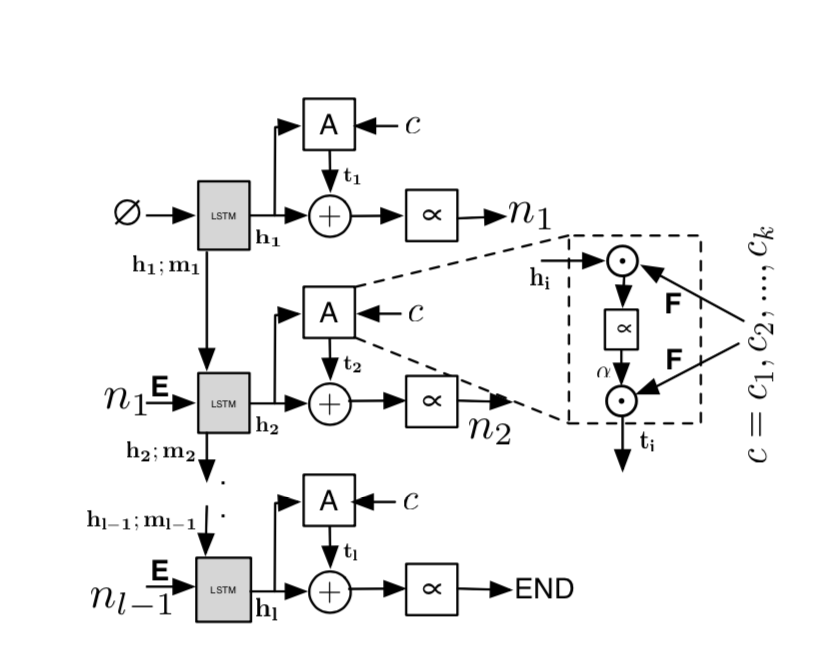
\includegraphics[width=0.5\linewidth]{ModelPics/Iyer_etal.png}
    \caption{Iyer et als Code NN, taken from \cite{iyer_summarizing_2016}}
    \label{fig:Iyer}
\end{figure}

\cite{loyola_neural_2017}




%  %drew inspiration from successes in recurrent neural networks in language modelling (CITE), and
% used of a neural attention model over source code tokens, combined with an LSTM accepting sequences of natural language tokens, to give distributions over the next token in the sequence.
% Specifically they modelled the probability of generating a length $l$
% descriptive sequence as a product of conditional probabilities the previous $l-1$ tokens
% % word sequence as a product of conditional probabilities over the next word, derived from the attentions and hidden states of the LSTM.
% % 
% $$P(\{n\}) = \prod_{i=1}^lp(n_i | n_1, ..., n_{i-1} ) $$

% where each conditional distribution was proportional to the combinations of the attentional representation and hidden state of the LSTM at that time.

% $$$$

% where 
% over the next word, whether the probabilities 

%  a distributional representation (PARA) of the source code would be calculated by an attention mechanism \cite{luong_effective_2015}, before being combined in addition with the hidden state $h_i$ of an LSTM (cite shmidthuber) and passed through a softmax layer to chose the next word in the description sequence. Each sequence 

 Summaries of Code changes - 


% Hindle's work  


% They built on work by Hindle, supported by SU
% This work ignores semantic information that could be benefitial. 

% This work specifically occurs at the level fo programming comments,

% A number of other pieces of work have since worked higher level summaries of code.
% Sridhara etc al templates
% Code NN summarization
% Related to semantic parsing - inverted. 
% Summaries of Code changes - 

% At the other end of the spectrum, code naming is treated a extremem summarization task, and has seen development.
% Other related tasks ro such include variable naming.

All
% \chapter{Theoretical Background}
\label{theoreticalbackground}




\section{Neural Network Translation Models} % (fold)
\label{sec:lstm}

\subsection{Recurrent Neural Networks for Language Modelling} % (fold)
\label{sub:recurrent_neural_networks}

\subsection{Sequence to Sequence Architectures} % (fold)
\label{sub:sequence_to_sequence_architectures}

\subsection{Attention} % (fold)
\label{sub:attention}

\subsection{Backpropagation} % (fold)
\label{sub:backpropagation}
% subsection sequence_to_sequence_architectures (end)
% subsection recurrent_neural_networks (end)

\blindtext

\section{Structure of Code} % (fold)
\label{sec:translating_code}

\subsection{Function Declarations} % (fold)
\label{sub:function_declarations}

\subsection{Abstract Syntax Trees} % (fold)
\label{sub:abstract_syntax_trees}


% subsection working_with_rnns_&_tress (end)
% subsubsection encoding_trees (end)
% subsection abstract_syntax_trees (end)

\blindtext

\chapter{Background}
\label{background}

In this section we present an overview of the theoretical items to necessary to our task of generating natural language from code features.
We start with an overview of language models, defining what they are, and noting where our task fits in the traditional NLP tasks of conditional langauge generation.
Then we provide an overview of the relevant representation learning techniques we use to achieve our goal.
Finally we conclude with a brief overview of the structure of source code, in particular its representation as an Abstract Syntax Tree. 

% In this section we first present an overview of the theoretical items necessary to our task of generating natural language from code features.
% % In particular we cast our sequence generation problem in the commonly used framework of machine translation, exploring language models, translation techniques, and neural approaches to them. 
% In particular we explore the commonly used framework of machine translation, covering language models, translation techniques, and neural approaches to them. 
% We finally present an overview of the features of code that differentiate it from natural language, and conclude with a review of relevant work in the field.

\section{Language Modelling} % (fold)
\label{sec:lstm}

\subsection{Introduction} % (fold)
\label{sub:recurrent_neural_networks}

% In order to accurately model sequences of words, we often require an  require an evaluation of the true probability of distribution sequence of words.
Although natural language has the potential to be rich and complex, more often than not it is mundane and repetetive \cite{hindle_naturalness_nodate}. 
It is such repetitiveness that makes it possible to predict in many instances. For instance, in natural English the phrase ``\textit{The music is loud, turn it ...}", is much more likely to be followed by `\textit{off}', or `\textit{down}', than the word `\textit{around}'.
This is because the actual distribution of utterances is very sparse in  the vast space of possible utterances in natural language.

In our task, we seek to generate sequences of natural language, $\{y_1, y_2,..., y_n\}$ from a set of features of code, $\mathcal{C}$.
Ideally we seek to do this through maximising a probability:

$$p(y_1, y_2,...,y_n | \mathcal{C}) \propto p(\mathcal{C} | y_1, y_2,...,y_n )  p(y_1, y_2,...,y_n )$$

where the proportionality follows from Bayes' rule.
This $p(y_1, y_2,...,y_n )$ term in this equation represents the probability of the sequence occuring naturally in the language. This term is what typical language models aim to represent.

Language models are an unsupervised means of determining the natural distribution of utterences in a language (or corpus). 
Often these utterences are broken down into single token sequences, and the probabilities are formed as a product of conditional probabilities.

$$p(y_1, y_2,...,y_n ) = p(y_n | y_1, y_2,...y_{n-1} )  p(y_1, y_2,...y_{n-1} )$$
$$= p(y_n | y_1, y_2,...y_{n-1} ) p(y_{n-1} | y_1, y_2,...y_{n-2} )...p(y_1)$$
$$ = \prod_{i=1}^{n} p(y_i | y_1^{i-1} ) $$ where $y_1^{i-1} =  \{y_1, y_2,...y_{i-1}\}$, the sequence of tokens from $1$ to $i-1$

These probabilities can be calculated in different ways, or under different assumptions. An n-gram model assumes a Markovian conditional independence structure, where the next token is conditionally independent of all others, given the previous $n$: 

$$ y_t \CI y_1^{t-n} \mid y^{t-1}_{t-n+1} $$
$$\therefore p(y_t | y_1, y_2,..., y_{t-1} )  = p(y_t | y_{t-n}, y_{t-n+1},..., y_{t-1}  ) $$

These models then estimate maximum likelihood probabilities from counts of occurences in corpora, and sometimes `smooth' these probabilities to overcome the sparsity of their training data.

Other models, such as neural language models, do not make such conditional indepence assumptions and use a neural network as a function approximator:

$$p(y_1, y_2,...,y_n ) = g(y_1, y_2,...,y_n)$$

In our work, we seek a conditional language model, which we can sample natural language given our conditioning code features $\mathcal{C}$. This conditional modelling is central to many tasks in natural language processing, which we elaborate in the next section.

\subsection{Conditional Generation of Language}

Many tasks in natural language processing require the generation of natural language conditioned on observations.
Three of the largest are machine translation, automatic summarization, and captioning.
In this section we briefly compare our task to these traditional fields, noting the similarities and differences task across each.

Firstly we consider machine translation. In this field, the objective is to generate the most likely sequence of a target language, $\{y_1, y_2,..., y_m\}$, given a sequence in an origin language  $\{x_1, x_2,..., x_n\}$. 
The translation seeks to maximise the probability:
$$ p(y_1, y_2,..., y_m| x_1, x_2,...,x_n )$$
The history and context of machine translation traditionally revolves around $\{y_i\}$ and $\{x_i\}$ being in different languages with the same semantic meaning. 
In this respect our task is not a typical translation task.
However, since our models will at times attempt to generate a sequence from another, many techniques pioneered in this field are highly transferrable to our task.

Secondly, the task of summarization aims to extract summaries or descriptions from a document.
Typically this involves extraction and/or abstraction of a document in the same modality or language.
Our task, generating descriptions about an element of a code document, naturally involves two distinct modalities - code as input, and english as output.
However, in the best case our descriptions should reflect a true and relevant summary of the argument.
Therefore, although ours is not a typical summarization task, it is sometimes framed that way in similar work\cite{iyer_summarizing_2016}.

A final task with a parallel to ours is that of captioning. 
The distinction from summarization in this case is that captioning involves generating text from differnet modalities - such as captioning a picture, or video clip.
The parallels with our code and language task are obvious here. However, it is perhaps unfair to describe documentation of code as `caption' when it aims to be a description of only the most important parts of the code, and aims to be succint.

In summary our task falls in between a number of traditional NLP tasks and consequently related tasks blur the boundaries of translation, summarization and captioning. In the next section we present an overview of the relevant theoretical components for our model, indicating their provenance from their respective fields.

\section{Representation Learning}

Given the maturity and prominence of neural networks \footnote{Quote someone}, we assume a basic familiarity with the topic, including linear and sigmoidal layers, multilayer perceptrons, the backpropagation algorithm and stochastic gradient descent. For those seeking a further background on this topic, we strongly recommend a number of books \cite{nielsenneural} \cite{Goodfellow:2016:DL:3086952} 



\subsection{Distributed Representations} % (fold)
\label{sub:embeddings}

The vocabulary of natural language is vast and nuanced. 
Some words may appear very different lexically yet have similar semantic meaning - for instance `big' and `large'.
Others may appear lexically similar, but have different meanings - `large' and `largesse'. 
In our language generation tasks we wish to generate words that have the correct semantics.
As such it would be helpful to find numerical representations of words that reflect their semantic meaning. 

One way of doing this is to distribute the semantic meaning over various components of a vector in a high dimensional space. In this space, `big' and `large' would be closer together than `large' and `largesse'. We could then use these representations in our natural language modelling as a form of transfer learning. Such an idea is not new \cite{hinton_distributed_nodate}, but recent applications of it have become widespread in statistical NLP. % REPHRASE but recent have shown trememendous benefits in training of models in recent years. CITE 

A traditional approach to finding distributioned representations includes counting cooccurences of words in a corpus, and performing matrix decomposition on the co-occurence matrix \cite{deerwester_indexing_1990}.  This is based on a core theory of distributional semantics dating back to Harris 1954 \cite{harris_distributional_1954}, that words which appear in the similar contexts have similar meanings. To quote linguist J.R Firth in 1957: ``You shall know a word by the company it keeps.'' \cite{Firth1957}
Other methods of capturing semantic meaning include counting occurences in local window around the word in question, and have also proved effective \cite{mikolov_efficient_2013}.

Glove embeddings, by Pennington et al \cite{pennington_glove_2014}, combine both local window methods and matrix factorization methods to derive their distributed represetations (word vectors).  
In our experiments we make use of pretrained GloVe pretrained embeddings to decode the words generated from our model, as similar work has demonstrated their assistance in training $<$CITE$>$.

\subsection{Recurrent Neural Networks} % (fold){}
\label{sub:recurrent_neural_networks}

Much of the semantic meaning of language is captured in the order of words. 
% It is not only the lexical tokens, but the sequence of them, that carries the information of a sentence.
This order can stretch beyond sentences, as context too can change the meaning of a sentence or phrase.
Vanilla neural networks such as multilayer perceptrons are poorly suited to capturing such long range information, as they are unable to remember preceding tokens in a sequence. 
Furthermore, they struggle from problems of vanishing and exploding gradient when processing long sequences \cite{bengio_learning_1994}.

A recurrent neural network (RNN) is one in which a hidden state is maintained by the network, while processing a sequence.
This hidden state allows information from previous tokens to propagate inside the network and contextualise the processing of future tokens.
Such networks have proved highly adaptable to language tasks, and enjoy widespread use within many sequence learning settings\cite{lipton_critical_2015}. They are also more resistant to the vanishing and exploding gradient problems.

An example of an RNN used in our research is that of the Long Short Term Memory Unit (LSTM)\cite{hochreiter_long_1997}. These comprise of four gating mechanisms, ($f_t, i_t,\tilde{c_t}, o_t$), operating on the input $\mathbf{x_t}$ and state vectors $\mathbf{c_t}$ and $\mathbf{h_t}$
\cite{noauthor_understanding_nodate}. Each gating mechanism has a corresponding weight matrix, $W$, and bias vector $\mathbf{b}$, and operate according to the following equations:

\begin{equation}
    \mathbf{f_t} = \sigma(W_f [\mathbf{h_{t-1}}, \mathbf{x_t}] + \mathbf{b_f})
    \label{eq:lstm1}
\end{equation}
\begin{equation}
    \mathbf{i_t} = \sigma(W_i [\mathbf{h_{t-1}}, \mathbf{x_t}] + \mathbf{b_i})
    \label{eq:lstm2}
\end{equation}
\begin{equation}
    \mathbf{o_t} = \sigma(W_o [\mathbf{h_{t-1}}, \mathbf{x_t}] + \mathbf{b_o})
    \label{eq:lstm3}
\end{equation}
\begin{equation}
    \mathbf{\tilde{c_t}} = \text{tanh}(W_c [\mathbf{h_{t-1}}, \mathbf{x_t}] + \mathbf{b_c})
    \label{eq:lstm4}
\end{equation}
where [,] operator indicates concatenation and $\sigma$ indicates point-wise sigmoidal function.

These gating equations then combine to update the cell state $\mathbf{c_{t-1}}$ and the hidden state $\mathbf{h_{t-1}}$ as follows: 
\begin{equation}
    \mathbf{c_t} = \mathbf{f_t} * \mathbf{c_{t-1}} + \mathbf{i_t} * \mathbf{\tilde{c_t}}
    \label{eq:lstm5}
\end{equation}
\begin{equation}
    \mathbf{h_t} = \mathbf{o_t} * \text{tanh}(\mathbf{c_t})
    \label{eq:lstm6}
\end{equation}

where  $*$ indicates point-wise multiplication, and tanh indicates point-wise hyperbolic tan.

Interpretting these operations gives a good insight into the success of the LSTM.  
Equation \ref{eq:lstm1} represents the creation of a `forget' gate, where vector $\mathbf{f_t}$ represents what fraction of each dimension of $\mathbf{c_{t-1}}$ to retain. 
Equation \ref{eq:lstm2}  creates an `input' gate, where vector $\mathbf{i_t}$ represents what fraction of each dimension of our transformed input $\mathbf{\tilde{c_{t}}}$ we want to retain.  
$\mathbf{\tilde{c_{t}}}$ itself is created in equation \ref{eq:lstm4}. With both the `input' and `forget' gate, the  the cell state is updated in \ref{eq:lstm5}. 
The new hidden state $\mathbf{h_{t}}$ then derives from this cell state, which is modified by the output gate $\mathbf{o_t}$. 
Both $\mathbf{c_{t}}$ and $\mathbf{h_{t}}$ pass forward to the next time step, while $\mathbf{h_{t}}$ is also out put by the cell. 
A diagram is presented in Figure \ref{fig:lstm_colah}

\begin{figure}[tb]
    \centering
    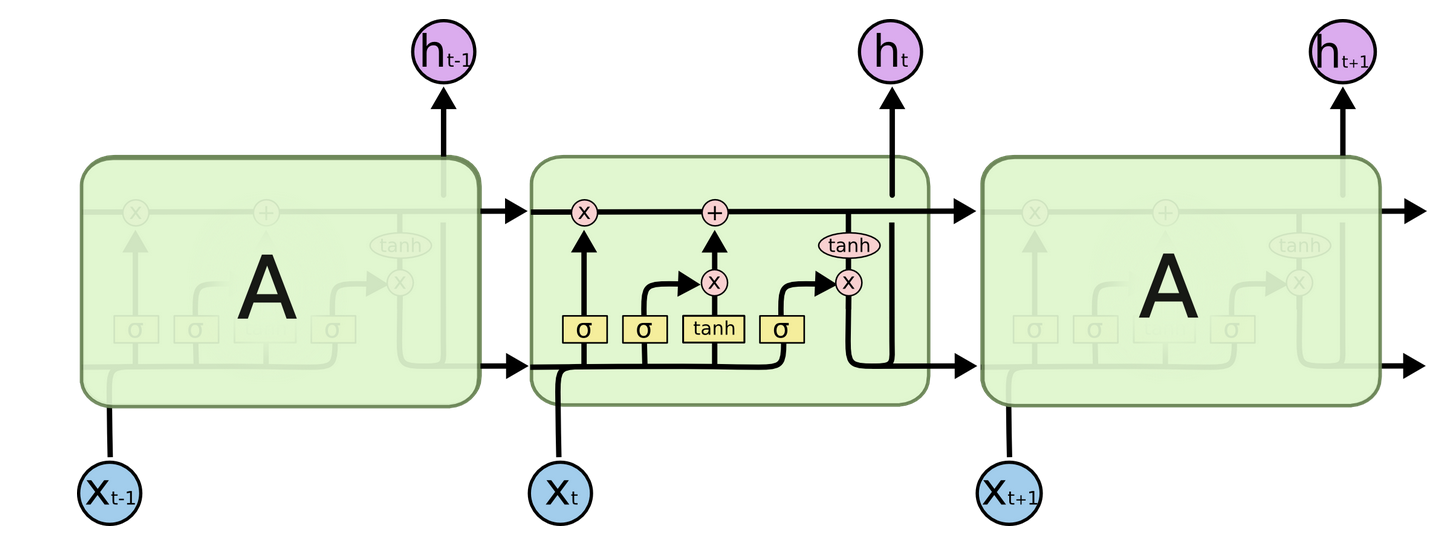
\includegraphics[width=\linewidth]{ModelPics/LSTMcolah.png}
    \caption{A diagram of an LSTM, sourced from \cite{noauthor_understanding_nodate}}
    \label{fig:lstm_colah}{}
\end{figure}

LSTM's have shown a remarkable versatility and strength in NLP tasks, not least in language modelling. A remarkable study of language modelling in 2017 showed that well-tuned LSTM architectures still surpass more recent and complex architecture, and can achieve state of the art results, despite their relative simplicity\cite{melis_state_2017}.

There also exist other forms of RNN units. The Gated Recurrent unit \cite{cho_properties_2014}, is another recurrent network unit that aims to simplify the LSTM, and has shown comparable performance to the LSTM in tasks such as speech signal modelling and music modelling \cite{chung_empirical_2014}.
However, for the purposes of our investigation, we use the LSTM for all recurrent units.

%BIDIRECTIONAL LSTMS??

\subsection{Sequence to Sequence Architectures} % (fold)
\label{sub:sequence_to_sequence_architectures}

At each time step, an RNN unit accepts an input $\mathbf{x_t}$ and emits an output $\mathbf{h_t}$. In the translation context, this 1-to-1 mapping of input to output is the equivalent of translating a sentence before you hear the end of it. For languages such as German, where the verb comes at the end of the sentence, this is almost impossible.

\begin{figure}[tb]
    \centering
    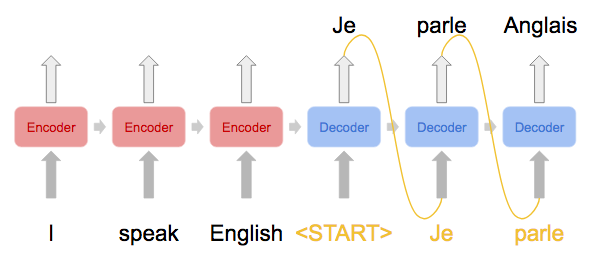
\includegraphics[width=\linewidth]{ModelPics/seq2seq.png}
    \caption{An example of sequence to sequence architecture}
    \label{fig:seqtoseq}
\end{figure}

The sequence-to-sequence architecture, originally proposed by Sutskever et al \cite{sutskever_sequence_2014}, overcomes this limitation by processing the whole input sequence before translation even begins. 
In this framework, presented in figure \ref{fig:seqtoseq}, an rnn unit such as an LSTM acts as encoder, through which all word tokens are passed. Then the final hidden states of the encoder cell are used as the initial states of a decoder rnn cell.

This decoder is then used to sequentially generate a series of tokens, by conditionally choosing the word after its input. First a ``start-of-sentence" token is fed in, generating a distribution over the vocabulary in the target language. Then most likely word is chosen, and fed back in to the decoder, generating a distribution of the next word. This method repeats until the sequence terminates, perhaps with a termination token.

In effect this results in a greedy form of decoding, where the most likely next word is continually selected from the decoder.  Other methods seek to explore the broader space of translations, by feeding in multiple tokens and retaining only the most likely sequences. This technique is known as beam search.

This architecture, though effective, has some drawbacks. It has been shown that as the source sequence gets longer, the performance of the model worsens significantly \cite{cho_properties_2014}. This is partly due to the fact that model must now compress more information into the intermediate vector passed between encoder and decoder. A common way of dealing with such an issue is to use attention, as described in the next section. 

% What are the problems: long sequences
% Forgetful of what happens at the beginning - bi rnns
% Application to machine translation. 
% Raw code tokens to language - limited success



\subsection{Attention} % (fold)

\begin{figure}[tb]{}
    \centering
    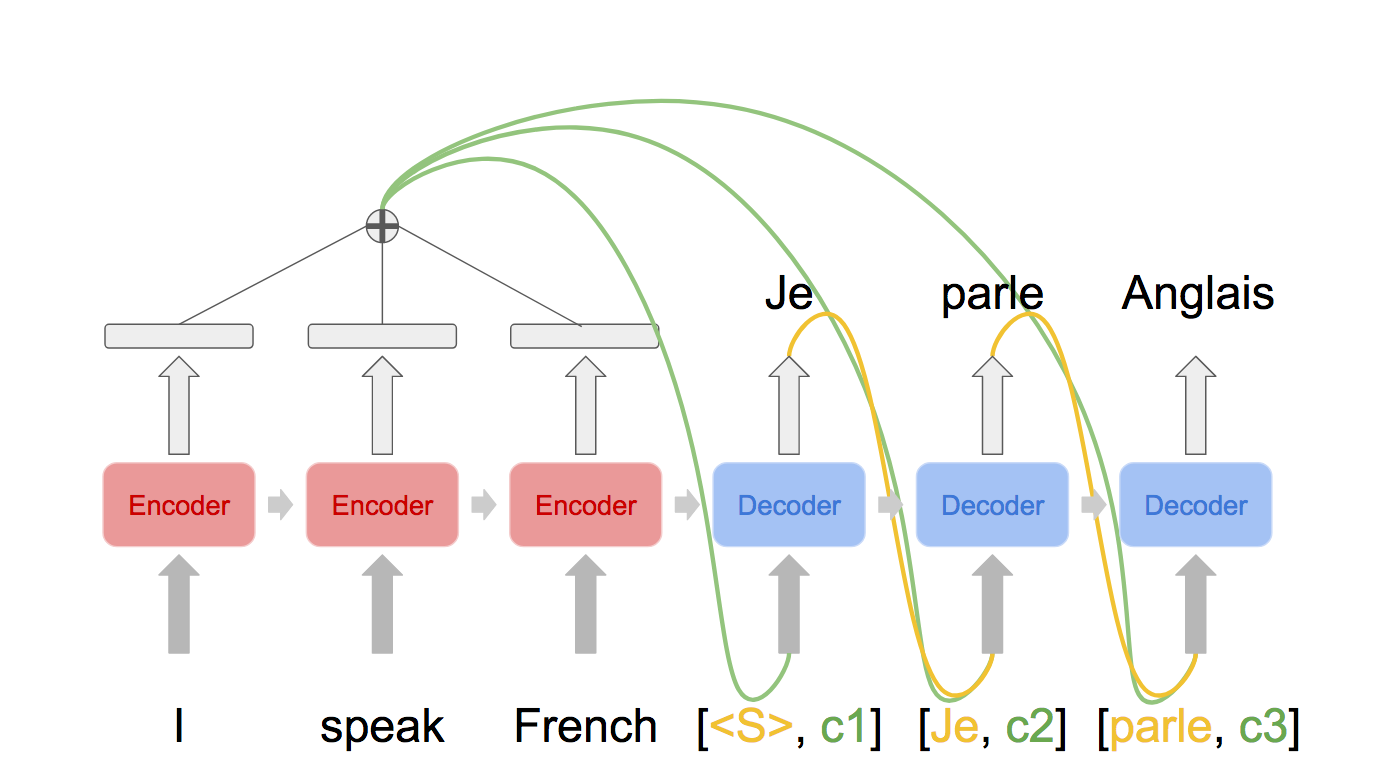
\includegraphics[width=\linewidth]{ModelPics/attention3.png}
    \caption{An example of sequence to sequence architecture with attention}
    \label{fig:attention}
\end{figure}


As the sequences get longer, encoder-decoder architectures struggle to pass the full information required from the encoder to the decoder. 
One way of improving this is to augment the decoder with a contextual vector at each step (see figure \ref{fig:attention})
As before, the decoder estimates the conditional probability for the next word $y_t$, given the input sentence $\mathbf{x}$, and previous output tokens ${y_1, ..., y_{t-1}}$.
 However, this changes from being a function of simply the input token, $y_{t-1}$, and hidden state, $s_{t}$ at step $t$:
\begin{equation}
p(y_t| y_1, ..., y_{t-1}, \mathbf{x} ) = g(y_{t-1}, s_t)
\end{equation}

to now being a function of the context vector at that point $c_t$ aswell:
\begin{equation}
p(y_t| y_1, ..., y_{t-1}, \mathbf{x} ) = g(y_{t-1}, s_t, c_t)
\end{equation}

The context vector at each step is itself calculated using a weighted sum of the rnn outputs $\{h_1,... h_{t_1}\}$:

\begin{equation}
c_t = \sum_{j=1}^{T_x}\alpha_{tj}h_j
\end{equation}
where
\begin{equation}
\alpha_{tj} = \dfrac{\text{exp}(a(s_{t-1}, h_j))}{\sum_k^{T_x}\text{exp}(a(s_{t-1}, h_k))}
\end{equation}
and $a$ is a function that maps to the reals - often a multilayer perceptron that is trained simultaneous to main training. 





This method was introduced by Bahdenau et al \cite{bahdanau_neural_2014} who demonstrated that the networks could use the attention to align words during translation.
In this case the $\alpha$ parameter acts like a weighting indicating the most important word used in each token generation - which word the decoder should pay attention to.

Variations on attention have found great use in the field of machine translation  \cite{luong_effective_2015}, and have even demononstrated their use independently of RNNs\cite{vaswani_attention_2017}. However they also have demonstrated their effectiveness in fields such as captioning, where they prove an effectve way of working with different modalities \cite{xu_show_2015}.

In our models we use attention mechanisms extensively, both as a means of dealing with particularly long sequences (in our case of characters), and also as a means of dealing with the difficult modality of code.




\section{Introduction to Python Code Structure} % (fold)
\label{sec:translating_code}


In this section we provide a brief overview of the Python programming language for readers to whom it may be unfamiliar.
We mainly annotate a typical function, provide a glossary of terms and an introduction to the Abstract Syntax Tree.

\subsection{Function Declarations} % (fold)
\label{sub:function_declarations}

Python is a dynamically typed language, meaning that the `type' of an object, such as string, integer, list or list can be decided at runtime, rather than specified in advance.
This allows a greater flexibility in the language, but comes at the expense of a less informative source code.
Declaring a variable \mintinline[]{python}{x}, makes no guarantees on what it could be, or how it can be used. 
This makes documentation an important part of Python.

In Python, functions have a built-in convention for containiing documentation - called a docstring. A typical function with a docstring is illustrated in fugure X.


\subsection{Abstract Syntax Trees} % (fold)
\label{sub:abstract_syntax_trees}

\subsection{Representations of Trees}


\section{Related Work in Source Code Modelling}

As mentioned in the Introduction, it is only through the recent development of large open source datasets that statistical approaches to code related tasks have been available to machine learning researchers. 
As would be expected of any new and growing field, the range of attempted tasks is still expanding. 
Although as of writing no formal attempt has been made to translate fine grained elements of source code into their natural language descriptions, a great deal of relevant insight has been made in the related fields of source code summarization, variable naming, documentation generation, and code language modelling. Many of these problems highlight possible approaches to modelling the patterns and structure of code as language, and can even be cast into a machine translation framework.  

In this review we summarise the current advances of these methods and how they relate to the task at hand.  We start by examining with the general progress in the language modelling of code, before moving on to specific tasks that can be posed as sequence generation tasks, such code comment prediction, code summarization or function naming. We subsequently examine advance in the related fields of representation of programs, before we finally examine the existing datasets, and the scope of the problems they are suitable to address. 

\subsection{Language Models of Source Code}

The earliest work modelling source code with natural language techniques comes from Hindle at al \cite{hindle_naturalness_nodate}, who used simple Kneser-Ney smoothed n-gram models of code tokens, to create language models for large-scale Java and C projects.
With these models, Hindle was able to demonstrate that the cross-entropy of source code within projects was lower than that of large English corpora - indicating the presence of repetetive common patterns that could be leveraged for code completion, naming and summarization.
This was consistent with findings by Gabel and Su \cite{gabel_study_2010} who examined the lines of approximately 6000 projects of code and found widespread repetition of sections of up to several lines, both within and across projects.
Despite the simplistic Markov chain assumption implicit in the ngram model, the effectiveness of this modelling techniques, especially within projects, opened up the field of code analysis to the wider natural language processing community.

This model, which only took into the lexical structure of code, was subsequently improved by Nguyen et al\cite{nguyen_statistical_2013}, who integrated semantic information into the n-gram model.
Instead of training on the raw string of the token, the \textit{lexeme}, this model condensed information such as data type, scope, role (such as literal, variable, function call) into a \textit{sememe}, and trained an n-gram topic model, modelling both local context \textit{sememes} ngrams, and global trends in the code.
This highlighted the value of taking into account the semantic information in code, as well as the lexical, in future prediction tasks.

Since then a number of different language models of code have formed, largely finding their use in code completion tasks. These are often most successful if they can take into account the long range dependencies of code, or elements of the code beyond simple lexical structure. For instance Tu et al added a cache mechanism to improve Hindle's ngram model in capturing long range dependencies  \cite{tu_localness_nodate}, while this itself was surpassed (up to 9 grams) with a basic recurrent neural language model by White et al\cite{white_toward_2015}.
Most recently, Bhoopchand et al used a sparse pointer network to create a language model that significantly outperformed a LSTM baseline on code completion tasks, that was able to refer to objects in code over 60 tokens previous\cite{bhoopchand_learning_2016}.

This work in language modelling has direct applicability to our task at hand, as it points out relevant strategies in picking out the statistically important features of `natural' code. In particular we note the importance of capturing long range dependencies (as seen in neural models), with the performance benefit that can be brought by taking into account semantic information (from the instructions given to the computer).

\subsection{Sequence Generation from Code}

Given the industrial importance of software engineers understanding sections of code, a long running task is that of code summarization. 
This task involves taking large sections of code blocks, and summarising its meaning in natural language. It has historically had parallels with the long running (inverse) problem of semantic parsing. CITE
As such, early approaches to this problem completely ignored the `naturalness' properties of code and its comments, and instead, automatic summarization of source code was tackled with rule-based methods. 

Work by Sridhara et al \cite{sridhara_[not_2010}  used static analysis to find important semantic subunits of code in Java projects, and used sets of sentence templates to produce English from these subunits.
% This model revolved around automatic rule-based summarization of the source code in the source code in consideration.
This work produced text that describe the functions in question to a high degree of accuracy, but Sridhara noted the potential lack of transferrability to other settings, and lack of examples with which to compare their summaries.  
This procedure was also inherently inflexible, relying on human crafted templates, and specified rules. Furthermore the size of the dataset, four projects in total, indicated a potential problem in the generalisability of the work to other domains, projects or even languages.

However, the advent of the statistical approaches to code language modelling led by Hindle et al \cite{hindle_naturalness_nodate} signalled the start of similar approaches to sequence generation. The earliest is Movshovitz-Attias et al \cite{movshovitz-attias_natural_nodate}, who used both ngrams and topic models such as LDA to predict comments from JAVA source code. In this they found that modelling the lexical components of source code as coming from a mixture of topics - "code" and "text" - outperformed models that ignored this distinction.  This pointed to the strength of taking into account features of code (such as distinguishing comments from commands), even if such destinction were still purely on the lexical level.

% Since then, statistical approaches have become more popular in attacking the problem, often involving much larger corpora of training data.
% Iyer et al \cite{iyer_summarizing_2016} sourced a large dataset of code snippets and questions from Stack Overflow, a popular programming website, to attempt this problem statistically.
Since then neural models have become popular methods of attacking sequence generation, as they capture long range dependencies in sequences, and have shown great promise in other neural translation tasks.

A particularly successful example is that of Iyer et al \cite{iyer_summarizing_2016}, who applied a neural attentional model to the problem of generate code summaries, training on a large collection of snippets and questions from the Stack Overflow.   Their model combined two features: a distributed representation of the code, generated by an attentional mechanism \cite{luong_effective_2015} over code token embeddings; and a Long Short Term Memory unit \cite{hochreiter_long_1997} to encode natural language tokens. Together these generated descriptions as a sequence of conditional distributions, in an encoder-decoder model. 

Specifically this model calculated the probability of generating a length $l$
descriptive sequence through a product of conditional probabilities the previous $l-1$ tokens

$$P(\{n\}_1^l) = \prod_{i=1}^lp(n_i | n_1, ..., n_{i-1} ) $$

where each conditional probability was the proportional to a non-linear transformation of the combination of hidden state of the LSTM $\mathbf{h_i}$ and the attentional vector  $\mathbf{t_i}$ at that point in the sequence: 

$$\text p(n_i | n_1, ..., n_{i-1} ) \propto \mathbf{W}\text{tanh}(\mathbf{W_1h_i} + \mathbf{W_2t_i})$$

where $\mathbf{W} \in \mathbb{R}^{|N|\text{x} H}, \mathbf{W_1}$ and $\mathbf{W_2} \in \mathbb{R}^{H \text{x} H}$  and $ H$ is embedding dimensionality of words, $ N $ the vocabulary.\cite{iyer_summarizing_2016}
A visual schematic of the model is preseted in Figure \ref{fig:Iyer}.
Iyer et al then ran a beam search over the decoder to explore the space of likely sequences, and evaluated their generations using the BLEU-4 and METEOR metrics.

This model achieved a new record in the performance of the code summarization task, and outperformed rival NLP models such as MOSES, a traditional phrase-based machine translation model \textbf{CITE \& paraphrase}, and SUM-NN, another attention based summarization model using dense layers instead of LSTMs.CITE. It also achieved a first in learning to generate original sentences from arbitrary code sections, and has proved successful in other domains.  

Loyola et al \cite{loyola_neural_2017}, for instance, adapted a similar attention model to Iyers to generate short descriptions of differnces in code.
This time intead of training on a single piece of source code and questions, data was sourced to present pairs of code changes, `diffs', with comments describing the change, `commit messages'. 
In this setting, the attentional model was able to generate faesible messages, both within projects and between projects.

Both these attention models showed the effectiveness of being able to pickout relevant portions of code at different points in sequence generation, but failed to take into account the longer term correlations of the tokens in source code. In fact by only using this kind of attentional model to process source code, both models treat the source code as little more than bag of token embeddings.

In this regard, an improvement on these attentional models is that Alamanis et al \cite{allamanis_convolutional_2016}, which uses a convolutional attention network over tokens, for the task of predicting the names of functions given their body. 
%aiming to capture long range correlations in code through spatial convolutions instead of temporal hidden state.

In this model source code is split lexically in to a padded sequence of embedded tokens, over which a one dimensional convolution of fixed width is run, to create a number of attentional feature vectors $\mathbf{\{v_k\}}$.
These feature vectors are then point-wise multiplicatied with the hidden state of an rnn, $\mathbf{h_{t-1}}$, to be effectively `selected' for their relevance to next generated token, before being normalised.

This set of feature vectors is then convolved with an attention kernel, to give a set of attention weights, each corresponding to a token embedding. 
A final attention vector $\mathbf{\alpha}$ is constructed from the convex combination of the token embeddings under the attention weights, and this vector is used to generate a distribution over the next function subtoken.
An illustration of the algorithm with pseudo code is presented in Figure X.

The authors of this model apply it to both the narrow task of generatign function names, and that of code retrieval. In it they find that taking into account the long range features of the code in the convolutional model surpasses a baseline attentional model of the machine translation model originated by Bahdenau \cite{bahdanau_neural_2014}, and found that this performance was further improved by adding a cacheing mechanism to the model.

Both these attention models show the strengths that attention can provide in combining the modalities of text and code. However, a key failing of both models remains their lack of appreciation for the syntax and semantic of the underlying code.
Although Allamanis et al's model is more aware of the structure of lexical code tokens than Iyer et als, both models continue to ignore a fundamental channel of information communication through code - that of communication from human to computer.

% Other forms of machine translation? 
% Phrase based translation, 
% neural mthods, 
% pseudo code

As of writing no published work has been applied to generating documentation of source code using the syntactical structure of source code.  However, a number of pieces of work have recently started to examine such structure in other tasks. These are the topics of the next section of review.

\subsection{Representations of Code}

As mentioned previously, most work in the field of statistical analysis of code has focused on the lexical tokens of code. 
* These can be different, same meanining, miss the underlying AST
* Recently a number of of tasks have aimed to make use of different aspects of code flow:
* Program embeddings 1, 2, 
* Graphs
* Code2Vec

\section{Existing Datasets}

The scope of the tasks available to challenge researchers is naturally limited by the set of available datasets.
In a field as young as that of sequence generation from source code, there is still a limitation in the number of datasets that have been collected, cleaned and are suitable for certain tasks.
In this section we outline the current state of the available datasets, indicating why none so far is suitable the task of translation of fine grained elements of source code.

\subsection{Language Modelling Corpora}
An early, prominent corpus of data is the GitHub Java Corpus, by Allamanis and Sutton\cite{allamanis_mining_2013}. This corpus is composed of 14,800 open source Java projects, with over 350 million lines of code (LOC), and is approximately two orders of magnitude larger than the original dataset of Hindle et al. This dataset is rich and a good example of a dataset highly suited to language modelling, but is of little use for natural language problems, given how poorly documented much open source code is.
Similar language modelling corpora exist in other languages, and run in to the same problem. Bhoopchand et al \cite{bhoopchand_learning_2016} focus on high quality code, by pulling large sections of Python code from projects with more than 100 stars from GitHub, finally collecting 40 million LOC. 
Despite the quality and scale of this corpus, the lack of structured language surrounding the code makes it unsuitable to our translation tasks, let alone anything as fine grained as we would wish.

\subsection{Stack Overflow Dataset}

A commonly used dataset for code captioning and summarization tasks is sourced from a large corpus of questions and code snippets from the programming help website Stack Overflow, as generated by Iyer et al\cite{iyer_summarizing_2016}. In it, questions such as ``how do I concatenate entire result sets in mysql? ' are paired with the snippets of C\# or SQL which are responses to the question, posted by other users online.
Although widely used, this dataset suffers from a number for undesirable features for our task. 

First of all the preparation of such a dataset demonstrates a lot of arbitrary cleaning.
Since many of the responses from the website are invalid or do not quote code, the snippets in question have been found by searching for html \mintinline[]{python}{<code>} tags in the upvoted answers. 
The authors note that these sections of code often bore no real relevance to the question at hand. Therefore the authors were forced to train a semi-supervised classifier to filter only relevant snippets to the question at hand.
This convoluted pipeline runs the risk of increasing the number anomalous datapoints in the dataset, whilst reducing almost a million (query,snippet) pairs from each language, down to 66,000 pairs  of C\# and 32,000 pairs of SQL.

Furthermore, the authors noted that often the informal code snippets often contained syntactic errors, with only 12\% of SQL snippets parsing without syntactic error. They progress with a best-effort parse, but this
 lack of code quality, naturally poses a problem for our fine grained analysis of code segments, or indeed any analysis using the syntactical properties of code.

Finally the dataset itself lacks a lot of the context and information needed for the granular analysis necessary for individual sections of code. Not only is the natural language not tailored to specific parts of the code, but the artificial snippets lack a lot of the context of real `natural' codebases. In fact, given the snippets' only relevant context is that of the question, the authors are forced to mask items like string literals and the like, to prevent the close context of the question and nothing else. This modification of the code is also undesirable.

Naturally in our search for an appropriate code base, we seek larger bigger elements of `real' (and fully parsing) code, with appropriate descriptions of elements, and a greater sense of `naturalness'.

\subsection{Edinburgh Corpus}

A recent corpus specifically tailored to code-to-text generation, is one of Python code as released by Barone and Senrich \cite{barone_parallel_2017}, which we refer to as the Edinburgh Corpus. 
This is a set of 109,000 triplets of function declarations, bodies, and documentation strings (docstrings), scraped from the most popular projects in GitHub, using the same methodology as Bhoopchand et al. 

In this dataset, the authors focus on finding real world code, and extracting the string, written by code authors, providing a description of each function.
Although these source code sections and natural language strings are more `natural', than their Stack Overflow counterparts, they still don't suit our needs, mainly in the form of the language they provide. 

Python's documentation strings are designed to be an explicit guide as to how to use the function. 
For any method in python, calling the built-in \mintinline[]{python}{help} function will display this string to the user, with the function declaration. 
Therefore this string often presents an overall view of the function, with very little reference to the inner workings of the code. 
This follows from abstraction principles of keeping library api's as a black box.
In fact from a code-readers perspective (instead of a code-users perspective), the most informative section of the docstring is where the arguments are described. 
Such a segment is not always present, but if so, would be perfect for our fine grained summarization task, as it links direct elements used in the code, to their natural-language descriptions. 

Only part of the Edinburgh corpus functions contain such such descriptions, and these are mixed in with the docstring as a whole, and therefore difficult to parse in whatever numbers they exist.
As such this makes the Edinburgh corpus limited to our needs.


\subsection{Other Datasets}
% edinburgh
% django
% stack overflow


% These attentional style models have shown great success at combining the different modalities of text and code, and this particular model
\begin{figure}[tb]
    \centering
    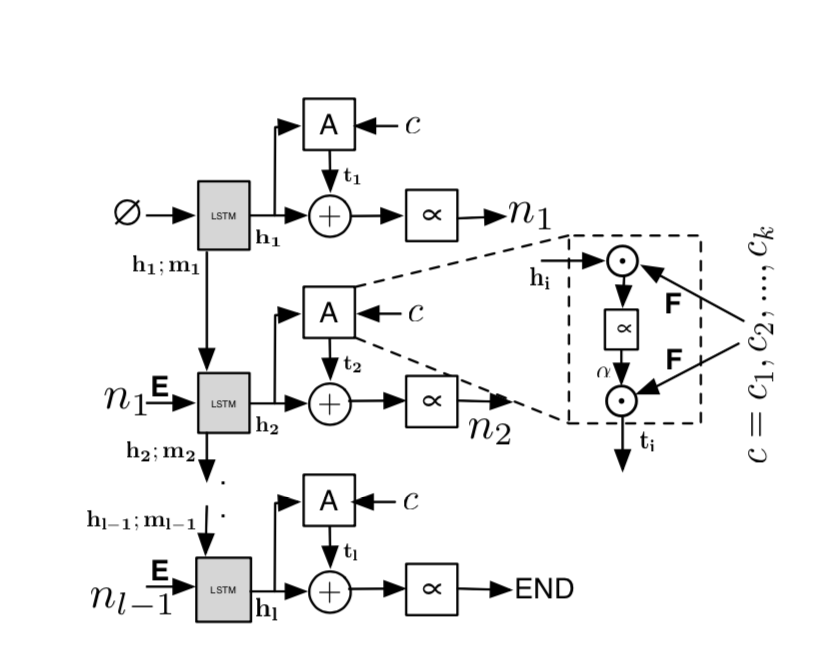
\includegraphics[width=0.5\linewidth]{ModelPics/Iyer_etal.png}
    \caption{Iyer et als Code NN, taken from \cite{iyer_summarizing_2016}}
    \label{fig:Iyer}
\end{figure}




% \chapter{Literature Review}
\section{Related Work in Source Code Modelling}

As mentioned in the Introduction, it is only through the recent development of large open source datasets that statistical approaches to code related tasks have been available to machine learning researchers. 
As would be expected of any new and growing field, the range of attempted tasks is still expanding. 
Although as of writing no formal attempt has been made to translate fine grained elements of source code into their natural language descriptions, a great deal of relevant insight has been made in the related fields of source code summarization, variable naming, documentation generation, and code language modelling. Many of these problems highlight possible approaches to modelling the patterns and structure of code as language, and can even be cast into a machine translation framework.  

In this review we summarise the current advances of these methods and how they relate to the task at hand.  We start by examining with the general progress in the language modelling of code, before moving on to specific tasks that can be posed as sequence generation tasks, such code comment prediction, code summarization or function naming. We subsequently examine advance in the related fields of representation of programs, before we finally examine the existing datasets, and the scope of the problems they are suitable to address. 

\subsection{Language Models of Source Code}

The earliest work modelling source code with natural language techniques comes from Hindle at al \cite{hindle_naturalness_nodate}, who used simple Kneser-Ney smoothed n-gram models of code tokens, to create language models for large-scale Java and C projects.
With these models, Hindle was able to demonstrate that the cross-entropy of source code within projects was lower than that of large English corpora - indicating the presence of repetetive common patterns that could be leveraged for code completion, naming and summarization.
This was consistent with findings by Gabel and Su \cite{gabel_study_2010} who examined the lines of approximately 6000 projects of code and found widespread repetition of sections of up to several lines, both within and across projects.
Despite the simplistic Markov chain assumption implicit in the ngram model, the effectiveness of this modelling techniques, especially within projects, opened up the field of code analysis to the wider natural language processing community.

This model, which only took into the lexical structure of code, was subsequently improved by Nguyen et al\cite{nguyen_statistical_2013}, who integrated semantic information into the n-gram model.
Instead of training on the raw string of the token, the \textit{lexeme}, this model condensed information such as data type, scope, role (such as literal, variable, function call) into a \textit{sememe}, and trained an n-gram topic model, modelling both local context \textit{sememes} ngrams, and global trends in the code.
This highlighted the value of taking into account the semantic information in code, as well as the lexical, in future prediction tasks.

Since then a number of different language models of code have formed, largely finding their use in code completion tasks. These are often most successful if they can take into account the long range dependencies of code, or elements of the code beyond simple lexical structure. For instance Tu et al added a cache mechanism to improve Hindle's ngram model in capturing long range dependencies  \cite{tu_localness_nodate}, while this itself was surpassed (up to 9 grams) with a basic recurrent neural language model by White et al\cite{white_toward_2015}.
Most recently, Bhoopchand et al used a sparse pointer network to create a language model that significantly outperformed a LSTM baseline on code completion tasks, that was able to refer to objects in code over 60 tokens previous\cite{bhoopchand_learning_2016}.

This work in language modelling has direct applicability to our task at hand, as it points out relevant strategies in picking out the statistically important features of `natural' code. In particular we note the importance of capturing long range dependencies (as seen in neural models), with the performance benefit that can be brought by taking into account semantic information (from the instructions given to the computer).

\subsection{Sequence Generation from Code}

Given the industrial importance of software engineers understanding sections of code, a long running task is that of code summarization. 
This task involves taking large sections of code blocks, and summarising its meaning in natural language. It has historically had parallels with the long running (inverse) problem of semantic parsing. CITE
As such, early approaches to this problem completely ignored the `naturalness' properties of code and its comments, and instead, automatic summarization of source code was tackled with rule-based methods. 

Work by Sridhara et al \cite{sridhara_[not_2010}  used static analysis to find important semantic subunits of code in Java projects, and used sets of sentence templates to produce English from these subunits.
% This model revolved around automatic rule-based summarization of the source code in the source code in consideration.
This work produced text that describe the functions in question to a high degree of accuracy, but Sridhara noted the potential lack of transferrability to other settings, and lack of examples with which to compare their summaries.  
This procedure was also inherently inflexible, relying on human crafted templates, and specified rules. Furthermore the size of the dataset, four projects in total, indicated a potential problem in the generalisability of the work to other domains, projects or even languages.

However, the advent of the statistical approaches to code language modelling led by Hindle et al \cite{hindle_naturalness_nodate} signalled the start of similar approaches to sequence generation. The earliest is Movshovitz-Attias et al \cite{movshovitz-attias_natural_nodate}, who used both ngrams and topic models such as LDA to predict comments from JAVA source code. In this they found that modelling the lexical components of source code as coming from a mixture of topics - "code" and "text" - outperformed models that ignored this distinction.  This pointed to the strength of taking into account features of code (such as distinguishing comments from commands), even if such destinction were still purely on the lexical level.

% Since then, statistical approaches have become more popular in attacking the problem, often involving much larger corpora of training data.
% Iyer et al \cite{iyer_summarizing_2016} sourced a large dataset of code snippets and questions from Stack Overflow, a popular programming website, to attempt this problem statistically.
Since then neural models have become popular methods of attacking sequence generation, as they capture long range dependencies in sequences, and have shown great promise in other neural translation tasks.

A particularly successful example is that of Iyer et al \cite{iyer_summarizing_2016}, who applied a neural attentional model to the problem of generate code summaries, training on a large collection of snippets and questions from the Stack Overflow.   Their model combined two features: a distributed representation of the code, generated by an attentional mechanism \cite{luong_effective_2015} over code token embeddings; and a Long Short Term Memory unit \cite{hochreiter_long_1997} to encode natural language tokens. Together these generated descriptions as a sequence of conditional distributions, in an encoder-decoder model. 

Specifically this model calculated the probability of generating a length $l$
descriptive sequence through a product of conditional probabilities the previous $l-1$ tokens

$$P(\{n\}_1^l) = \prod_{i=1}^lp(n_i | n_1, ..., n_{i-1} ) $$

where each conditional probability was the proportional to a non-linear transformation of the combination of hidden state of the LSTM $\mathbf{h_i}$ and the attentional vector  $\mathbf{t_i}$ at that point in the sequence: 

$$\text p(n_i | n_1, ..., n_{i-1} ) \propto \mathbf{W}\text{tanh}(\mathbf{W_1h_i} + \mathbf{W_2t_i})$$

where $\mathbf{W} \in \mathbb{R}^{|N|\text{x} H}, \mathbf{W_1}$ and $\mathbf{W_2} \in \mathbb{R}^{H \text{x} H}$  and $ H$ is embedding dimensionality of words, $ N $ the vocabulary.\cite{iyer_summarizing_2016}
A visual schematic of the model is preseted in Figure \ref{fig:Iyer}.
Iyer et al then ran a beam search over the decoder to explore the space of likely sequences, and evaluated their generations using the BLEU-4 and METEOR metrics.

This model achieved a new record in the performance of the code summarization task, and outperformed rival NLP models such as MOSES, a traditional phrase-based machine translation model \textbf{CITE \& paraphrase}, and SUM-NN, another attention based summarization model using dense layers instead of LSTMs.CITE. It also achieved a first in learning to generate original sentences from arbitrary code sections, and has proved successful in other domains.  

Loyola et al \cite{loyola_neural_2017}, for instance, adapted a similar attention model to Iyers to generate short descriptions of differnces in code.
This time intead of training on a single piece of source code and questions, data was sourced to present pairs of code changes, `diffs', with comments describing the change, `commit messages'. 
In this setting, the attentional model was able to generate faesible messages, both within projects and between projects.

Both these attention models showed the effectiveness of being able to pickout relevant portions of code at different points in sequence generation, but failed to take into account the longer term correlations of the tokens in source code. In fact by only using this kind of attentional model to process source code, both models treat the source code as little more than bag of token embeddings.

In this regard, an improvement on these attentional models is that Alamanis et al \cite{allamanis_convolutional_2016}, which uses a convolutional attention network over tokens, for the task of predicting the names of functions given their body. 
%aiming to capture long range correlations in code through spatial convolutions instead of temporal hidden state.

In this model source code is split lexically in to a padded sequence of embedded tokens, over which a one dimensional convolution of fixed width is run, to create a number of attentional feature vectors $\mathbf{\{v_k\}}$.
These feature vectors are then point-wise multiplicatied with the hidden state of an rnn, $\mathbf{h_{t-1}}$, to be effectively `selected' for their relevance to next generated token, before being normalised.

This set of feature vectors is then convolved with an attention kernel, to give a set of attention weights, each corresponding to a token embedding. 
A final attention vector $\mathbf{\alpha}$ is constructed from the convex combination of the token embeddings under the attention weights, and this vector is used to generate a distribution over the next function subtoken.
An illustration of the algorithm with pseudo code is presented in Figure X.

The authors of this model apply it to both the narrow task of generatign function names, and that of code retrieval. In it they find that taking into account the long range features of the code in the convolutional model surpasses a baseline attentional model of the machine translation model originated by Bahdenau \cite{bahdanau_neural_2014}, and found that this performance was further improved by adding a cacheing mechanism to the model.

Both these attention models show the strengths that attention can provide in combining the modalities of text and code. However, a key failing of both models remains their lack of appreciation for the syntax and semantic of the underlying code.
Although Allamanis et al's model is more aware of the structure of lexical code tokens than Iyer et als, both models continue to ignore a fundamental channel of information communication through code - that of communication from human to computer.

% Other forms of machine translation? 
% Phrase based translation, 
% neural mthods, 
% pseudo code

As of writing no published work has been applied to generating documentation of source code using the syntactical structure of source code.  However, a number of pieces of work have recently started to examine such structure in other tasks. These are the topics of the next section of review.

\subsection{Representations of Code}

As mentioned previously, most work in the field of statistical analysis of code has focused on the lexical tokens of code. 
* These can be different, same meanining, miss the underlying AST
* Recently a number of of tasks have aimed to make use of different aspects of code flow:
* Program embeddings 1, 2, 
* Graphs
* Code2Vec

\section{Existing Datasets}

The scope of the tasks available to challenge researchers is naturally limited by the set of available datasets.
In a field as young as that of sequence generation from source code, there is still a limitation in the number of datasets that have been collected, cleaned and are suitable for certain tasks.
In this section we outline the current state of the available datasets, indicating why none so far is suitable the task of translation of fine grained elements of source code.

\subsection{Language Modelling Corpora}
An early, prominent corpus of data is the GitHub Java Corpus, by Allamanis and Sutton\cite{allamanis_mining_2013}. This corpus is composed of 14,800 open source Java projects, with over 350 million lines of code (LOC), and is approximately two orders of magnitude larger than the original dataset of Hindle et al. This dataset is rich and a good example of a dataset highly suited to language modelling, but is of little use for natural language problems, given how poorly documented much open source code is.
Similar language modelling corpora exist in other languages, and run in to the same problem. Bhoopchand et al \cite{bhoopchand_learning_2016} focus on high quality code, by pulling large sections of Python code from projects with more than 100 stars from GitHub, finally collecting 40 million LOC. 
Despite the quality and scale of this corpus, the lack of structured language surrounding the code makes it unsuitable to our translation tasks, let alone anything as fine grained as we would wish.

\subsection{Stack Overflow Dataset}

A commonly used dataset for code captioning and summarization tasks is sourced from a large corpus of questions and code snippets from the programming help website Stack Overflow, as generated by Iyer et al\cite{iyer_summarizing_2016}. In it, questions such as ``how do I concatenate entire result sets in mysql? ' are paired with the snippets of C\# or SQL which are responses to the question, posted by other users online.
Although widely used, this dataset suffers from a number for undesirable features for our task. 

First of all the preparation of such a dataset demonstrates a lot of arbitrary cleaning.
Since many of the responses from the website are invalid or do not quote code, the snippets in question have been found by searching for html \mintinline[]{python}{<code>} tags in the upvoted answers. 
The authors note that these sections of code often bore no real relevance to the question at hand. Therefore the authors were forced to train a semi-supervised classifier to filter only relevant snippets to the question at hand.
This convoluted pipeline runs the risk of increasing the number anomalous datapoints in the dataset, whilst reducing almost a million (query,snippet) pairs from each language, down to 66,000 pairs  of C\# and 32,000 pairs of SQL.

Furthermore, the authors noted that often the informal code snippets often contained syntactic errors, with only 12\% of SQL snippets parsing without syntactic error. They progress with a best-effort parse, but this
 lack of code quality, naturally poses a problem for our fine grained analysis of code segments, or indeed any analysis using the syntactical properties of code.

Finally the dataset itself lacks a lot of the context and information needed for the granular analysis necessary for individual sections of code. Not only is the natural language not tailored to specific parts of the code, but the artificial snippets lack a lot of the context of real `natural' codebases. In fact, given the snippets' only relevant context is that of the question, the authors are forced to mask items like string literals and the like, to prevent the close context of the question and nothing else. This modification of the code is also undesirable.

Naturally in our search for an appropriate code base, we seek larger bigger elements of `real' (and fully parsing) code, with appropriate descriptions of elements, and a greater sense of `naturalness'.

\subsection{Edinburgh Corpus}

A recent corpus specifically tailored to code-to-text generation, is one of Python code as released by Barone and Senrich \cite{barone_parallel_2017}, which we refer to as the Edinburgh Corpus. 
This is a set of 109,000 triplets of function declarations, bodies, and documentation strings (docstrings), scraped from the most popular projects in GitHub, using the same methodology as Bhoopchand et al. 

In this dataset, the authors focus on finding real world code, and extracting the string, written by code authors, providing a description of each function.
Although these source code sections and natural language strings are more `natural', than their Stack Overflow counterparts, they still don't suit our needs, mainly in the form of the language they provide. 

Python's documentation strings are designed to be an explicit guide as to how to use the function. 
For any method in python, calling the built-in \mintinline[]{python}{help} function will display this string to the user, with the function declaration. 
Therefore this string often presents an overall view of the function, with very little reference to the inner workings of the code. 
This follows from abstraction principles of keeping library api's as a black box.
In fact from a code-readers perspective (instead of a code-users perspective), the most informative section of the docstring is where the arguments are described. 
Such a segment is not always present, but if so, would be perfect for our fine grained summarization task, as it links direct elements used in the code, to their natural-language descriptions. 

Only part of the Edinburgh corpus functions contain such such descriptions, and these are mixed in with the docstring as a whole, and therefore difficult to parse in whatever numbers they exist.
As such this makes the Edinburgh corpus limited to our needs.


\subsection{Other Datasets}
% edinburgh
% django
% stack overflow


% These attentional style models have shown great success at combining the different modalities of text and code, and this particular model
\begin{figure}[tb]
    \centering
    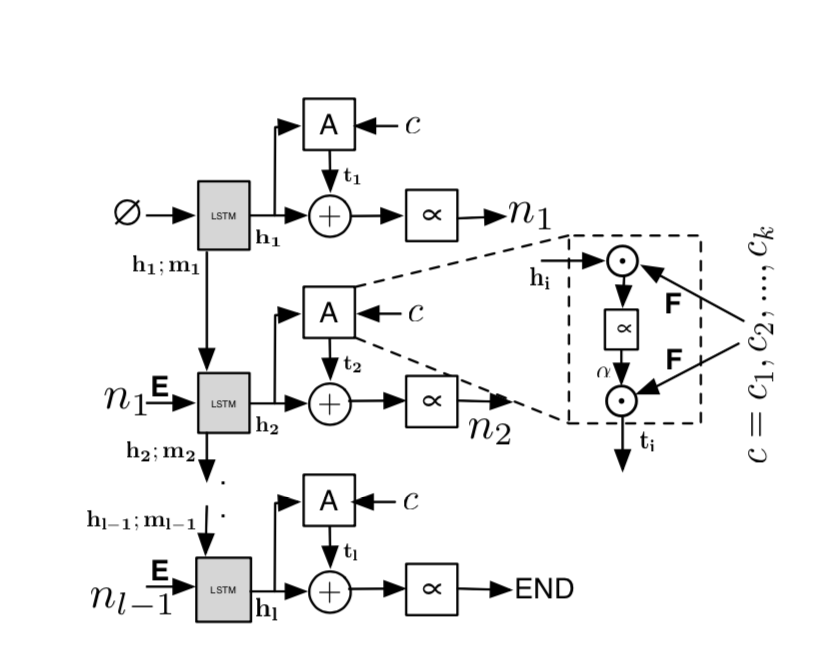
\includegraphics[width=0.5\linewidth]{ModelPics/Iyer_etal.png}
    \caption{Iyer et als Code NN, taken from \cite{iyer_summarizing_2016}}
    \label{fig:Iyer}
\end{figure}


\chapter{TheDataset}
\label{the_dataset}

\section{Method of Collection} % (fold)
\label{sec:method_of_collection}

% section method_of_collection (end)

\section{Structure of Dataset} % (fold)
\label{sec:structure_of_dataset}

% section structure_of_dataset (end)

\section{Analysis of Data} % (fold)
\label{sec:analysis_of_data}

\subsection{Statistical Analysis of Natural Language} % (fold)
\label{sub:statistical_analysis_of_natural_language}

% subsection statistical_analysis_of_natura_language (end)

\subsection{Statistical Analysis of Code} % (fold)
\label{sub:statistical_analysis_of_code}

% subsection statistical_analysis_of_code (end)

\subsection{Qualitative Analysis of Dataset} % (fold)
\label{sub:qualitative_analysis_}

% subsection qualitative_analysis_ (end)
% section analysis_of_data (end)
\chapter{Method}
\label{the_models}

% We focused on the signature because of the important nature of this section of the code. 
% In langugages such as C++, the signature of function may be all that is presented to the user of a third-party library, when using that library. 
% Therefore being able to generate reasonable descriptions from signature items alone would already be of value. 
% This does not seem an unrealistic target, since good developer practice often involves giving insightful names to variables and functions\footnote{https://github.com/google/styleguide/blob/gh-pages/pyguide.md\#s3.16-naming}.


\section{Overview}

In our investigations we focus on two main aspects of the code to generate descriptions for our arguments. 
These are the names in the function's signature, and the \textit{variable path-contexts} (VPCs) in the function's AST. 


In our experiments, we model the names of the signature as sequences of characters. We do this to capture the fact that variable and function names can often be composite and abbreviated - e.g. \mintinline[]{python}{web_ctx}. 
In this case both parts of the name might indicate a different clue to the argument:  the  \mintinline[]{python}{web} prefix may indicate a use in the internet domain; the \mintinline[]{python}{ctx} suffix may indicate a context object. 
In designing our models, we aim to pick up these patterns and conventions on the character-level.

We also focused on generating descriptions solely from the argument's VPCs. We feel that this most robust way of drawing inferences from the code, as it only examines instructions given directly to the computer. 
Any inferences here would be invariant under transformations such as renaming of variable. 
We hoped that by examining all the VPCs present for an argument, the model would learn representation for variables that indicate common usage (such as which methods are called on it), or perhaps even type.

% We chose to model this information as bag of modified `path-contexts' \cite{alon_general_2018} relevant to each variable. This would allow us to extract only the relevant sections of code pertintent to our chosen argument from the AST. 
% We hoped our models would then be able to learn which modified `path-contexts' are most informative, picking out the most relevant sections of code.

We prepared four models to investigate these data: A Rote Learner to act as baseline for our investigations; a character-level Seq2Seq Model to investigate the signature names; an original Code2Vec Decoder model to investigate the VPCs; and a Code2Vec + Seq2Seq Model to investigate both inputs combined.

The rest of this section is dedicated to presenting each of these models, summarised in Table \ref{tab:our_models_capability}, along with the  tokenization methods to obtain our data.



\begin{table}[tb]
    \centering

    \begin{tabular}{c  c  c}
          Model & Uses Signature Data & Uses VPC Data \\ 
    \hline
    Rote Learner & \checkmark & \checkmark \\
    Seq2Seq Decoder & \checkmark & \\
    Code2Vec Decoder &    &  \checkmark \\
    Code2Vec + Seq2Seq Decoder& \checkmark & \checkmark \\
    \hline
    \end{tabular}
    \caption{Overview of Our Models}
    \label{tab:our_models_capability}
\end{table}











\section{The Models}

\subsection{Rote Learner Model} % (fold)
\label{sec:rote_learner_model}

Our Rote Learner model was designed to act as a strong benchmark in all our investigations. 
It was designed according to a simple principle: \textit{the Rote Learner generates a description from a test point by returning in full a random description from a list of best-matching training point.}
It is defined formally in Algorithm \ref{alg:rote_learner_general}. 

The benefit of this model is that the definition of `best-matching' can then be changed according to the modality of the input data. In the sections below we present a brief description of these matching algorithms, with an appendix displaying each algorithm in pseudocode. A summary of these matching algorithms is presented in Table \ref{tab:matching_summary}, 

\begin{algorithm}
    \caption{The general Rote Learner algorithm }
    \label{alg:rote_learner_general}
    \begin{algorithmic}
        \Procedure{GenerateDescription}{$t$}\Comment{Generate a description for test argument $t$ }
        \State $\mathcal{M} \gets \text{BestMatchingSet}(t, training\_points)$
        \State $x \gets \text{RandomChooseOne}(\mathcal{M})$
        \State $d \gets \text{GetDescription}(x)$
        \State \textbf{return} $d$
        \EndProcedure
    \end{algorithmic}
\end{algorithm}

\begin{enumerate}
    \item \textbf{NCharacter-Gram Overlap} \textit{(Sig. Data)} \\This matching criterion was used for function signature data, and so operates on sequences of characters. It compiles a list of the training points which have the longest n character overlap with the test data point (or the longest common substring). If the same point has two of such overlaps, it is included twice, and so forth. This pseudo code is presented in Algorithm \ref{alg:ngram_overlap}.
    \item \textbf{Proportional Contexts} \textit{(VPC Data)}\\This criterion matches VPCs by treating each VPC as an atomic unit. For each VPC within the test point, the criterion finds all the training points with the same VPC. It combines these into one list, returns this list. Naturally, the list may have duplicates of the same training point. This is equivalent to choosing the training points proportionally to how often they have an overlapping VPC with the test point. The pseudocode is presented in Algorithm \ref{alg:context_algorithm} 
    \item \textbf{Max Contexts} \textit{(VPC Data)}\\This criterion takes the list output by the \textbf{Proportional Context} criterion, and only chooses the training points that appear most frequently in the list. This is equivalent to choosing the training points that have the greatest number of overlapping path-contexts with the test point. The pseudocode is also presented in Algorithm \ref{alg:context_algorithm} 
    \item \textbf{Proportional SubContexts} \textit{(VPC Data)}\\This criterion also match VPCs of the data, but treats each VPC as sequence of nodes. Specifically, as it creates $q = p{downarrow}x_f$ and treats the new path, $q$, as the sequence of nodes and arrows that compose it. This allows it to match subpaths. The matching criterion takes the test point, and for each VPC within it, finds the training VPC with the longest subsequences that matches it. It collects the corresponding datapoints to these paths and combines them into one list. It then returns this list. This is equivalent to choosing the training points that best match each VPC in the test point, proportionally to how often they are the best match. The pseudocode is presented in Algorithm \ref{alg:sub_context_algorithm} 
    \item\textbf{Max SubContexts} \textit{(VPC Data)}\\The matching criterion takes the list output by the \textbf{Proportional SubContext}, and only chooses the training points that appear most frequently in the list. This is equivalent to choosing the training points that most often are the best match for all path-contexts of the test. The pseudocode is presented in Algorithm \ref{alg:sub_context_algorithm} 
    \item\textbf{[Combinations]}\textit{(Sig. Data + VPC Data)} \\ Naturally these criteria can be combined across modalities to act upon combinations of the function signature and AST. In cases where this is done, the new list is simply the combination of the lists from the combined individual criteria. 
\end{enumerate}









\begin{table}[h!]
\makebox[\linewidth][c]{
    \centering

    \begin{tabular}{l c c p{9cm}}
    \hline
    BestMatchingSet & Use Sig. & Use AST & Description: \textit{choose list of training points...} \\
    \hline
    \hline
    NCharacter-Gram Overlap     & \checkmark & & 
         which have the longest n-character gram overlap with test \\
    % \hline
    % \hline
  
    Proportional Context  & & \checkmark & 
        which match each VPC in test, and combine\\
    Max Context  & & \checkmark &
        which match each VPC in test, combine, and take most frequent\\

    Proportional SubContext  & & \checkmark &
        which \textit{best-effort} match each VPC in test, and combine\\
    Max SubContext  & & \checkmark & 
        which \textit{best-effort} each VPC in test, combine, and take most frequent\\
    Combinations  &\checkmark  & \checkmark & 
        combine the lists from any two BestMatchingSets\\
    \hline

    \hline
    \end{tabular}
}

    \caption{An Summary of the BestMatchingSet algorithms we use in the experiments. For sake of simplicity, a \textit{best-effort} match here refers to the match with longest matching subsequence, when treating a VPC as one long sequence}
    \label{tab:matching_summary}
\end{table}





% These chose a description from a set of training samples by:
%     \begin{itemize}
%         \item combining samples with largest subpath overlap for each path in test, and chosing from that list. (Sub Path Proportional)
%         \item combining samples with largest subpath overlap for each path in test, and chosing from the most frequent training point(s) in that list. (Sub Path Max)
%         \item combining samples full overlap for each path in test, and chosing from that list (Full Path Proportional)
%         \item combining samples full overlap for each path in test, and chosing from the most frequent training point(s) in that list. (Full Path Max)
%     \end{itemize}








% subsection rote_learner_model (end)

\subsection{Character Level Sequence to Sequence Model} % (fold)
\label{sec:character_level_sequence_to_sequence}

The character level sequence model follows the standard formulation as found in \cite{bahdanau_neural_2014}

* What is the motivation of the seq to seq model.
* Since so much effort goes into naming of variables, shouldnt there be recognisable clues? Especially since,in many languages, function signature is all thats presented in documentation.
* \_ctx => context? conv2d in the function implies somethings?
* We therefore employ a sequence to sequence model to investigate the informativeness of function signatures



% subsection character_level_sequence_to_sequence (end)

\subsection{Code2Vec Decoder Model} % (fold)
\label{sec:code2vec_decoder_model}

* We then want to investigate purely without lexical names (overlap etc)
* We decide to present a modification on Code2Vec, that is argument specific.
* The motivtion is that this hsould be able to point out only some local parts of the model, the bits of the code that are near or important might get upweighted.


% subsection code2vec_to_sequence_model (end)

\subsection{Code2Vec + LSTM Encoder} % (fold)
\label{sub:code2vec_sequence_to_sequence}

Aim to combine these models together.Natural through 

% subsubsection code2vec_sequence_to_sequence (end)
% section combined_encoder_models (end)










\section{Tokenizations} % (fold)
\label{sec:tokenizations}

\subsection{Function Signature Data}

Tokenizations of the function signature data

\subsection{Abstract Syntax Trees Data }


\subsection{Argument Description}





% subsection evaluation_procedure (end)

% subsection tokenizing_code_features (end)

% subsubsection tokenizing_argument_descriptions (end)

% subsection tokenizing_textual_input (end)

% \subsubsection{Preparing the Data} % (fold)
% \label{ssub:Preparing the Data}

% \begin{enumerate}
%     \item All our data would come from one of the partitions of the dataset described in section \ref{sec:final_preparations}.

%     \item To tokenize variable names, function names and other arguments:
%     \begin{enumerate}
%         \item we generated a vocabulary of all possible tokens in valid python
%         \item We added separator tokens to the vocabulary, \mintinline{python}{"<SEPARATOR_1>"}
%         \item We then tokenizer as sequences of characters and adding an \mintinline{python}{"<END_OF_ARG>"} token to the end.
%     \end{enumerate}
    
%     \item To tokenize the argument descriptions:
%     \begin{enumerate}
%         \item We then generated a vocabulary for our training data by:
%         \begin{enumerate}
%             \item first generating a provisional vocabulary of tokens used more than 4 times in the training data.
%             \item if these words existed in our Glove embedding vocabulary they were added to our the final vocabulary. We used the  \mintinline{python}{glove.6B.200d.txt} file of 200d embeddings trained on 6 billion tokens for our Glove embeddings, (CITE). 
%             \item when this provisional list was exhausted we took the remaining most popular words, as defined by the Glove embedding file, to fill our final vocabulary to our designated "vocab-size"
%         \end{enumerate}
%         \item We then tokenized the descriptions by moving to lower case, removing new lines, and  tokenizing them using the nltk punkt tokenizer (\mintinline{python}{nltk.word_tokenize})
%         \item We then replaced out of vocabulary tokens with an \mintinline{python}{"<UNK>"} token, and finally bookending our descriptions with \mintinline{python}{"<START>"} and \mintinline{python}{"<END>"} tokens.
%         \item Path - seq?

%     \end{enumerate}



%     \item In cases of tokenized code: 
%      \begin{enumerate}
%          \item  In the case of tokenizing code paths, we first extracted the syntax tree from the source code, and traversed it exploring all paths between two nodes.
%          \item CONTINUE
%      \end{enumerate}

% \end{enumerate}

% Once these tokenizations were complete we were ready to train our models.

% \subsubsection{Training} % (fold)
% \label{ssub:training}


%     Our models were trained in the standard way:
%     \begin{enumerate}
%         \item The Rote Learner was trained determininstically, in this case using `ngram overlap' feature, as mentioned in\ref{sec:rote_learner_model}. It was evaluated with different random seeds 50 times on the hold out dataset.
%         \item The Seq-to-Seq model was trained using the backpropagation algorithm and adaptive momentum optimisation. The hyperparameters are presented in table X. 80 Epochs were evaluated, and the best and average scores were taken \textbf{EDIT}
%     \end{enumerate}




% \subsubsection{Evaluation} % (fold)
% \label{ssub:evaluation}

% % subsection training (end
% \begin{enumerate}



%     \item Finally when it came to evaluating our models on held-out datasets, we would ran translations on the dataset and calculated the BLEU score using the BLEU method found in \textbf{HERE}.
%     In particular BLEU scores were calculated over the whole corpus and \textbf{WHAT SMOOTHING HYPERPARAMTERS}.
%     \item It should be stressed that if a hyperparameter had to be tuned, it was always done on the validation set, with the test set untouched, until final evaluation. In the case of all neural models, the results presented are using the best hyperparameters under the validation set.

% \end{enumerate}









\chapter{Experiments and Results}
\label{experiments_and_results}


All experiments followed a similar general pattern of execution. 
This pattern of execution is described in detail in Section \ref{sec:experimental_setup}, which covers the general pipeline of the preparation, training and evaluation for each experiment.
Section \ref{sec:investigating_human_readable_channel} then describes the specific experiments and results of our investigations in to the human readable channel of code, whereas Section \ref{sec:investigating_the_computer_channel} covers the computer readable channel investivations.
The the results of the experiments combining these channels is presented in \ref{sec:investigating_combined_channels}, and further experiments into the dataset are presented in section \textbf{SECTION}


\section{Experimental Setup} % (fold)
\label{sec:experimental_setup}

\subsection{General Procedure} % (fold)
\label{sub:general_procedure}

% subsection general_procedure (end)

All our experiments were conducted in the same fashion, starting with a choice of dataset partition from Table \ref{table:thefinaldataset} that would be suitable to the investigation.
We would then tokenize the names and descriptions and other textual features, and if necessary extract the features we would from the code. 
These tokenization procedures and code extraction procedures are described in subsections \ref{sub:tokenizing_textual_input}, \ref{sub:tokenizing_argument_descriptions} and \ref{sub:tokenizing_code_features}.
After tokenization, the neural models would be trained on TESLA \textbf{GPUs}, for HOW long. 
These would evaluate performance on a dev set every epoch, and print translations.
How long did an epoch take.
When did we stop training.
Models were all evaluated by the same procedure as detailsed in section blah. 
%evaluated by assessing the BLEU, loss \& perplexity.


\subsection{Tokenizing Argument and Function Names} % (fold)
\label{sub:tokenizing_textual_input}

\subsection{Tokenizing Argument Descriptions} % (fold)
\label{sub:tokenizing_argument_descriptions}

\subsection{Tokenizing Code Features} % (fold)
\label{sub:tokenizing_code_features}

\subsection{Evaluation Procedure} % (fold)
\label{sub:evaluation_procedure}

% subsection evaluation_procedure (end)

% subsection tokenizing_code_features (end)

% subsubsection tokenizing_argument_descriptions (end)

% subsection tokenizing_textual_input (end)

% \subsubsection{Preparing the Data} % (fold)
% \label{ssub:Preparing the Data}

% \begin{enumerate}
%     \item All our data would come from one of the partitions of the dataset described in section \ref{sec:final_preparations}.

%     \item To tokenize variable names, function names and other arguments:
%     \begin{enumerate}
%         \item we generated a vocabulary of all possible tokens in valid python
%         \item We added separator tokens to the vocabulary, \mintinline{python}{"<SEPARATOR_1>"}
%         \item We then tokenizer as sequences of characters and adding an \mintinline{python}{"<END_OF_ARG>"} token to the end.
%     \end{enumerate}
    
%     \item To tokenize the argument descriptions:
%     \begin{enumerate}
%         \item We then generated a vocabulary for our training data by:
%         \begin{enumerate}
%             \item first generating a provisional vocabulary of tokens used more than 4 times in the training data.
%             \item if these words existed in our Glove embedding vocabulary they were added to our the final vocabulary. We used the  \mintinline{python}{glove.6B.200d.txt} file of 200d embeddings trained on 6 billion tokens for our Glove embeddings, (CITE). 
%             \item when this provisional list was exhausted we took the remaining most popular words, as defined by the Glove embedding file, to fill our final vocabulary to our designated "vocab-size"
%         \end{enumerate}
%         \item We then tokenized the descriptions by moving to lower case, removing new lines, and  tokenizing them using the nltk punkt tokenizer (\mintinline{python}{nltk.word_tokenize})
%         \item We then replaced out of vocabulary tokens with an \mintinline{python}{"<UNK>"} token, and finally bookending our descriptions with \mintinline{python}{"<START>"} and \mintinline{python}{"<END>"} tokens.
%         \item Path - seq?

%     \end{enumerate}



%     \item In cases of tokenized code: 
%      \begin{enumerate}
%          \item  In the case of tokenizing code paths, we first extracted the syntax tree from the source code, and traversed it exploring all paths between two nodes.
%          \item CONTINUE
%      \end{enumerate}

% \end{enumerate}

% Once these tokenizations were complete we were ready to train our models.

% \subsubsection{Training} % (fold)
% \label{ssub:training}


%     Our models were trained in the standard way:
%     \begin{enumerate}
%         \item The Rote Learner was trained determininstically, in this case using `ngram overlap' feature, as mentioned in\ref{sec:rote_learner_model}. It was evaluated with different random seeds 50 times on the hold out dataset.
%         \item The Seq-to-Seq model was trained using the backpropagation algorithm and adaptive momentum optimisation. The hyperparameters are presented in table X. 80 Epochs were evaluated, and the best and average scores were taken \textbf{EDIT}
%     \end{enumerate}




% \subsubsection{Evaluation} % (fold)
% \label{ssub:evaluation}

% % subsection training (end
% \begin{enumerate}



%     \item Finally when it came to evaluating our models on held-out datasets, we would ran translations on the dataset and calculated the BLEU score using the BLEU method found in \textbf{HERE}.
%     In particular BLEU scores were calculated over the whole corpus and \textbf{WHAT SMOOTHING HYPERPARAMTERS}.
%     \item It should be stressed that if a hyperparameter had to be tuned, it was always done on the validation set, with the test set untouched, until final evaluation. In the case of all neural models, the results presented are using the best hyperparameters under the validation set.

% \end{enumerate}

% section experimental_setup (end)

\section{Investigating Human Readable Channel} % (fold)
\label{sec:investigating_human_readable_channel}

% INVESTIGATION PURELY BASED ON NAME
\subsection{Comparing Baseline Models} % (fold)
\label{sub:comparing_baseline_models}

\subsubsection{Experiment Objective} % (fold)

As a baseline, we first wanted to investigate the informative power of simply the names of variables, with regards to different architectures of our baseline model.
We expected a reasonable signal to come from just the variable name which should be learnable by both our seq-to-seq model and rote learner. 

\subsubsection{Method \& Results} % (fold)

Since this experiment would only use the variable name to predict the descrption, we used the Reduced Random-Split Dataset listed in section.
This prevented inflation of BLEU scores due to exact matches being both in the train and validation set.

We then ran the standard tokenizations of input name on the Rote Learner, which only used the N-character-gram overlap criterion.
This was repeated 50 times, to provide an robust estimate of the standard deviation and mean BLEU scores, due to the inherent stocasticity to the model.

Then we ran a series of experiments on the basic Char-to-Seq architectures, starting from a basic seq-to-seq, then adding attention, a bidirectional encoder and finally dropout.
These best models were taken on the best BLEU scores up to 150 epochs, of training, and evaluated on the test and development set. % WHY 150

We report the BLEU scores in Table \ref{table:name_baseline} showing a strong performance from the Rote Learner of corpus level BLEU $9.03 \pm 0.32$ on validation and $10.60 \pm  0.30$. 
The Seq-to-Seq architectures initially underperformed the Rote Learner, scoring $7.76 $ and $  7.63$ on the validation and test set. However a marked improvement was seen by adding attention, as was adding the bidirectional encoder and dropout. 
The final model, with all addition beat the Rote Learner reasonably with a BLEU score of $12.46 $ and $12.72$ on validation and test set respectively.

The hyperparameters for these models are found in the Appendix, Table \ref{table:hyperparams_name_baseline}.
% ALL STOPPED at 150 EPOCHS. No improvement on best for 20 epochs, except original 146


\begin{table}[!ht]
\begin{center}
\begin{tabular}{ c | c | c }
    Model                             & BLEU (Validation)  & BLEU (Test)    \\
    \hline
    Rote Learner (x50)                & $ 9.03 \pm  0.32 $ & $ 10.60 \pm 0.27 $   \\
    \hline
    Seq to Seq                        & $ 8.97 $ & $ 8.18 $ \\
    + \textit{attention}              & $ 10.05 $ & $ 9.89 $  \\
    + \textit{bidirectional encoder}  & $ 11.76 $ & $ 12.34 $  \\
    + \textit{dropout}                & $ 12.68 $ & $ 12.72 $  \\
    \hline

    % Model                             & BLEU (Validation)  & BLEU (Test)    \\
    % \hline
    % Rote Learner (x50)                & $ 9.03242 \pm  0.31980 $ & $ 10.59658 \pm 0.26939 $   \\
    % \hline
    % Seq to Seq                        & $ 8.98624 $ & $ 8.17635 $ \\
    % + \textit{attention}              & $ 10.05134 $ & $ 9.88608 $  \\
    % + \textit{bidirectional encoder}  & $ 11.75615 $ & $ 12.34480 $  \\
    % + \textit{dropout}                & $ 12.67504 $ & $ 12.72236 $  \\
    % \hline
    % Seq to Seq                        & $ 4.60169 $ & $ 4.97880 $  \\
    % + \textit{attention}              & $ 4.81255 $ & $ 5.42022 $  \\
    % + \textit{bidirectional encoder}  & $ 3.00068 $ & $ 3.05952 $  \\
    % + \textit{dropout}                & $ 6.37864 $ & $ 6.33307 $  \\
    % \hline
\end{tabular}
\caption {Results of Experiment \ref{sub:comparing_baseline_models}: Comparing Baseline Models }
\label{table:name_baseline}
\end{center}
\end{table}



\subsubsection{Analysis} % (fold)

Most surprising of this result is the strength of the Rote Learner, despite there being no `exact matches' in the training and development sets. 
This is largely the result of there are arguments in the corpus with very similar descriptions, which may vary by only a few words. 

To investigate this we examined the predictions from the Rote Learner on the validation set. 
We evaluated the sentence level BLEU score on these, and found that although the vast majority evaluate to zero, a number of examples have a coincidental overlap in descriptions, resulting in a non negligible BLEU score. 
A random sample of these non-zero scored translations are presented in Figure \ref{tab:rotelearner_nameonly}.

With regard to the Seq-to-Seq, it is not surprising these standard additions to the seq-to-seq architecture improve the model. 
The addition of a bidirectional model adds capacity to the model by increasing the size of the hidden vector, and attention allows the model to condition sentence generation on the input, further adding complexity to the model.
The dropout also adds a regularizing effect.

It is perhaps surprising that the vanilla Seq-to-Seq struggles to outperform the Rote Learner. 
It is possible that the lack of contextualising information from attention results in an inability to learn from long description sequences that the Rote Learner can regurgitate immediately. 

However, once the attention and capacity are increased the results are explanatory.
The model synthesises similar (or even the same!) sequences of characters with their different descriptions, into a single description, which may fit better than randomly guessing from a bag of seen sequences. 

For instance, the most frequent argument, \mintinline[]{yaml}{name}, occurs in the train set 318 times with different descriptions. 
It also occurs 52 times in the validation set, again, with different descriptions. 
For each of these point the Rote Learner predicts a different description from the train set, on average scoring $0.00646 \pm 0.006$, whereas the Seq-to-Seq makes the same prediction each time, and scores $0.4029$, almost two orders of magnitude better, with the sensible average: ``name of the variable to return." 

In these cases the Seq-to-Seq model is interpolating in an overdetermined problem, and this highlights one of the advantages of neural networks in machine translation problems. 




\begin{table}
\begin{center}
\makebox[\linewidth][c]{
\begin{tabular}{l}
\hline\\

\textbf{A Random Sample of Bleu Scores $>0$ from Rote Learner on Random Split }\\\\ 


\textbf{Bleu Score}: 0.364
\textbf{Confidence}: 100.0\%  \\
\textbf{Argument}: \mintinline[]{python}{e d g e _ m a t c h}\\
\textbf{Description}: a function that returns true if the edge attribute dictionary for \\
the pair of nodes ( u1 , v1 ) in g1 and ( u2 , v2 ) in g2 should be considered equal during\\
the isomorphism test . if edge\_match is not specified then edge attributes are not considered .\\
\textbf{Prediction}: a function that returns true if the edge attribute dictionaries for\\
the pair of nodes ( $<$UNK$>$ , $<$UNK$>$ ) in $<$UNK$>$ and ( u2 , $<$UNK$>$ ) in $<$UNK$>$\\
should be considered equal during matching .\\

\\
\textbf{B}: 0.075
\textbf{C}: 11.1\%  \\
\textbf{A}: \mintinline[]{python}{u s e _ l o c k i n g}\\
\textbf{D}: ` bool ` . if true use locks for update operation .\\
\textbf{P}: an optional ` bool ` . defaults to ` true ` . an optional bool . defaults to\\
true . if true , the assignment will be protected by a lock ; otherwise the behavior is\\
undefined , but may exhibit less contention .\\
\\
\textbf{B}: 0.558
\textbf{C}: 12.5\%  \\
\textbf{A}: \mintinline[]{python}{y _ t r u e}\\
\textbf{D}: ground truth ( correct ) target values .\\
\textbf{P}: ground truth ( correct ) labels .\\
\\
\hline
\\
\end{tabular}
}
\end{center}
\caption{This is a random sample of sentence level BLEU scores that are non-zero fon the validation set for a Rote Learner}
\label{tab:rotelearner_nameonly}
\end{table}


% INVESTIGATION DIFFERENT TOKENIZATIONS
\subsection{Investigating Different Tokenizations} % (fold)
\label{sub:investigating_different_tokenizations}

\subsubsection{Experiment Objective} % (fold)

Having established a naive baseline and the validity of our neural approaches, we decided to investigate how other human names could help our translation problem.
We hypothesised that the names in the function signature could play an important role in contextualising an overdetermined or underdetermined variable name, further improving the performance of the LSTM relative to the Rote Learner.

\subsubsection{Method \& Results} % (fold)

We investigated how four different arrangements of input data would affect translation behaviour. 
These were:
just the argument name; the argument name with the function name; the argument name with co-argument names; and the argument name with both function name and co-argument names.

Once again we used the Reduced Random-Split Dataset, to prevent advantages due to duplicates, and ran the standard tokenization procedures outline in Sections X. 

As in section \ref{sub:comparing_baseline_models}, we ran 50 repetitions of the Rote Learner on these new tokenizations, to overcome the stochasiticity in their evaluations, once again using N-character-gram overlap as the matching criterion.

Then we ran four models of the Seq-to-Seq architectures, with attention, dropout and bidirectional encoders - just as the final model of section \ref{sub:comparing_baseline_models}. These ran for a maximum of 150 epochs, and the model with best BLEU score was selected. 

We report the results in Table \ref{table:tokenization}. 
In particular we note that in all cases the Rote Learner's performance improved with added information, in the best case, over three points to $12.22 \pm 0.23$ on validation and $14.34 \pm 0.21$ on test, thanks to the addition of the function name. 

The Seq-to-Seq model on the other hand benefitted less than the Rote Learner, if at all. In both tokenizations using other arguments, the model improved by approximately one point. However the tokenization involving the addition of just function name, saw a performance reduction of about 1.5 points, across both validation and test.

Although this agreed with out hypothesis that there is value in extra naming of variables, the under performance of the Seq-to-Seq model was surprising and is examined more fully in the analysis section.


The hyperparameters of these models are presented in Appendix Table \ref{table:hyperparams_different_tokenizations}


\begin{table}[!ht]
\begin{center}
\begin{tabular}{ c | c | c }
    Model                               & BLEU Validation            & BLEU Test  \\
    \hline
    \hline
    Rote Learner                        &                  & \\    
    - \textit{name only}                & $ 9.03  \pm  0.32 $ & $ 10.60 \pm 0.27 $  \\
    - \textit{name + function name}     & $ 12.23 \pm  0.23 $ & $ 14.34 \pm 0.22 $  \\
    - \textit{name + co-argument names}        & $ 12.06 \pm  0.16 $ & $ 14.22 \pm 0.16 $  \\
    - \textit{name + function name + co-argument names}  & $ 11.36 \pm  0.14 $ & $ 13.51 \pm 0.13 $ \\
    \hline
    \hline
    Seq to Seq                          &                  & \\
    - \textit{name only}                & $ 12.46441 $ & $ 12.72522 $  \\
    - \textit{name + function name}     & $ 10.77699 $ & $ 11.24894 $ \\
    - \textit{name + co-argument names}      & $ 13.69964 $ & $ 13.73890 $  \\
    - \textit{name + function name + co-argument names} & $ 14.13267 $ & $ 13.63351 $ \\
    % Model                               & BLEU Validation            & BLEU Test  \\
    % \hline
    % \hline
    % Rote Learner                        &                  & \\    
    % - \textit{name only}                & $ 9.03242  \pm  0.31980 $ & $ 10.59658 \pm 0.26939 $  \\
    % - \textit{name + function name}     & $ 12.22728 \pm  0.23408 $ & $ 14.33850 \pm 0.21622 $  \\
    % - \textit{name + co-argument names}        & $ 12.06262 \pm  0.16356 $ & $ 14.21676 \pm 0.16067 $  \\
    % - \textit{name + function name + co-argument names}  & $ 11.35728 \pm  0.13663 $ & $ 13.50626 \pm 0.13192 $ \\
    % \hline
    % \hline
    % Seq to Seq                          &                  & \\
    % - \textit{name only}    !!            & $ 12.46441 $ & $ 12.72522 $  \\
    % - \textit{name + function name} !!    & $ 10.77699 $ & $ 11.24894 $ \\
    % - \textit{name + co-argument names}  !!    & $ 13.69964 $ & $ 13.73890 $  \\
    % - \textit{name + function name + co-argument names}   !! & $ 14.13267 $ & $ 13.63351 $ \\
    % \hdashline
    % Seq to Seq                          &                  & \\
    % - \textit{name only}                & $ 5.54103 $ & $ 5.43827 $  \\
    % - \textit{name + function name}     & $ 4.76165 $ & $ 4.40557 $  \\
    % - \textit{name + other args}        & $ 5.70546 $ & $ 6.04723 $  \\
    % - \textit{name + function name + other args}     & $ 6.26783 $ & $ 6.24153 $ \\
    
    \hline
\end{tabular}
\caption {Investigate the effect of different code features}
\label{table:tokenization}
\end{center}
\end{table}


\subsubsection{Analysis} % (fold)
\label{ssub:analysis}

In order to probe the Seq-to-Seq model, we first investigated some of the typical setences generated by the model on the validation set.
We found that in general a number of different failings fell into either categories of overfitting or nonsense. 
Some typical examples of the model on the \textit{name + co-argument name} model are presented in Table \ref{table:typicalvarotherargs}, along with an example of a `plausible' translation. 


\begin{table}[ht!]
\begin{center}
\begin{tabular}{ l  }


\textbf{Overfitting}\\

\textbf{Input}: \mintinline[]{python}{e n c o d i n g _ t y p e <SEP-1> s e l f <SEP-2> d o c u m e}...\\
...\mintinline[]{python}{n t <SEP-2> r e t r y <SEP-2> t i m e o u t <SEP-2> <END>}\\
\textbf{Description}: the encoding type used by the api to calculate offsets .\\
\textbf{Prediction}: the encoding type used by the api to calculate sentence offsets . \\
\\\hline\\

\textbf{Nonsense}\\

\textbf{I}: \mintinline[]{python}{i n p u t <SEP-1> n a m e <SEP-2> <END>}\\
\textbf{D}: a ` tensor ` of type ` complex64 ` . a complex64 tensor .\\
\textbf{P}: ` $<$UNK$>$ ` , ` $<$UNK$>$ ` . shape is ` [ ... , m , m ] ` . \\
\\\hline\\

\textbf{Plausible}\\

\textbf{I}: \mintinline[]{python}{i n p u t <SEP-1> s t r u c t u r e <SEP-2> m a s k <SEP-2> o u t p}...\\
...\mintinline[]{python}{u t <SEP-2> b o r d e r _ v a l u e <SEP-2> o r i g i n <SEP-2> <END>}\\
\textbf{D}: binary image to be propagated inside ` mask ` .\\
\textbf{P}: binary image where a element is provided and a structuring element .\\
\\\hline\\

\\

\end{tabular}
\caption{Three examples of typical errors in the character Seq-to-Seq model.  In this case, the first example shows good use of data in the sequence but is nonsensical. The second is an example of overfitting where the predicted sentence is found in the dataset. The final case, multiple sequences such as these are found in the dataset, each with a different discription. Without looking at code, or function name (in this case) it is impossible to disambiguate and the model fails to make sense }
\label{table:typicalvarotherargs}
\end{center}
\end{table}

We then  visualized a number of attentions of the translations on the validation set, to investigate what the model was focusing on in these cases.
We found that, rather than being dispersed across multiple character tokens that might indicate useful phrases in the model, the attention focused overwhelmingly on the final tokens in the RNN in the vast majority of cases.
The attentions of the `plausible' and `nonsense' examples from  Table \ref{table:typicalvarotherargs} are visible in Figure ~\ref{fig:otherarg_attn}, demonstrating this.

\begin{figure}[ht!]
\begin{center}
    % 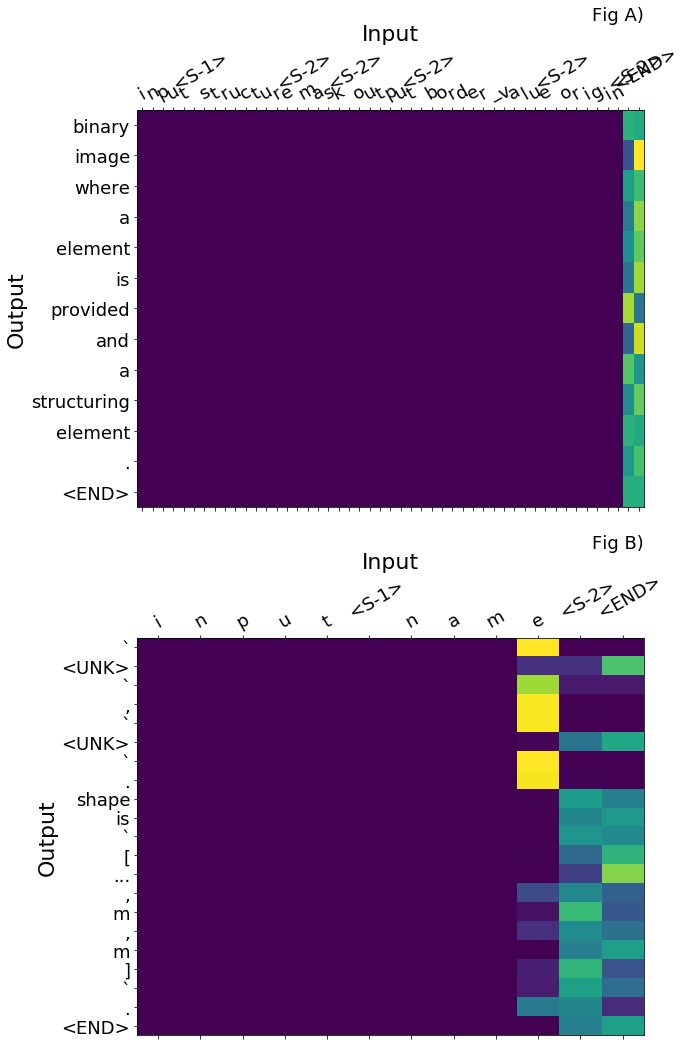
\includegraphics[width=0.7\linewidth]{images/otherargs_example.png}
    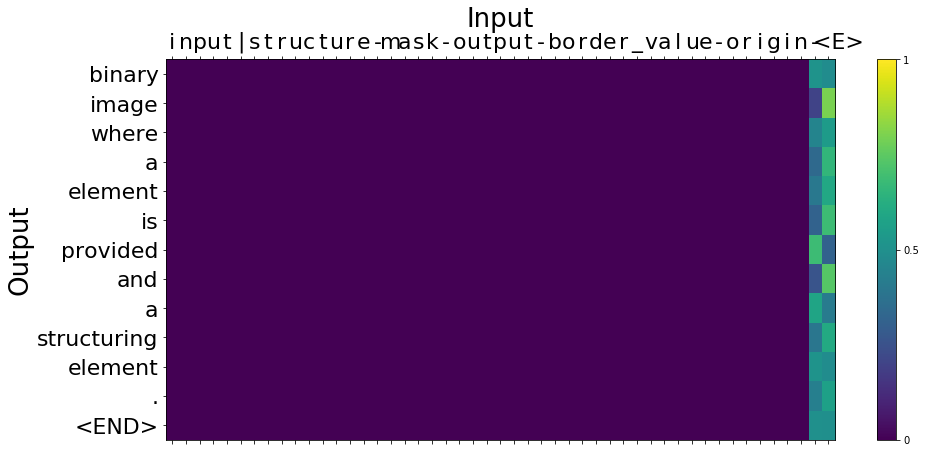
\includegraphics[width=0.9\linewidth]{ImagesCodeRelated/attn1pretty.png}
    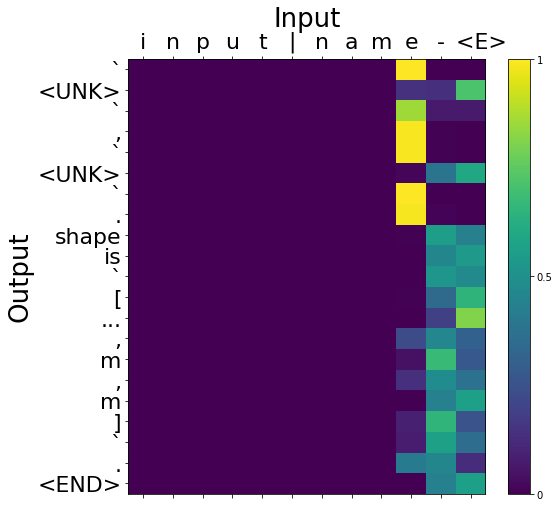
\includegraphics[width=0.5\linewidth]{ImagesCodeRelated/attn2pretty.png}
    \caption{An example of some the attentions of from the Name + Other Arguments tokenization on a Seq-to-Seq model, on the Reduced Random-Split Dataset. Fig A) is a picture of a typical example, Fig B) bottom is an example that is very overdetermined.}
    \label{fig:otherarg_attn}
\end{center}
\end{figure}

This implies the model is using all the extra information to encode a single vector to contextualise on, rather than learning to apply parts of the sequence to parts of translation, in an alignment fashion.
This single contextual vector can contain all the sequence information because the encoded RNN outputs at N can contain information from the previous N-1 tokens, and this in principle allows the model the condition word generation on the all the information up to the `attended' input token. 

Although this behaviour was expected for short sequences like variable names, we expected longer sequences (of up to 120 tokens) to be harder to compress, and suspected overcapacity of the LSTM might allow this learning strategy to take place. 
With less capacity, perhaps the final output of the RNN would not be as informative, instead relying on outputs at different points of the sequence
However, repeating the experiment with an LSTM encoder size of 75 resulted in the same pattern of attention, though with a much reduced BLEU score.

We also repeated the experiment on the much larger Full Random-Split dataset, where now just the input argument name would be certainly be the most important feature, due to repetitions points with the same name with the same description, but different co-arguments and function names. 
In this case we saw the final heavy attention shift to the separator just after the variable name - indicating that the model was learning where the most informative section of the data was, but was still choosing the encoded vector at that point. 
Interestingly we found that model did still take into account the rest of the sequence after this point (generating different translations), but that these all varied along a the same theme of the variable name. 
The attentions for a single example are given in Figure ~\ref{fig:otherarg_attn_full_dataset}

\begin{figure}

\begin{center}
    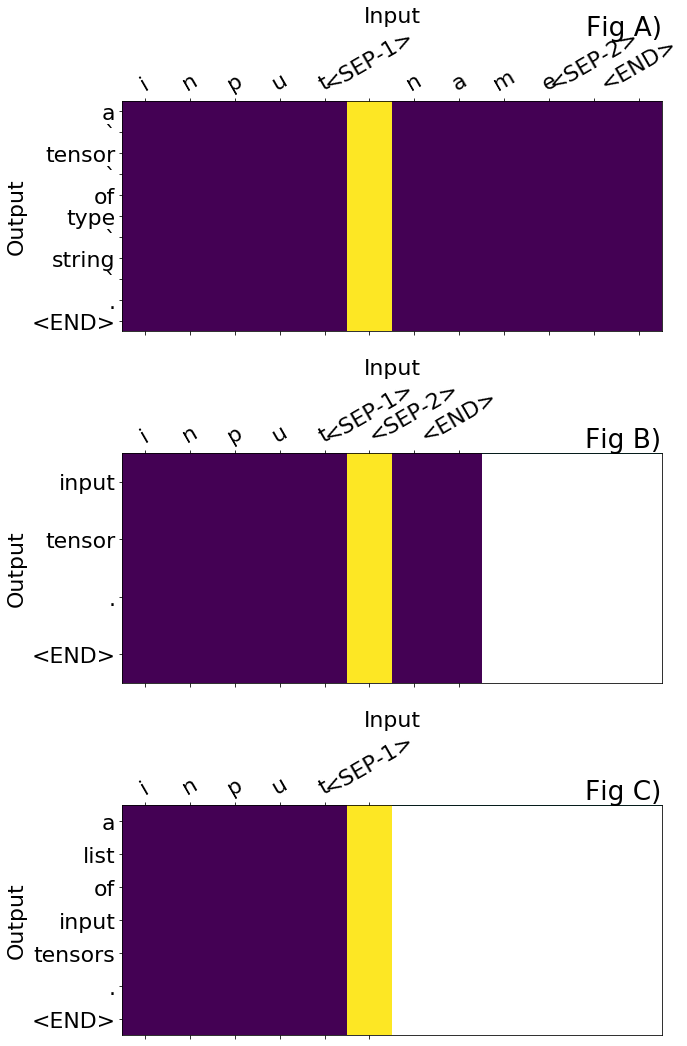
\includegraphics[width=0.7\linewidth]{images/different_translations_dupsXotherargs_3230minib_white.png}
    \caption{Three translations and attentions for an example of some the attentions of from the Name + Other Arguments on the tokenization on a Seq-to-Seq model trained on the Full Random-Split Dataset. Here is shows that, on the Full Random-Split Dataset, the most important feature is variable name, and the model attends solely to that, but that the hidden state of the LSTM still takes into account characters after the variable input }
    \label{fig:otherarg_attn_full_dataset}
\end{center}
\end{figure}

The conclusion to be drawn from this investigation is that the attention does not distribute well over characters, and these tokenizations actually behave much like longer single names, rather than features that can be distiguished separately. 
This leads to overfitting in many cases, as the some names are closer to unique, and you get a model that fits more like a Rote Learner. 
The model seems to work at its best when synthesising information as much as possible, but this seems more difficult to do when so much identifying information is given without information on redundancy. 
To give an example, Table \ref{table:example_plausible_training} shows the `plausible' example given above, with all training instances that start \mintinline[]{yaml}{input<SEP-1>structure}, highlighting that certain features of the final description are in the training ("binary image"), yet the potentially helpful sequence \mintinline[]{yaml}{<SEP-1>mask<SEP-1>} is ignored.

To counter this beahaviour in future, more work could be done both by investigating tokenizations or attention mechanisms.
In particular, the peaky nature of the softmax in attention could be replaced with a broader distribution, or the entropy of the softmax could be changed with a temperature parameter throughout training, to force the model to consider different sections of the data.
Ideally, combined with this differnet annention arrangement, more data would be provided that could help present a nuance to the arguments, rather than them simply being specifying information. 
Future work should at least investigate whether data augmentation by providing duplicates with arguments in different orders, perhaps also with synonyms of descriptions, could help models learn more generalisable descriptions.


\begin{table}
\begin{center}
\makebox[\linewidth][c]{
\begin{tabular}{l}

\hline
\textbf{Validation Example}\\

\textbf{I}: \mintinline[]{python}{i n p u t <SEP-1> s t r u c t u r e <SEP-2> m a s k <SEP-2> o u t p}...\\
...\mintinline[]{python}{u t <SEP-2> b o r d e r _ v a l u e <SEP-2> o r i g i n <SEP-2> <END>}\\
\textbf{D}: binary image to be propagated inside ` mask ` .\\
\textbf{P}: binary image where a element is provided and a structuring element . $<$END$>$\\
\\\hline\\

\textbf{Training Examples} starting \mintinline[]{yaml}{i n p u t <SEP-1> s t r u c t u r e}\\
\textbf{I}: \mintinline[]{yaml}{i n p u t <SEP-1> s t r u c t u r e 1 <SEP-2> s t r u c t u r}...\\
...\mintinline[]{yaml}{e 2 <SEP-2> o u t p u t <SEP-2> o r i g i n 1 <SEP-2> o r i g i n 2 <SEP-2> <END>}\\
\textbf{D}: binary image where a pattern is to be detected .\\
\\
\textbf{I}: \mintinline[]{yaml}{i n p u t <SEP-1> s t r u c t u r e <SEP-2> i t e r a t i o n s <SEP-2> o u t }...\\
...\mintinline[]{yaml}{p u t <SEP-2> o r i g i n <SEP-2> m a s k <SEP-2> b o r d e r _ v a l u e }\\
...\mintinline[]{yaml}{<SEP-2> b r u t e _ f o r c e <SEP-2> <END>}\\
\textbf{D}: binary array\_like to be closed . non-zero ( true ) elements form the subset to be closed .\\
\\
\textbf{I}: \mintinline[]{yaml}{i n p u t <SEP-1> s t r u c t u r e <SEP-2> o u t p u t <SEP-2> o r}...\\
...\mintinline[]{yaml}{i g i n <SEP-2> <END>}\\
\textbf{D}: n-dimensional binary array with holes to be filled\\
\\
\textbf{I}: \mintinline[]{yaml}{i n p u t <SEP-1> s t r u c t u r e <SEP-2> o u t p u t <SEP-2> <END>}\\
\textbf{D}: an array-like object to be labeled . any non-zero values in ` input ` are counted as features...\\
...and zero values are considered the background .\\
\\
\textbf{I}: \mintinline[]{yaml}{i n p u t <SEP-1> s t r u c t u r e <SEP-2> i t e r a t i o n s <SEP-2> m a s k }...\\
...\mintinline[]{yaml}{<SEP-2> o u t p u t <SEP-2> b o r d e r _ v a l u e <SEP-2> o r i g i n <SEP-2>}\\
...\mintinline[]{yaml}{b r u t e _ f o r c e <SEP-2> <END>}\\
\textbf{D}: binary image to be eroded . non-zero ( true ) elements form the subset to be eroded .\\
\\
\textbf{I}: \mintinline[]{yaml}{i n p u t <SEP-1> s t r u c t u r e <SEP-2> i t e r a t i o n s <SEP-2> m a s k}...\\
...\mintinline[]{yaml}{<SEP-2> o u t p u t <SEP-2> b o r d e r _ v a l u e <SEP-2> o r i g i n <SEP-2>}\\
...\mintinline[]{yaml}{b r u t e _ f o r c e <SEP-2> <END>}\\
\textbf{D}: binary array\_like to be dilated . non-zero ( true ) elements form the subset to be dilated .\\
\\



\end{tabular}
}
\caption{A validation example and the a selection of training points. Despite being a long sequence, }
\label{table:example_plausible_training}
\end{center}
\end{table}

%%% EXTRA PLOTS: Avergae attention over words
%%%.             Attention/Results of words shuffled



% What is the problem? Attention softmax is narrow and doesnt distribute well over characters, since there isn't really a one to one alignment. Instead what we see is the same behaviour as a much longer function name, where it works best when interpolating data. then give the plausibility

% Future work: Attention softmax is too narrow. Try a higher entropy distribution for character model
% Try a learning schedule
% Rotate the order of words, (done)
% Also more data.


% \begin{enumerate}
%     % \item we expected words to help choose bits in overdetermined cases. attention distributed across multiple words
%     % \item however we get attention focused on last word.
%     % \item The rnn final state acts as a good contextual vector for generation, we get good performance improvements on decoding
%     % \item The sort bonus is explained, but no change with longer.
%     \item It is possible the attention is being pathological. It's such a good strategy, that it stays there, and stops looking elsewhere, the weight decays to zero
%     % \item To investigate we ran with low lstm, -> no change in behaviour (LSTM 75), still tries to encode
%     \item We then tried to investigate if the rest of the data is being used (use the full dataset, and found that)
%     \item in cases with still degeneracy, attention is confused it panics (see bluring at end - can only explore nearest by states)
%     \item Check out Rote learner vs LSTM for "name" again. is it interpolating, or being a bad lstm (fitting bits of it, that dont transfer.)
%     \item We also take a closer look at the failures and notice a specific pattern. note tha in some cases the model works well, and. Basically hypothesise the size of the data with lack of indentifyin ginformation leads to overfitting, rather than just variable name which works.
% \end{enumerate}


\section{Investigating the Computer Readable Channel} % (fold)
\label{sec:investigating_the_computer_channel}

\subsection{Comparing Code2Vec to Baselines} % (fold)
\label{sub:comparing_code2vec_to_baselines}


\subsubsection{Experiment Objective} % (fold)

In our first examination of the computer readable channel we aimbed to validate our initial hypothesis that simply the code could be informative when predicting argument descriptions.
In particular we wished to assess what possible tokenizations of code paths from the syntax tree could prove most informative, and set up as strong baseline as possible against which would compare our neural model.



\subsubsection{Method \& Results} % (fold)

For this experiment we used the Full Random-Split Dataset, to make the most of the different code paths associated with each argument.
We followed the vocabulary generation and source code tokenization procedures outlined in section X. 
We used a vocabulary size of 15000 for both path strings and terminal nodes, and set the maximum number of paths per argument to  5000.
These values were sought to be as large as possible for the size of the GPU. 

We then ran our Rote Learner, using the four different matching code path only criteria, outlined in section X. 
These chose a description from a set of training samples by:
    \begin{itemize}
        \item combining samples with largest subpath overlap for each path in test, and chosing from that list. (Sub Path Proportional)
        \item combining samples with largest subpath overlap for each path in test, and chosing from the most frequent training point(s) in that list. (Sub Path Max)
        \item combining samples full overlap for each path in test, and chosing from that list (Full Path Proportional)
        \item combining samples full overlap for each path in test, and chosing from the most frequent training point(s) in that list. (Full Path Max)
    \end{itemize}
Each of these was run 50 timesto overcome the stochasticity of the Rote Learner.

We then ran the Code2Vec Decoder, following the usual training procedure, for a maximum of 100 epochs.
We selected the model with the best BLEU score in that time.
The hyperparameters for this model are found in Table {X}.

We report our results in Table \ref{table:name_code2vec_solo}, noting that the Rote Learner performed best using the Full Path Max matching, with a BLEU score $ 11.82 \pm  0.16 $ and  $ 12.61 \pm 0.12 $ on validation and test, but that the Code2Vec Decoder significantly outperformed this, achieving a BLEU score of $ 18.94 $ and $ 18.13 $ on validation and test respectively.

From the Rote Learning perspective, the next best criterion was the Sub Path Max, which achieved a corpus level BLEU score of $ 6.93 \pm  0.34 $ and $ 7.09 \pm 0.22 $ on validation and test respectively.  
The two remaining Proportional criteria performed worst, each about 6 bleu points worse than their counterparts

These results confirmed that looking at code paths would indeed be informative, and indicated that investigating full codepaths would indeed be the best way to start. 
They also showed great promise for the Code2Vec Decoder as a model.

% subsection comparing_code2vec_to_baselines (end)

\begin{table}[ht!]
\begin{center}
\begin{tabular}{ c | c | c  }
    Model                             & BLEU Validation  & BLEU Test      \\
    \hline
    Rote Learner (codeonly)                  &  &  \\
    - \textit{Subpath Proportional}              & $ 0.71 \pm  0.13 $ & $ 0.74 \pm 0.07 $   \\
    - \textit{Subpath Max}                       & $ 6.93 \pm  0.34 $ & $ 7.09 \pm 0.22 $  \\
    - \textit{Full Path Proportional}            & $ 4.94 \pm  0.28 $ & $ 5.11 \pm 0.18 $  \\
    - \textit{Full Path Max}                     & $ 11.82 \pm  0.16 $ & $ 12.61 \pm 0.12 $  \\
    \hline
    Code2Vec Decoder                             & $ 18.94 $ & $ 18.13 $  \\
    % \hdashline
    % Code2Vec                          & $ 12.64199 $ & $ 12.80257 $  \\
    \hline 
    % Model                             & BLEU Validaion  & BLEU (Test)      \\
    % \hline
    % Rote Learner (codeonly)           &  & & \\
    % - \textit{softest}                     & $ 0.70702 \pm  0.13979 $ & $ 0.73623 \pm 0.07094 $   \\
    % - \textit{soft}                        & $ 6.93465 \pm  0.33987 $ & $ 7.09349 \pm 0.21836 $  \\
    % - \textit{hard}                        & $ 4.94109 \pm  0.28153 $ & $ 5.11432 \pm 0.18345 $  \\
    % - \textit{hardest}                     & $ 11.82453 \pm  0.15695 $ & $ 12.61319 \pm 0.12093 $  \\
    % \hline
    % Code2Vec   !!                            & $ 18.93630 $ & $ 18.12909 $  \\
    % % \hdashline
    % % Code2Vec                          & $ 12.64199 $ & $ 12.80257 $ & \\
    % \hline
\end{tabular}
\caption {BLEU Scores on the Full Random-Split Dataset, for Code2Vec Decoder and a series of code only Rote Learners}
\label{table:name_code2vec_solo}
\end{center}
\end{table}

\subsubsection{Analysis} % (fold)
\label{ssub:analysis}

In order to investigate the behaviour of the Code2Vec model, we sampled points from the validation set, printed out the source code, paths and attentions as they passed through the model.
We observed that sometimes the model overfit some particular paths, with very high attentions on a single point, but more often than not the model distributed its attention over 4 or 5 paths, even if there were thousands to choose from.

A single example of such an analysis, where multiple paths are attended and the different paths are easy to see, is presented in Figure  \ref{fig:single_examples} .
It shows the pretokenized syntax tree, the attented paths, the source and the translation.
From this example it is interesting to note that the model has chosen two paths that indicate list comprehensions feature in the variable, and it has inferred that a list should feature in the description from the code alone.

Noting that the model seemed to be performing as expected on a microscopic level, we continued to investigate the behaviour of the model across the entire validation set. 
Figure \ref{fig:entropy_code2vec} shows a the distribution of the entropies of the attentions of the Code2Vec vectors, for each point in the validation set. 
Presented along side, is the distribution of entropies that would have occured if every data point in the validation set had attained a uniform, categorical distribution as attention.
The shift to a lower entropy clearly verifies that the Code2Vecs attention focuses on only a fraction of the paths, and, in some few cases (where the entropy is effectively 0) decides resolutely on single points.

Figure \ref{fig:sentence_bleu} shows the counts of sentence level BLEU score of each sentence in the validation set.
Although this metric is prone to low scores on individual sentences <CITE> over the whole corpus, we can use it to get a sense for where the performance improvements come from in the Code2Vec Model.
From this graph it is one can see both a significant increase in the models 1.0 scoring sentences, and also a modest increase in low scoring sentences. 
This indicates both an improvement that may be down to some form of overfitting (the model is able to find arguments that are very similar, and have similar code paths), but also an improvement due to generating just a few of the correct words, as in the example presented above. 


\begin{table}[ht!]
\begin{center}

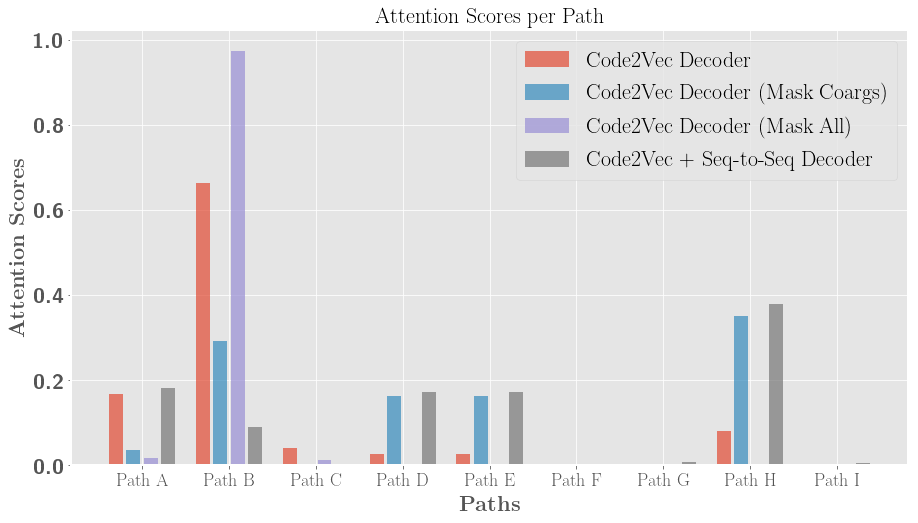
\includegraphics[width=0.9\linewidth]{ImagesCodeRelated/pretty_attention_XKCD.png}
        % how to set font size here to 10 px ?  
\begingroup
    \fontsize{10pt}{12pt}\selectfont
\begin{tabular}{c l}
    & \textbf{Paths} \\
    \\
    \textbf{Path A} & Name $\leftarrow$ comprehension $\leftarrow$ ListComp $\leftarrow$ Assign $\rightarrow$ Name : \mintinline[]{yaml}{palette} \\
    \textbf{Path B} & Name $\leftarrow$ comprehension $\leftarrow$ ListComp $\rightarrow$ comprehension : \mintinline[]{yaml}{<UNK>} \\
    \textbf{Path C} & $<$UNK$>$ : \mintinline[]{yaml}{color_palette} \\
    \textbf{Path D} & Name $\leftarrow$ comprehension $\rightarrow$ Name : \mintinline[]{yaml}{name} \\
    \textbf{Path E} & $<$UNK$>$ : \mintinline[]{yaml}{palette} \\
    \textbf{Path F} & $<$UNK$>$ : \mintinline[]{yaml}{palette} \\
    \textbf{Path G} & $<$UNK$>$ : \mintinline[]{yaml}{len} \\
    \textbf{Path H} & $<$UNK$>$ : \mintinline[]{yaml}{name} \\
    \textbf{Path I} & $<$UNK$>$ : \mintinline[]{yaml}{<UNK>} \\
\end{tabular}
\endgroup

% \caption{Example Attention Scores}
% \end{table}

\end{center}
\caption{Code \& List}
\label{fig:single_examples}
\end{table}


\begin{figure}
\begin{center}
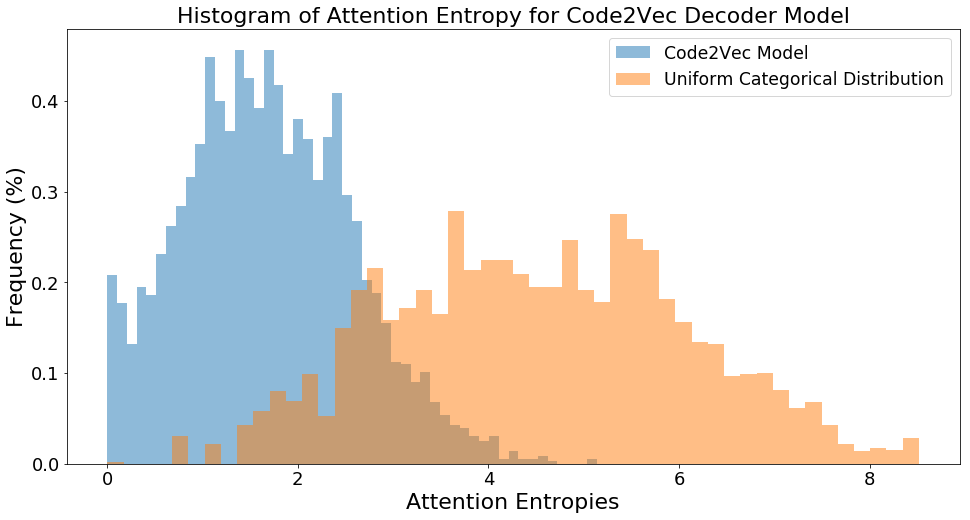
\includegraphics[width=0.8\linewidth]{ImagesCodeRelated/code2vec_entropies.png}
\end{center}
\caption{code2vec entropy}
\label{fig:entropy_code2vec}
\end{figure}


% \begin{enumerate}
%     \item With the code lstm we see some of the behaviour we like, but also, only overfitting. There is no sequence so in some cases, a path or a single variable can be informative, but it performs well.
%     \item See a single example and distribution of attention.
%     \item CLearly there are a lot of spikes compared to uniform. More masking the more spiking, though this is partly due to best bleu. Compare at cross entropy time?
%     \item Then look at, bleu per sentence, maybe av bleu per sentence per attn entropy.
%     \item Big COMPARE vs ROTE LEARNER - can we conclude this is worth more researcg?
%     \item Cna show how choices change w model for given example??

%     \item C2VEnc: does combining add anythin? More capacity, check weights.
% \end{enumerate}

% \begin{table}


% subsubsection analysis (end)

\subsection{Masking Identifiers in Code2Vec} % (fold)
\label{sub:comparing_code2vec_altered}

\subsubsection{Experiment Objective} % (fold)

The Code2Vec Decoder model uses a vocabulary of terminal nodes to generate code paths. 
Due to the python abstract syntax tree, these are almost always names, which could be either those of internal variables, built-in functions or even out of scope objects. 
We investigated masking these terminal node names, to be conclude that that the structure of the code was providing a valuable signal to the Code2Vec Decoder, beyond the ideosyncracies of variable and method naming.

\subsubsection{Method \& Results} % (fold)

We used the same dataset and tokenization procedure as described in Section \ref{sub:comparing_code2vec_to_baselines} to prepare the tokenized code paths as before.
However, this time we investigated two different masking procedures, to hide the terminal node from the models.

In the first masking, we masked the only the coarguments in the code paths.
We did this by creating new terminal node identifiers, for "first coargument", "second coargument", and so forth, and renaming all terminal node identifier indices to these numbers.
This means that the model can still recognise when two code paths belong to the same terminal node, but no embedding can be generated linking the fact that that argument shares a coargument name with any other variables.

In our second masking, we masking we repeated this procedure, but for every point in the dataset.
This meant that very indicative global variables were masked, but also any inbuilt method.
Instead the model only had access to enough information to be able to differentiate terminal nodes within a function.

Once again we trained these for 100 epochs, with the hyperparameters specified in Appendix X.

We present the results in Table \ref{table:code_2_vec_masked}, noting that Coargument Masking only resulted in a slight performance drop, of one to two BLEU points, from the unmasked variables, while the Full Masking resulted in a significant drop of six BLEU points, while still beating the best Rote Learner baseline.



\begin{table}[ht!]
\begin{center}
\begin{tabular}{ c | c | c }
    Model                             & BLEU (Unsplit)  & BLEU (Split)    \\
    \hline
    Rote Learner (best performer)          & $ 11.82453 \pm  0.15695 $ & $ 12.61319 \pm 0.12093 $ \\
    \hline
    Code2Vec                               & $ 18.93630 $ & $ 18.12909 $ \\
    Code2Vec  (Coargument Masking)              & $ 17.01868 $ & $ 16.93701 $ \\                  
    Code2Vec  (Full Masking)                & $ 13.27677 $ & $ 13.07374 $ \\
    % \hdashline

    % Code2Vec                              & $ 12.64199 $ & $ 12.80257 $ & \\
    % Code2Vec (masked args)                & $ 12.10462 $ & $ 11.93314 $ & \\
    % Code2Vec (masked all)                 & $ 9.01463 $ & $ 9.15697 $ & \\
    \hline
\end{tabular}
\caption {Investigate code2vec but with masked variables}
\label{table:code_2_vec_masked}
\end{center}
\end{table}


\begin{figure}
\begin{center}
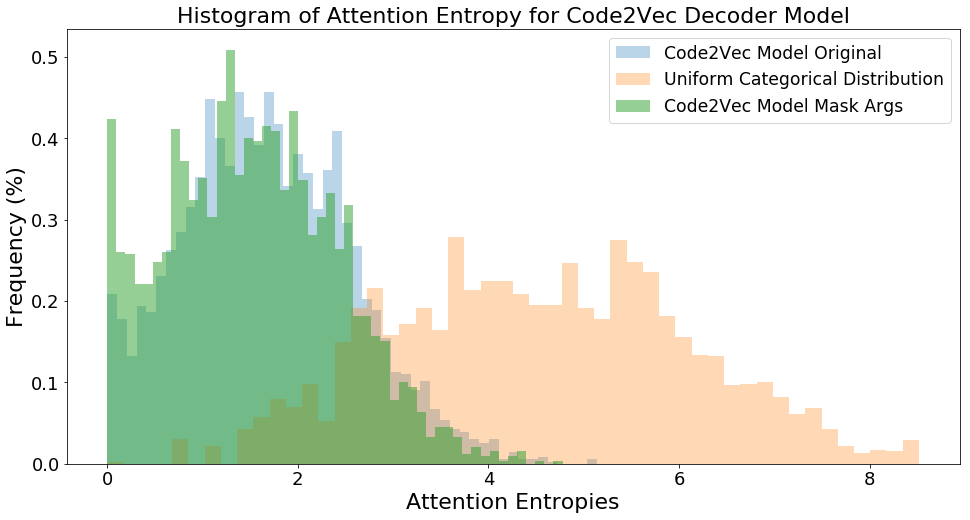
\includegraphics[width=0.8\linewidth]{ImagesCodeRelated/entropies_mask_args.png} 
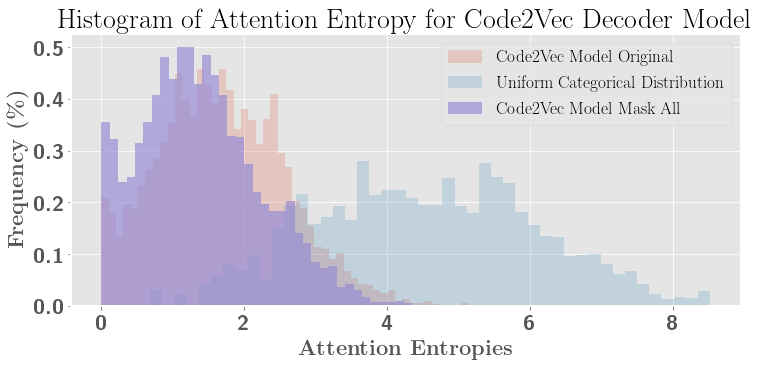
\includegraphics[width=0.8\linewidth]{ImagesCodeRelated/entropies_mask_all.png}
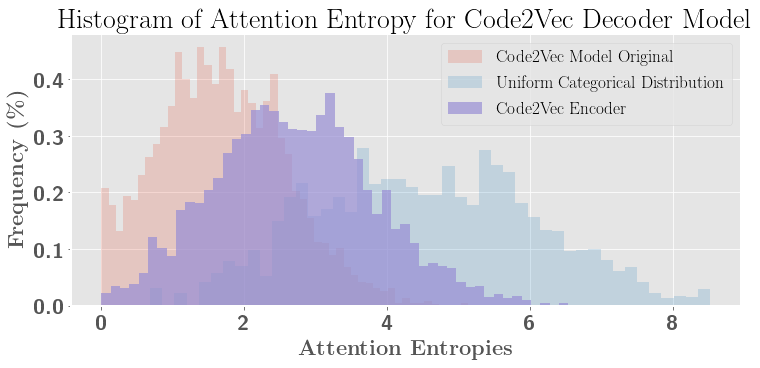
\includegraphics[width=0.8\linewidth]{ImagesCodeRelated/entropies_encoder.png}
\end{center}
\caption{all entropies}
\label{fig:all_entropies}
\end{figure}


\subsubsection{Analysis} % (fold)

Once again we investigated the performance of these models on the validation set, examining the entropies of both the masked models, on the validation dataset.

Noting the BLEU score and the lack of shift of the center of the entropies, it appears that losing coarguments, when the rest of the code is present, does not significantly impact the models behaviour.
There is a spike in the number of attentions with close to zero entropy, which could be explained by having informative codepaths involving coarguments, now being accessed more regularly at test time, but otherwise there is little change.

However, for the fully masked arguments we see alarge shift to even lower entropys, and greater mass closer to 0 entropy. In these cases it is likely the model is simply fitting to the paths it recognises, as the target nodes become less informative, and we start to see a performance of the model that starts to come close to the Rote Learner.

However, this experiment shows that by completely renaming all variables (including aliasing built-ins!), the model is still able to learn features from the paths of the source code themselves, suggesting that types of variables, and idiomatic expressions can add information, even in potentially very large syntax trees.


\begin{figure}
\begin{center}
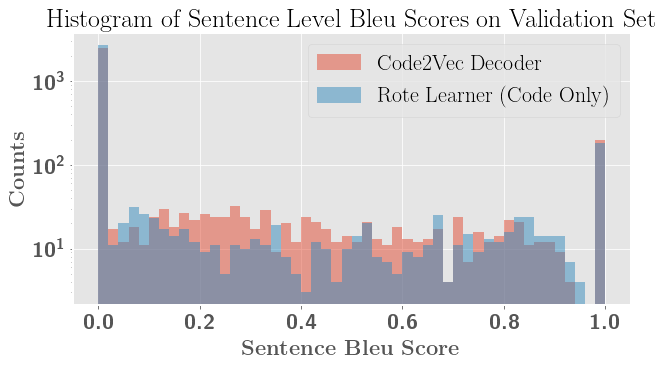
\includegraphics[width=0.75\linewidth]{ImagesCodeRelated/pretty_sentence_c2v.png}
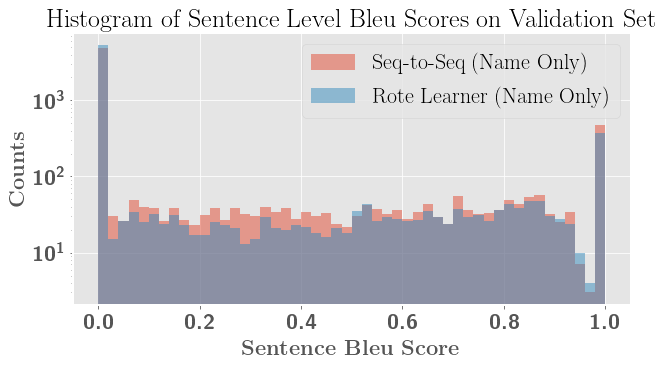
\includegraphics[width=.75\linewidth]{ImagesCodeRelated/pretty_sentence_bleu_s2s.png}
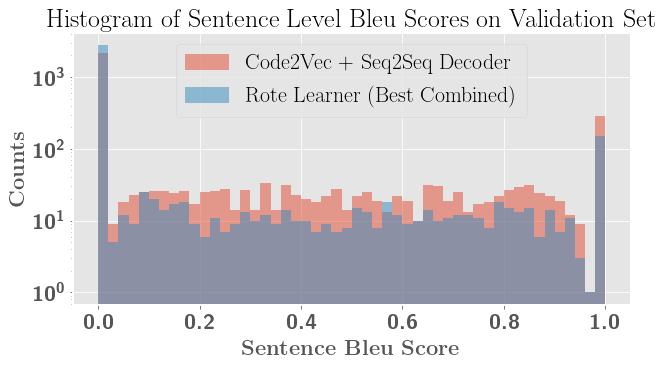
\includegraphics[width=.75\linewidth]{ImagesCodeRelated/pretty_sentence_bleu_c2e.png}
\end{center}
\caption{sentence bleu}
\label{fig:sentence_bleu}

\end{figure}

\begin{listing}[h!] 
\begin{center}

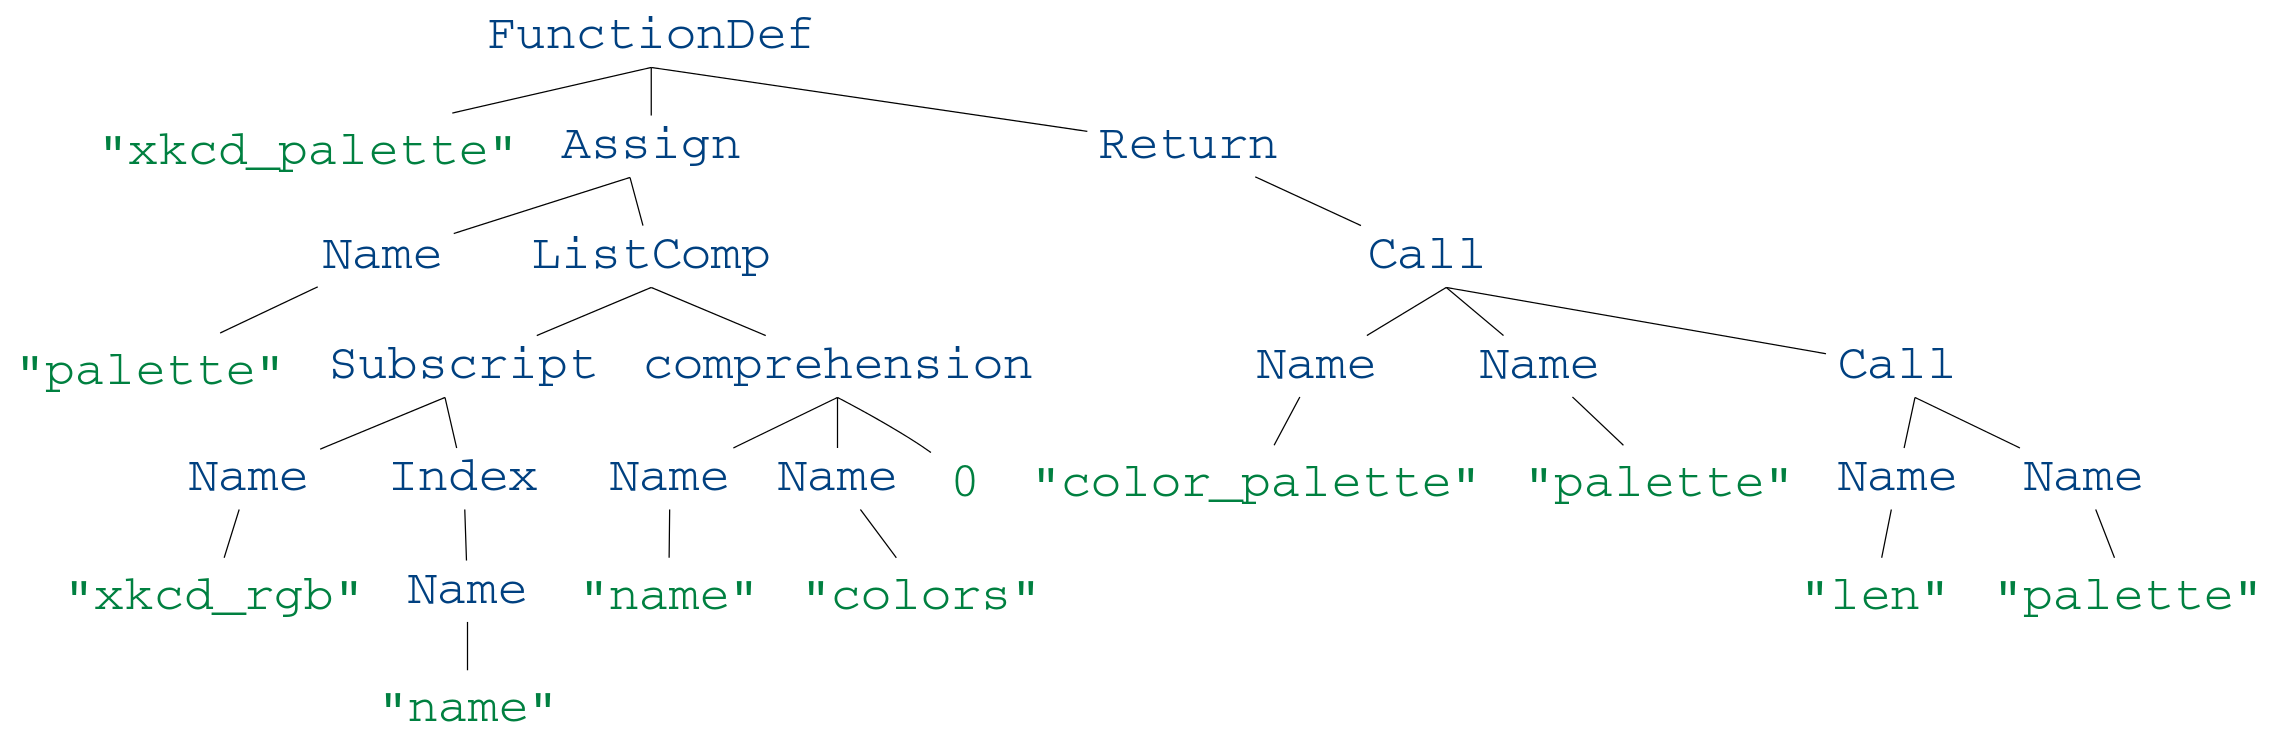
\includegraphics[width=\linewidth]{ImagesCodeRelated/xkcd_palette_strip.png}
\begin{minted}[]{python}
def xkcd_palette(colors):
    palette = [xkcd_rgb[name] for name in colors]
    return color_palette(palette, len(palette))

\end{minted}
\begin{tabular}{l}
\textbf{I}: \mintinline[]{python}{colors}\\
\textbf{D}: list of keys in the `` seaborn.xkcd\_rgb `` dictionary .\\
\textbf{P}: a list of data to read . if none , all other the first will be returned .\\
\end{tabular}
\end{center}
\end{listing}







\section{Investigating Combined Channels} % (fold)
\label{sec:investigating_combined_channels}


\subsection{Combined Code2Vec } % (fold)
\label{sub:combined_code2vec}

% subsection comparing_code2vec_to_baselines (end)

\subsubsection{Experiment Objective} % (fold)

Both the Seq-to-Seq models and Code2Vec Decoder models fundamentally look at different modalities of code when making their inference.
In this investigation we sought to investigate what could happen by combining these two modalities of information in the Code2Vec + Seq2Seq Decoder.

\subsubsection{Method \& Results} % (fold)

Given the nature of the code elements of this investigation, we continued with the Full Random-Split Library, and proceeded with the same format of investigation as outlined in previous sections. 
We ran the full neural models for 100 epochs, using the name only tokenizations for the human readable channel and the full unmasked paths for the code2vec encoder.

The results of these experiments are presented in Table \ref{table:code2vec_embed}. 
We report that the combined model surpasses both individual models achieving a BLEU of $28.7$ and $27.08$ on validation and test respectively. 
However, this is only making a small improvement on the Seq-to-Seq models, of about 2 points. 
This is at least partly down to the presence of (name, description) duplicate pairs in the dataset, which boosts both the performance of the Seq-to-Seq, and that of the rote learner.

It is interesting to note that the combined Rote Learner model performs worse when trying to learn on both modalities, achieving a score of $15.0$ annd $15.75$, which underperforms the name only model of $19.0$ and $19.68$ on validation and test.  


\begin{table}[h!]
\begin{center}
\begin{tabular}{ c | c | c  }
    Model                             & BLEU Validation  & BLEU Split     \\
    \hline
    Rote Learner  (code only)        & $ 11.84 \pm  0.16 $ & $ 12.62 \pm 0.12 $ \\
    Code2Vec Decoder                 & $ 18.94 $ & $ 18.13 $ \\
    % \hdashline
    % Code2Vec  (code only)             & $ 12.64199 $ & $ 12.80257 $ & \\
    \hline
    \hline
    Rote Learner  (name only)         & $ 19.04 \pm  0.35 $ & $ 19.69 \pm 0.28 $ \\
    Seq2Seq (name only)               & $ 26.40 $ & $ 25.40 $ \\
    % \hdashline
    % Seq2Seq  (name only)              & $ 15.94701 $ & $ 15.71091 $ & \\
    \hline
    \hline
    Rote Learner (combined)            & $ 15.02 \pm  0.45 $ & $ 15.76 \pm 0.30$ \\
    Code2Vec+ Seq-to-Seq Decoder       & $ 28.77 $ & $ 27.68 $ \\
    % \hdashline
    % Code2Vec  + Char to Seq           & $ 23.11775 $ & $ 22.37520 $ & \\
    % \hline
    % Model                             & BLEU Validation  & BLEU Split     \\
    % \hline
    % Rote Learner  (code only)        & $ 11.83875 \pm  0.15697 $ & $ 12.62479 \pm 0.12103 $ \\
    % Code2Vec Decoder                 & $ 18.93630 $ & $ 18.12909 $ \\
    % % \hdashline
    % % Code2Vec  (code only)             & $ 12.64199 $ & $ 12.80257 $ & \\
    % \hline
    % \hline
    % Rote Learner  (name only)         & $ 19.03534 \pm  0.35183 $ & $ 19.68826 \pm 0.28100 $ \\
    % Seq2Seq (name only)               & $ 26.39189 $ & $ 25.39841 $ \\
    % % \hdashline
    % % Seq2Seq  (name only)              & $ 15.94701 $ & $ 15.71091 $ & \\
    % \hline
    % \hline
    % Rote Learner (combined)            & $ 15.01764 \pm  0.44897 $ & $ 15.75528 \pm 0.29560 $ \\
    % Code2Vec+ Seq-to-Seq Decoder       & $ 28.76581 $ & $ 27.68100 $ \\
    % \hdashline
    % Code2Vec  + Char to Seq           & $ 23.11775 $ & $ 22.37520 $ & \\
    \hline
\end{tabular}
\caption {Investigate code2vec combined with seq to seq}
\label{table:code2vec_embed}
\end{center}
\end{table}

\subsubsection{Analysis} % (fold)


Analysis of the combined models largely followed the pattern of those in sections \ref{sec:investigating_the_computer_channel}, which involved looking at the entropies of the Code2Vec attention distributions and the sentence level BLEU scores, as evaluated over the whole of the validation set.

We found the unsurprisingly the Code2Vec + Seq to Seq Decoder model has a significantly wider distribution of entropies, centered around a higher point. 
This may partly be down to the fact that the model is now also learning from the highly informative variable name, and so depends less heavily on the specific code2vec paths. Nonetheless it still indicates the model is paying attention the codepaths when it makes its decisions.

This indicates why the model should outperform the Seq-to-Seq, but it given it is only a small improvement, it suggests that most of the performance gain comes from the name element of the data. 
Indeed, examining the distributions of sentence level BLEU scores, as visible in  \ref{fig:sentence_bleu}, suggests that te Seq-to-Seq model largely acts as a better Rote Learner, showing most of its improvements in the 1.0 scoring sentences. 
This is unsurprising given the number of duplicates of (name, description) pairs in this dataset.
Given the proximity of the BLEU scores for the Seq-to-Seq and Code2Vec + Seq-to-Seq scores, it is reasonable to assume a similar behavious is also occuring to some degree in the combined model.

% This is in agreement with the distribution of bleu scores in \ref{fig:sentence_bleu} v 

%  it is clear the availability of (name, description) duplicates helps both the name only learners, outperform the code only models ands suggests why the name only Rote Learner out performs the combined model. 

\section{Investigating the Library Split Dataset} % (fold)
\label{sec:analysis}

\subsubsection{Experiment Objective} % (fold)

Our final investigation sought to apply the most difficult test to our models, namely to investigate whether different modalities of code could help generate argument descriptions across completely differnet code bases and different authors.
This involved taking our strongest models and repeat them on our Full Library-Split Dataset.

\subsubsection{Method \& Results}  % (

The method of our investigations was as outlined above. In this case the models required significantly less training, plateauing their BLEU scores very early. We selected the best models that ran for at most 40 epochs. 
The results for each experiment is visible in Table \ref{table:split_datasets_embed}, with the hyperparameters presented in Table X.

We report that the neural model significantly struggled to learn the labelled translations on the library split datset.
The weakest models, the code only Code2Vec Decoders, scored BLEU scores of $0.89$ on both train and dev, very close to the code only Rote Learner score of   $ 1.01257 \pm  0.11410$, while the argument name models manage to achieve BLEU scores of about $1.5$ across both the Rote Learner and Seq-to-Seq models. 
Finally, the combined model of the Code2Dev + Seq-to-Seq model performs best, by a marginal amount, scoring  $ 1.85 $ and $ 1.59 $ across validation and test sets respectively,  outperforming the combined Rote Learner on both modalities byt about half a BLEU point.



\begin{table}[!ht]
\begin{center}
\begin{tabular}{ c | c | c }
    Model                             & BLEU Validation & BLEU Test \\
    \hline
    Rote Learner  (code only)         & $ 1.02 \pm  0.11 $ & $ 0.85 \pm 0.05 $ \\
    Code2Vec                          & $ 0.89 $ & $ 0.89 $ \\
    Code2Vec  (Mask Co-arguments)             & $ 0.67 $ & $ 0.67 $ \\
    Code2Vec  (Mask All)             & $ 0.69 $ & $ 0.71 $ \\
    \hline
    \hline
    Rote Learner  (name only)         & $ 1.44 \pm  0.17 $ & $ 1.36 \pm 0.06$ \\
    \hline
    Seq2Seq                             & &   \\
    - \textit{name only}              & $ 1.53 $ & $ 1.582$ \\
    - \textit{name + function name}      & $ 1.55 $ & $ 1.52 $ \\
    - \textit{name + co-argument names}         & $ 1.53 $ & $ 1.45$ \\   
    - \textit{name + function name +co-argument names}     & $ 1.51 $ & $ 1.48$ \\
    \hline
    \hline
    Rote Learner (combined)            & $ 1.23 \pm  0.169 $ & $ 1.157 \pm 0.101 $ \\
    Code2Vec  + Char to Seq            & $ 1.85 $ & $ 1.59 $ \\\\
    \hline


    % Model                             & BLEU Validation & BLEU Test \\
    % \hline
    % Rote Learner  (code only)         & $ 1.01257 \pm  0.11410 $ & $ 0.84707 \pm 0.04996 $ \\
    % Code2Vec                          & $ 0.88741 $ & $ 0.89466 $ \\
    % Code2Vec  (Mask Co-arguments)             & $ 0.66894 $ & $ 0.67366 $ \\
    % Code2Vec  (Mask All)             & $ 0.69457 $ & $ 0.71360 $ \\
    % \hline
    % \hline
    % Rote Learner  (name only)         & $ 1.43480 \pm  0.16744 $ & $ 1.36063 \pm 0.06452 $ \\
    % \hline
    % Seq2Seq                             & &   \\
    % - \textit{name only}              & $ 1.53474 $ & $ 1.58206 $ \\
    % - \textit{name + function name}      & $ 1.54843 $ & $ 1.52191 $ \\
    % - \textit{name + co-argument names}         & $ 1.53296 $ & $ 1.45225 $ \\   
    % - \textit{name + function name +co-argument names}     & $ 1.50983 $ & $ 1.48267 $ \\
    % \hline
    % \hline
    % Rote Learner (combined)            & $ 1.23201 \pm  0.16873 $ & $ 1.15672 \pm 0.10083 $ \\
    % Code2Vec  + Char to Seq            & $ 1.84887 $ & $ 1.58697 $ \\\\
    \hline
\end{tabular}
\caption {Investigate split datasets}
\label{table:split_datasets_embed}
\end{center}
\end{table}




\subsubsection{Analysis}

These results at first glance seem to indicate that the neural models can perform no better in generalised translation than the overfitting Rote Learner models.
However these low BLEU scores give little indication to the type of translations that are being generated.
To investigate the quality of these translations we examined a random sample of translations from both the Rote Learner and the Code2Vec models. 
A random sample are shown in Table \ref{tab:lib_split}.

In these we see very little overlap, though the translations make grammatical sense. 
In particular the types of descriptions generated appear shorter and more general than their counterparts with the Rote Learner, but both generally have a poor alignment with the true description.

% Although we see a very low ngram overlap,
% 1)  descriptions of the neural models seem plausible, and certainly less repeated and specific that Rote Learner.
% 2) (However,) looking at the one word overlap of the the models we see the following distributions.
% Searching for direct repeats of translations we find that X of the validation sentences are found in the training, indicating /not invdicating overfitting.

These low BLEU scores, despite grammatical sounding descriptions, lead us to the biggest problem with this task.
Generalisation across code documentation is difficult when code is written by different authors, with different contexts and conventions. 
Although related work in section X demonstrates that idioms and patterns in code do exist, we are fundamentally hampered by the both the variance of code between libraries and variation of the target language that we aim to generate when we split between libraries.
Codebases develop idioms and name conventions within libraries, and often have a context when it comes the language used in descriptions. 
Unlike in many words in the real world, descriptions of code artefacts are almost always metaphorical (for instance "colours", instead of "list of strings"),  and therefire different libraries are under no obligation to use the same language, or even vocabularies when referring to the same underlying code objects. 

For instance a list of strings could just as easily by a \mintinline[]{python}{x_axis_labels} or \mintinline[]{python}{song_categories}, but generating language surround the second example may be difficult without training examples without example of the relevant context.
 In the abstract the model may be able to infer something general, such as the type, but again idiomatic use of the code would need to be provided for this.

This lack of context and vocabulary, both with code and text, seems to be the case with our datasets.
We investigated how the different train set and validation set description vocabularies varied between the Random-Split and Library-Split Datasets after tokenization, and found that the in our Library Split dataset, the vocabularies of our training set are reduced by over 10\%, compared to a Random Split. 
Furthermore, we also found that after tokenization 16\% of the words in our validation set vocabulary do not even appar in the training set - even though these are not "UNK" tokens. This is almost a fourfold increase compared to the Random Split dataset.

\begin{table}
    \begin{center}
        \begin{tabular}{c c c}
           \hline
            & Random Split & Library Split \\
            \hline
            Tokenized Train Description Vocab Size    & 5249  &  4701 \\
            Tokenize Valid Description Vocab Size    & 3012  &  2866 \\
            \% of Tok. Valid Vocab not in Tok. Train Vocab                & 4.1\% &  15.8\% \\
            \hline
            \% of $<$UNK$>$ path elements in Train          &  37.4\%  &  32.4 \%   \\
            \% of $<$UNK$>$ path elements in Validation     &  37.5\%  &  57.4\% \\
            \% of $<$UNK$>$ terminal nodes in Train         &  12.3\%  &  8.8\%  \\ 
            \% of $<$UNK$>$ terminal nodes in Validation    &  14.7\% &  44.9\% \\   
            \hline
        \end{tabular}
    \end{center}
    \caption{A table showing the change in the actual vocabulary of the argument descriptions, and also change in out-of-vocabulary tokens, for different library splits.}
    \label{tab:vocabsplit}
\end{table}



This behaviour is even worse when it comes to the code paths.
Unlie the vocabulary for descriptions, the the vocabulary for code paths is set entirely by the training set - there are no Glove preembeddings of paths to help!
As a results we found that the fraction of codepaths with "<UNK>" path component in the validation set rose from 38\% to 58\%, and "<UNK>" terminal nodes ran from 15\% to 45\%. 
These large increases further explain why, even on a general level looking at the computer channel, our Code2Vec models struggled to generalise. A summary of these results in presented in Table \ref{tab:vocabsplit}

This work shows how challenging it is to generalise code across repository. Syntax trees are vast and diverse, which poses a problem for vocabularies, even if only taking a small subsection of the tree. 
Furthermore, the language thats used is necessarily different and metaphorical, which leads to fitting on training that fails to generalise.
It is possible that other tokenizations of the source code on this dataset may prove more informative in future, which may be a promising path of future investigation.




\begin{table}[ht]

    \centering

\makebox[\linewidth][c]{
    \begin{tabular}{l}

    \hline
    \textbf{Argument}: \mintinline[]{python}{kind}\\
    \textbf{Description}: interpolation mode for the frequency estimator . see :\\
     `` scipy.interpolate.interp1d `` for valid settings .\\
    \textbf{Rote Learner}:   sample weights . \\
    \textbf{Code2Vec Decoder}: maximum number of iterations to use .\\
    \\
    
    \textbf{A}: \mintinline[]{python}{query}\\
    \textbf{D}: the query parameters , as a dictionary or as an iterable of key-value pairs .\\
    \textbf{C2V}: the name of the $<$UNK$>$ .\\
    \textbf{RL}: int , or tuple of $<$UNK$>$ , or tuple of 3 tuples of 2 ints . - if int : the same \\
    symmetric cropping is applied to depth , height , and width . - if tuple of 3 ints : interpreted \\
    as two different symmetric cropping values for depth , height , and width : ` ( $<$UNK$>$ , $<$UNK$>$ , \\
     $<$UNK$>$ ) ` . - if tuple of 3 tuples of 2 ints : interpreted as ` ( ( $<$UNK$>$ , $<$UNK$>$ ) , ( $<$UNK$>$ ,\\
      $<$UNK$>$ ) , ( $<$UNK$>$ , $<$UNK$>$ ) ) ` \\
    \\
    
    \textbf{A}: \mintinline[]{python}{obj}\\
    \textbf{D}: an object .\\
    \textbf{C2V}: a list of tensors to be used .\\
    \textbf{RL}: depth multiplier for $<$UNK$>$ convolution ( also called the resolution multiplier ) \\
    \\
    
    \textbf{A}: \mintinline[]{python}{networks}\\
    \textbf{D}: list of network names or ids to attach the containers to .\\
    \textbf{C2V}: the number of jobs to use .\\
    \textbf{RL}: copy data from inputs . only affects $<$UNK$>$ / 2d $<$UNK$>$ input \\
    \\
    
    \textbf{A}: \mintinline[]{python}{G}\\
    \textbf{D}: a networkx graph\\
    \textbf{C2V}: the $<$UNK$>$ object to use .\\
    \textbf{RL}: \ ` $<$UNK$>$ ` . \\

    \hline

    \hline
    \end{tabular}
    }

    \caption{A sample of translations on the Library Split Dataset, in this case with the Code2Vec Decoder model}
    \label{tab:lib_split}
\end{table}




% \chapter{Analysis}
\label{analysis}
\chapter{Conclusions and Further Work}
\label{chapterlabel4}


\section{Conclusions}

At the start of this report we sought to address four questions in our problem formuation:

\begin{tight_enumerate}
    \item whether reasonable summaries can be generated from just lexical names in the function signature?
    \item whether reasonable summaries can be generated from the functions abstract syntax tree, without the lexical data?
    \item whether these models, can be combined in a way that surpasses each individually?
    \item whether such models can work both in an `in-project' setting and an `out-project setting'?
\end{tight_enumerate}

Over the course of this report we have provided evidence to address the answers to each of these questions. 

First we conclude that reasonable summaries \textit{can} be generated from just names in the function signature. 
In particular we have shown that reasonable descriptions can be generated from just the argument name, by looking at its the character substructure. Operating on our Reduced Random Split Dataset, our Seq2Seq model achieves test BLEU score of 12.72 - surpassing a Rote Learner that regurgitates memorised descriptions for similar names.  
We can also conclude that other aspects of the signature, such as corguments and the function name, also prove informative, since they boost perfomance in our Rote Learner and in most of our Seq2Seq cases. 
This highlights the informative power of the function signature, and the names that are chosen within it.

Secondly we conclude that reasonable summaries \textit{can} be generated from just the AST, without any reference to the name of the argument. 
By using the \textit{variable path-context} (VPC) representation, we showed that Rote Learner that memorised descriptions and matched VPCs could achieve a BLEU score of 12.61 on our Full Random-Split Dataset. This was then ourperformed by our neural Code2Vec Decoder, which achieved a test BLEU score of 18.13, generating original descriptions. 
We demonstrate that this model can outperform the Rote Learner despite partial or full occlusion of the names of objects in the AST, achieving BLEU scores of 16.94 and 13.07 respectively.

Thirdly we conclude that combining our two different modalities results in a stronger model than either of the two individually. By simply each individually concatenated encoded vectors our Code2Vec + Seq2Seq model surpasses individual models by 2 BLEU points on the Full Random-Split Dataset.

Finally our investigation to our the last question to proves inconclusive. We notice a significantly worse performance of our models on the `out-project' setting, though they generate sentences with fluency. We demonstrate that due to tokenizations of the dataset, a large fraction of test-set features are rendered out-of-vocabulary in this setting, raising the question of whether the models or the tokenizations are the problem in this case. 

% This just dumps some pseudolatin in so you can see some text in place.
\section{Limitations \& Critique}

In the course of the above investigations, we encountered a number of limitations that affected our progress.

\paragraph{Dataset} 
First and foremost, we noted that the composition of our dataset disproportionately originates from a single source - 41\% of our arguments are from \mintinline[]{python}{tensorflow}. This proved less problematic for Random Split Dataset but in a Library Split setting this accounts for most of the training data - which also includes \mintinline[]{python}{scipy} and \mintinline[]{python}{numpy}. Therefore the variance of our training set would have been much reduced, hindering our investigation into Library Split Data.

Secondly, although the size of our Full Datasets are comparable to others\footnote{such as the Stack Overflow SQL dataset}, our Reduced Dataset are arguably too small for our neural methods in character-level tasks. In particular this small dataset may explain the overfitting in these tasks, and should have ideally have been bigger in these investigations, or subject to data augmentation.

\paragraph{Metric} 
A major limitation of our overall investigation is a lack of automatic metrics for assessing description quality. Without skilled human intervention in reading the source code, it is hard to evaluate whether an argument description is true, even if the n-gram precisions (as measure by BLEU) is poor. In machine translation, often multiple synonymous reference sentences are provided to improve the validity of n-gram precision \citep{papineni_bleu_2001}, but in our case no multiple translations exist. Automating a measure of evaluating description would greatly assist in-depth analysis of where the models fail.

\paragraph{Resources} 

Finally a limitation of our overall investigation is our resources available. Since we aimed to fit all our work on one GPU, we were constrained to use a limited vocabulary of paths, terminal nodes. Increasing these would likely help in both Random Split and Library Split contexts

\section{Further Work}

* Seq2Seq
* 

% \chapter{Note to Matko}
\label{baselines_note}

\textit{
This is a note to explain the current situation of the project, and to decide what might need doing in the last few weeks of the project. 
I'm aware I have a lot of different ways of chopping the data set, and differnet models, so there is potential to investigate a lot.
As such this note is just to clarify thoughts for this last week.}

\section{The Dataset (A Reminder)} % (fold)
\label{sec:the_dataset}

The raw dataset is the set of all functions that obey the \mintinline{python}{numpy} or \mintinline{python}{google} standard of docstrings, from top 300 libraries as available on \mintinline{python}{pip}. 
These were collected by writing an extension to the \mintinline{python}{sphinx} documentation generator, which is the industry standard for automatic code documentation.

In terms of the amount of data collected:
\begin{itemize}
    \item 133 libraries contributied to dataset
    \item 12,079 function definitions were collected
    \item 39,205 (argument, description) pairs were collected
\end{itemize}

In examining this data, I found the data to be highly biased towards scientific libraries, and also within these libraries, many functions containing identical pairs of (argument, description). 
The reasons for this are simple: 
\begin{enumerate}
    \item Scientific libraries have vast API's, so need good documentation for inputs and outputs.
    \item Some the arguments for these apis are likely to be identical, leading coders to copy them. 
    E.G \mintinline{python}{name} for a tensor in \mintinline{python}{tensorflow}.
\end{enumerate} 

\subsection{Data Set Investigation} % (fold)
\label{ssub:datasetinvestigation}

In the report I aim present an investigation of the dataset from a statistical point of view, but also a qualitative point of view.
I want to both know: 
\begin{itemize}
    \item Statistics about natural language: eg - variable names, description lengths, uniqueness of variable names and (variable, description) pairs, vocabulary size
    \item Statistics about code and syntax trees: eg - tree sizes, paths, uniquenesses of paths
    \item Clustering of natural language: eg how similar are the libraries? is there a distinction between scientific and other libraries, based on either description, or argument name, or names of source code. How much `bias' is there in the dataset?
\end{itemize}

I have done the first two investigations, on Jupyter notebooks but I am yet to do the third.

The results of the the first two investigations I will paste here fully in due time, but the in summary I noticed that there are a often arguments have identical descriptions, even if they come from different functions with different code. 
This allows a dumb learner that effectively just memorizes previous descriptions and names, to perform with  significant hit rate.  
As a result, I created various datasets that effectively capped the number of duplicate (argument, description) pairs.

\begin{center}
\begin{tabular}{|| c | c | c ||}
  \hline
   Name of DataSet & No of Duplicates & Data Set Size \\
  \hline
   UnsplitND1 & 0 & 22917 \\
   UnsplitND2 & 1 & 28771 \\
   UnsplitND3 & 2 & 31063 \\
   UnsplitND4 & 3 & 32487 \\
   UnsplitND5 & 4 & 33398 \\
   UnsplitNDX & 9 & 35551 \\
   Unsplit    & NA & 39205\\ 
  \hline
\end{tabular}
\end{center}

Finally I also had the option of choosing whether to divide my dataset along repository lines for training and validation/test, or whetehr to keep the function together. 
That is: should code from a the test and validation set be from different libraries as the train set. 

I have so far prepared one of these data sets but I have not prepared the no duplicates set.

\begin{center}
\begin{tabular}{|| c | c | c ||}
  \hline
   Name of DataSet & No of Duplicates & Data Set Size \\
  \hline
   Split    & NA & 39205\\ 
  \hline
\end{tabular}
\end{center}

\section{Hashtable Baselines} % (fold)
\label{sub:hashtable_baseline}

All hashtable baseline models shared a common idea: identify a feature to match, and randomly choose a stored description from the training set, whose data matches this feature. 
Although this led to several differnt models (largely based on what consitutes a match, and which features are available to the model), this baseline proved vital to compare to the LSTM models, as it indicated the limits of "overfitting". 
Surpassing these models should indicat that something generalizable in the data has been learnt.

\subsection{Natural Language Lookup} % (fold)
\label{sub:natural_language_lookup}
When dealing with natural language text data, the model attempted to find the largest overlapping n-character-gram, and drew randomly from the set of matched descriptions.

There were four available tokenizations of the data that only pertained to the natural language of the function signiature, and they were concatenated with unique character separators, to form long strings for the lookup table

% subsection natural_language_lookup (end)

\begin{enumerate}
    \item the argument name
    \item the argument name + the function name
    \item the argument name + the names of the other arguments
    \item the argument name + the function name + the names of the other arguments
\end{enumerate}

\subsection{Code Path Lookup} % (fold)
\label{sub:code_path_lookup}

In a similar spirit, the hashtable model aims to memorise `code paths' as defined in the code2vec paper, and then for each test point, return a randomly chosen description from the set of best matches.

In this case what constitutes a match can vary, so a delineation is based on whether full paths (`hard') need to be matched, or subpaths can be matched (`soft')
\begin{enumerate}
    \item \textit{hardest} - chose from the set of descriptions which have the most matching full paths.
    \item \textit{hard} - chose from the set of descriptions in proportion to the number of matching full paths.
    \item \textit{soft} - chose from the set of descriptions with the greatest matched subpaths.
    \item \textit{softest} - chose from the set of descriptions  with proportion to the number of matching subpaths.
\end{enumerate}

Of these, I run into memory issues with the soft (for some reason), and still need to run it on the full datasets. 
% subsection code_path_lookup (end)

\subsection{Combined Lookup} % (fold)
\label{sub:combined_lookup}

To do a combined lookup, simply add the two possible sets of descriptions together, before randomly choosing. 

% subsection combined_lookup_and_results (end)

\subsection{Results} % (fold)
\label{sub:results}

In terms of results, I first ran the hashtable baseline with just text and different tokenizations. If you remove the duplicates the model performs significantly worse.

Then I have on the same dataset run the code sections.

I found this.



\section{Neural Models} % (fold)
\label{sec:neural_models}

\subsection{CharToWord Seq to Seq} % (fold)
\label{sub:chartoword_seq_to_seq}

So far this model has failed to beat the baseline. At best it seems capable of matching it. My theories as to why this is:
 \begin{enumerate}
     \item Unlike in sentences where words depend on each other in a confusing syntactic patterns with long range dpependencies, words in a sentence have shorter range dependencies, often neighbouring matters the most or sub phrases.
     \item Therefore ngram overlap is a very significant feature - indeed its what humans look for when trying to work out what variables are
 \end{enumerate}

 I expected cases such as including functon name or other arguments to hurt performance, and it would add a lot of noise. This turned out not to be the case. Perhaps the benchmark's advantage of always being able to generate well formed descriptions also came into play.

 At any rate I have a significant number of experiments here, with the different tokenizations of the data, and different types of seq to seq model (attention no attention, bidirectional or not, trainable embeddings or not), that i could write about.

 \subsection{CodeToVec to Seq} % (fold)
 \label{sub:codetovec}

 This model is an implementation of thde code2vec paper 


 \subsection{To Do} % (fold)
 \label{sub:to_do}
 
 \begin{enumerate}
   \item split data set and run experiments
   \item rename variables in ast \& run (2 tokenizations)
   \item hyperparam sweep \& tune
   \item dropout for code 2 vec
   \item ?? use source code in bag of source code words model??
   \item use all paths (like code 2 vec paper)
   \item run hashtable baseline on other datasets
 \end{enumerate}
 % subsection to_do (end)
 









% The \appendix command resets the chapter counter, and changes the chapter numbering scheme to capital letters.
%\chapter{Appendices}
\addcontentsline{toc}{chapter}{Appendices}

\appendix

\chapter{Dataset Examples}
\label{example_datapoint}
% Figure \ref{lst:single_point} shows a real example of a datapoint in YAML markup. 
% Different parts of the data were used in the investigation.
\begin{listing}[h!]
\begin{minted}[]{yaml}
-   arg_name: tensors                                 # argument name: STRING
    arg_desc: ' a list of variable or op tensors.'    # argument description: STRING
    arg_type: null                                    # argument type: STRING or NULL
    args: [tensors, prefix]                           # list of arguments: LIST of STRING
    arg_info:                                         # info on other arguments: DICT of DICT
        prefix: 
            desc: ' An optional prefix for the summary names.' 
            type: null
    filename: /tensorflow/contrib/slim/python/slim/summaries.py  # filename: STRING
    name: add_zero_fraction_summaries                 # function name: STRING 
    sig: (tensors, prefix=None)                       # function signature: STRING
    pkg: tensorflow                                   # library: STRING  
    src: |                                            # source code: STRING 
      def add_zero_fraction_summaries(tensors, prefix=None):
        """Adds a scalar zero-fraction summary for each of the given tensors.
  
        Args:
          tensors: a list of variable or op tensors.
          prefix: An optional prefix for the summary names.
  
        Returns:
          A list of scalar `Tensors` of type `string` whose contents are the
          serialized `Summary` protocol buffer.
        """
        summary_ops = []
        for tensor in tensors:
          summary_ops.append(add_zero_fraction_summary(tensor, prefix=prefix))
        return summary_ops
    docstring: |                                      # sphinx annotated docstring: STRING 
      Adds a scalar zero-fraction summary for each of the given tensors.

      :param tensors: a list of variable or op tensors.
      :param prefix: An optional prefix for the summary names.

      :returns: A list of scalar `Tensors` of type `string` whose contents are the
                 serialized `Summary` protocol buffer.
\end{minted}
     \caption{Real example of a single data point, with all metadata. The docstring in the source has been elided for brevity}
     \label{lst:single_point}
\end{listing}

\begin{table}[h]
    \begin{center}
    \begin{tabular}{c | c | c }       
 Arg. Name (Total) & Top 5 Descriptions & Count\\
\hline
name   (1917) &  a name for the operation (optional).                                & 1057\\
&  optional op name.                                                   & 69 \\
&  an optional variable\_scope name.                                    & 41 \\
&  a name for this operation (optional).                               & 37 \\
&  a string, the name of the layer.                                    & 31 \\

\\
\hline
x   (439) &  tensor or variable.                                                 & 32 \\
&  a tensor or variable.                                               & 17 \\
&  `bfloat16`, `half`, `float32`, `float64`, `complex64`, `com[...]   & 14 \\
&  numeric `tensor`.                                                   & 12 \\
&  array or sequence containing the data                               & 10 \\

 \\
\hline
kwargs   (303) &  additional keyword arguments which will be passed to the ap[...]   & 12 \\
& optional arguments that ``request`` takes.                          & 11 \\
& standard layer keyword arguments.                                   & 8 \\
& additional properties to be set on the :class:`~.google.clo[...]   & 7 \\
& keyword arguments to pass to base method.                           & 5 \\

\\
\hline
axis   (263)  &  axis to broadcast over                                              & 14 \\
& the dimensions to reduce. if `none` (the default), reduces [...]   & 7 \\
& the index or the name of the axis. 0 is equivalent to none [...]   & 4 \\
& a `tensor` of type `int64`.                                         & 4 \\
& the axis or axes that were summed.                                  & 4 \\

\\
\hline
dtype   (260) &  a `tf.dtype`.                                                       & 11 \\
& the data type. only floating point types are supported.             & 8 \\
& default data type for internal matrices. set to np.float32 [...]   & 7 \\
& the type of the output.                                             & 6 \\
& overrides the data type of the result.                              & 6 \\


    \end{tabular}
        \caption { A table of the count and frequency of function names of the variables as they feature in the raw dataset. 
        These can be either due to the repetition of function name throughout libraries, or by one argument contributing many functions }
    \label{table:descriptions_for_names} 
    \end{center}
\end{table}

\begin{table}[h]
    \begin{center}
    \begin{tabular}{c | c | c | c | c | c | c | c | c  }       

 Variable Name &name         & &  x            &  & kwargs   & &  axis    \\
\hline
Top 5 Libraries  &tensorflow         & 1654     & tensorflow    & 300       & tensorflow    & 62       & tensorflow    & 85 \\
&google             & 51       & matplotlib    & 43       & google        & 47       & pandas        & 61       \\
&tflearn            & 50       & scipy         & 35       & dask          & 23       & scipy         & 54       \\
&external           & 14       & tflearn       & 12       & mir\_eval     & 21       & dask          & 20       \\ 
&absl               & 13       & dask          & 9        & librosa       & 18       & librosa       & 17       \\



    \end{tabular}
        \caption { A table of the count and frequency of function names of the variables as they feature in the raw dataset. 
        These can be either due to the repetition of function name throughout libraries, or by one argument contributing many functions }
    \label{table:packages_for_names} 
    \end{center}
\end{table} 
\chapter{Rote Learner Algorithms}


\begin{algorithm}
    \caption{The NGram Overlap Matching algorithm }
    \label{alg:ngram_overlap}
    \begin{algorithmic}
        \Procedure{BestMatchingSet}{$test, training\_points$} %\Comment{Find best matching set for test argument $t$ }
        % \State $c \gets \text{getCharSequence}(test\_point) $
       
        % \State $n \gets \text{characterLength}(s)$
        % \While {$n > 0$}  \Comment{Start with longest overlap}
        %     \State ${M} = \textbf{[ ]}$
        %     \State ${S} \gets \text{getNCharacterGrams}(s, n)$
        %     \For {$t \textbf{ in } training\_points$}
        %         % \State $d \gets \text{getCharSequence}(t) $
        %         \State ${T} \gets \text{getNCharacterGrams}(t, n)$
        %         \For {$\textbf{each in }  {S} \cap {T}$}
        %             \State $ {M} \gets  {M} + \text{[ }t\text{ ]}$
        %              \Comment{There may be more than one overlap}
        %         \EndFor
        %     \EndFor
        %     \If {${M} \ne \textbf{[ ]}$}
        %         \State $\textbf{return } {M}$
        %     % \Else
        %     \EndIf
        %     \State $n \gets n - 1$
        % \EndWhile \Comment{If no overlap, choose from all training points}

        \State \text{toCharSequence} $\gets$ lambda(x)\{x[`character\_sequence']\}
        \State $M \gets \text{LargestOverlappingSubsequence}(test, training\_points, \text{toCharSequence})$
        \State $\textbf{return } M$

        \EndProcedure

    \end{algorithmic}
\hrulefill

    \begin{algorithmic}
        \Procedure{LargestOverlappingSubsequence}{$y\_data, X\_data$, toSequence} %\Comment{Find best matching set for test argument $t$ }
        % \State $c \gets \text{getCharSequence}(test\_point) $
        
        \State $y \gets \text{toSequence}(y\_data)$
        \State $l \gets \text{length}(y)$
        \For {$n \text{ in } \{l, l-1 ..., 1\}$}  \Comment{Start with longest overlap}
            \State ${C} = \textbf{[ ]}$
            \State ${N} \gets \text{getSubSequences}(y, n)$
            \For {$x\_data \textbf{ in } X$}
                \State $x \gets \text{toSequence}(x\_data)$
                % \State $d \gets \text{getCharSequence}(t) $
                \State ${M} \gets \text{getSubSequences}(x, n)$
                \For {$\textbf{each in }  {S} \cap {T}$}
                    \State $ {C} \gets  {C} + \text{[ } x\_data \text{ ]}$
                     \Comment{There may be more than one overlap}
                \EndFor
            \EndFor
            \If {${C} \ne \textbf{[ ]}$}
                \State $\textbf{return } {M}$
            \EndIf
        \EndFor \Comment{If no overlap, return all}
        \State $\textbf{return } X\_data$
        \EndProcedure
    \end{algorithmic}
\hrulefill

    \begin{algorithmic}
        \Procedure{getSubSequences}{$x, n$} \Comment{Get all subsequences from x, length n} 
        \State l = \text{length}($x$)
        \State $\textbf{return } [x[i:i+n] \text{ for i in } \{0,...,l-n+1\} ]$

        \EndProcedure
    \end{algorithmic}


\end{algorithm}



\begin{algorithm}
    \caption{The Path-Context Matching algorithms (Max and Proportional) }
    \label{alg:context_algorithm}
    \begin{algorithmic}
        \Procedure{BestMatchingSetProportional}{$test, training\_points$} %\Comment{Find best matching set for test argument $t$ }
        % \State $c \gets \text{getCharSequence}(test\_point) $
        \State ${M} = \text{getPathContextOverlap}(test, training\_points)$
        \State $\textbf{return } M$
        \EndProcedure
    \end{algorithmic}
    \hrulefill
    \begin{algorithmic}
        \Procedure{BestMatchingSetMax}{$test, training\_points$} %\Comment{Find best matching set for test argument $t$ }
        % \State $c \gets \text{getCharSequence}(test\_point) $
        \State ${M} = \text{getPathContextOverlap}(test, training\_points)$
        \State $\textbf{return } \text{mostFrequent}(M)$
        \EndProcedure
    \end{algorithmic}
    \hrulefill
    \begin{algorithmic}
        \Procedure{getPathContextOverlap}{$s, training\_points$} %\Comment{Find best matching set for test argument $t$ }
        % \State $c \gets \text{getCharSequence}(test\_point) $
        \State ${M} = \textbf{[ ]}$
        \State ${S} \gets \text{getPathContexts}(s)$
        \For {$t \textbf{ in } training\_points$}
            \State ${T} \gets \text{getPathContexts}(t)$
                \For {$\textbf{each in }  {S} \cap {T}$}
                    \State $ {M} \gets  {M} + \text{[ }t\text{ ]}$
                     
                \EndFor
        \EndFor
        \State $\textbf{return } M$
        \EndProcedure
    \end{algorithmic}
    \hrulefill
    \begin{algorithmic}
        \Procedure{getPathContexts}{$x$} %\Comment{Find best  
        \State $\textbf{return } x$[`path\_contexts']
        \EndProcedure
    \end{algorithmic}

\end{algorithm}



\begin{algorithm}
    \caption{The SubContext Matching algorithms (Max and Proportional)}



    \label{alg:sub_context_algorithm}
    \begin{algorithmic}
        \Procedure{BestMatchingSetProportional}{$test, training\_points$} %\Comment{Find best matching set for test argument $t$ }
        % \State $c \gets \text{getCharSequence}(test\_point) $
        \State ${M} = \text{getSubPathContextOverlap}(test, training\_points)$
        \State $\textbf{return } M$
        \EndProcedure
    \end{algorithmic}
    \hrulefill
    \begin{algorithmic}
        \Procedure{BestMatchingSetMax}{$test, training\_points$} %\Comment{Find best matching set for test argument $t$ }
        % \State $c \gets \text{getCharSequence}(test\_point) $
        \State ${M} = \text{getSubPathContextOverlap}(test, training\_points)$
        \State $\textbf{return } \text{mostFrequent}(M)$
        \EndProcedure
    \end{algorithmic}
    \hrulefill

    \begin{algorithmic}
        \Procedure{getSubPathContextOverlap}{$s, training\_points$} %\Comment{Find best matching set for test argument $t$ }
        % \State $c \gets \text{getCharSequence}(test\_point) $
        \State ${M} \gets \textbf{[ ]}$
        \State ${S} \gets \text{getPathContexts}(s)$
        \State \text{toPathContextSequence} $\gets$ lambda(x)\{split(x[`path\_context'])\}

        \State ${X\_data} \gets \text{flattenPathContexts}(training\_points)$

        \For {$s \textbf{ in } S$}
            \State $m \gets \text{LargestOverlappingSubsequence}(s, X\_data$, toPathContextSequence) 
            \State $M \gets M + m$

        \EndFor
        \State $\textbf{return } M$
        \EndProcedure
    \end{algorithmic}
    \hrulefill
    \begin{algorithmic}
        \Procedure{flattenPathContexts}{$all\_xs$} %\Comment{Find best ma
        \State {$flat \gets \text{[ ]}$}
        \For {$x \textbf{ in } all\_xs$}
            \For {$p \textbf{ in } x\text{[`path\_contexts']}$} 
                \State $y \gets x$
                \State $y[`path\_contexts'] \gets [p]$
                \State $flat \gets flat + [y]$
            \EndFor
        \EndFor

        % \State $\textbf{return } x$[`path\_contexts']
        \State $\textbf{return }flat$
        \EndProcedure
    \end{algorithmic}
\end{algorithm}





    % \begin{algorithmic}
    %     \Procedure{BestMatchingSet}{$s, training\_points$, mode} %\Comment{Find best matching set for test argument $t$ }
    %     % \State $c \gets \text{getCharSequence}(test\_point) $
    %     \State ${M} = \textbf{[ ]}$
    %     \State ${S} \gets \text{getPathContextsAsSequence}(s)$
    %     \For {$t \textbf{ in } training\_points$}
    %         \State ${T} \gets \text{getPathContextsAsSquence}(t)$
    %             \For {$\textbf{each in }  {S} \cap {T}$}
    %                 \State $ {M} \gets  {M} + \text{[ }t\text{ ]}$
                     
    %             \EndFor
    %     \EndFor
    %     \If {{mode} = \text{`prop'}}
    %         \State $\textbf{return } M$
    %     \ElsIf {{mode} = \text{`max'}}
    %         \State $\textbf{return } \text{mostFrequent}(M)$
    %     \EndIf
    %     \EndProcedure
    % \end{algorithmic}





    % \begin{algorithmic}
    %     \Procedure{BestMatchingSet}{$s, training\_points$} 
    %     \State $n \gets \text{characterLength}(s)$
    %     \While {$n > 0$}  \Comment{Start with longest overlap}
    %         \State ${M} = \textbf{[ ]}$
    %         \State ${S} \gets \text{getPathContextsAsSequence}(s, n)$
    %         \For {$t \textbf{ in } training\_points$}
    %             \State ${T} \gets \text{getPathContextsAsSequence}(t, n)$
    %             \For {$\textbf{each in }  {S} \cap {T}$}
    %                 \State $ {M} \gets  {M} + \text{[ }t\text{ ]}$
    %                  \Comment{There may be more than one overlap}
    %             \EndFor
    %         \EndFor
    %         \If {${M} \ne \textbf{[ ]}$}
    %             \State $\textbf{return } {M}$
    %         % \Else
    %         \EndIf
    %         \State $n \gets n - 1$
    %     \EndWhile \Comment{If no overlap, choose from all training points}
    %     \State $\textbf{return } training\_points$

    %     \EndProcedure
    % \end{algorithmic}



\chapter{Model Hyperparameters}
\label{Model Hyperparameters}

The hyperparameters of the best model for each experiment are presented in this section for ease of replication.


\begin{table}[h!]
\begin{center}
\begin{tabular}{ c | c | c  }
    \textbf{Model}                           {}  & \textbf{Hyperparameter}  & \textbf{Value}    \\
    \hline
    -                                 & vocabulary size            & $40,000$ \\
    \hline
    Rote Learner                      & feature                    & \textit{n}-character-gram overlap \\
                                      % & samples                           & $50$  \\
    \hline
    Seq to Seq                        & learning rate              & $0.001$         \\
                                      & batch size                 & $128$           \\
                                      & lstm size                  & $300$           \\
                                      & max arg. name sequence length         & $60$   \\
                                      & max arg. description sequence length  & $120$  \\
    + \textit{attention}              & \textit{attention size}    & $300$           \\
    + \textit{bidirectional encoder}  & \textit{bi-lstm size}.     & $(300,300) $    \\
    + \textit{dropout}                & \textit{dropout}           & $0.1$           \\
    \hline
\end{tabular}
\caption {Hyperparameters of Experiment \ref{sub:comparing_baseline_models}: Comparing Baseline Models }
\label{table:hyperparams_name_baseline}
\end{center}
\end{table}


\begin{table}[h!]
\begin{center}
\begin{tabular}{ c | c | c  }
    \textbf{Model}                           {}  & \textbf{Hyperparameter}  & \textbf{Value}    \\
    \hline
    -                                 & vocabulary size            & $40,000$ \\
    \hline
    Rote Learner                      & feature                    & \textit{n}-character-gram overlap \\
                                      % & samples                           & $50$  \\
    \hline
    Seq to Seq  (basic)               & learning rate              & $0.001$         \\
                                      & batch size                 & $128$           \\
                                      & bi-lstm size               & $(300,300) $    \\
                                      & attention size             & $300$           \\
                                      & max arg. name sequence length         & $60$   \\
                                      & max arg. description sequence length  & $120$  \\
    \hdashline
    - \textit{name only}              & (basic) + \textit{dropout}           & $0.1$           \\
    - \textit{name + function name}   & (basic) + \textit{dropout}           & $0.1$           \\
    - \textit{name + other args}      & (basic) + \textit{dropout}           & $0.1$           \\
    - \textit{name + function name + other args} & (basic) + \textit{dropout}   & $0.1$        \\
\end{tabular}
\caption {Hyperparameters of Experiment \ref{sub:investigating_different_tokenizations}: Investigating Different Tokenizations }
\label{table:hyperparams_different_tokenizations}
\end{center}
\end{table}

 
\chapter{Images}
\label{images}

\begin{figure}
    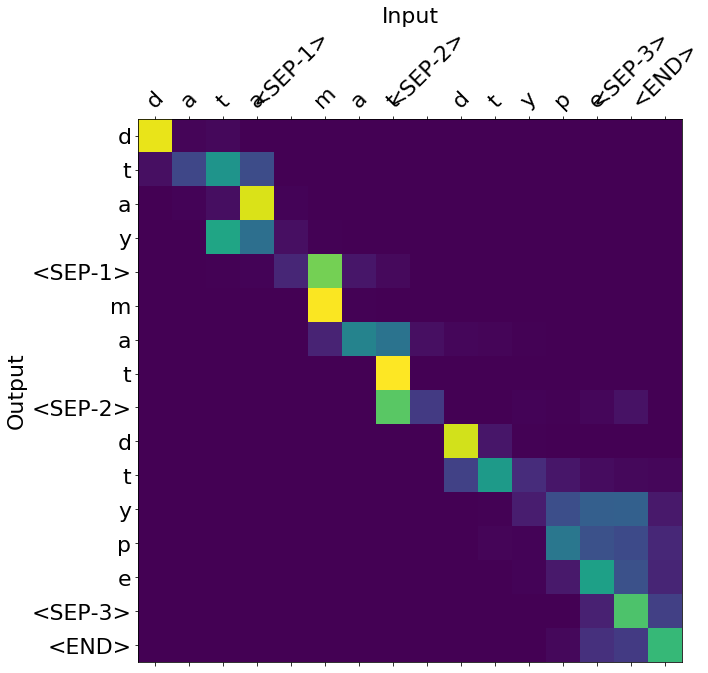
\includegraphics[width=0.8\linewidth]{images/typical_attention.png}
\end{figure}

\begin{table}
\begin{center}
\begin{tabular}{ | c || c |}
    \hline
    \hline
    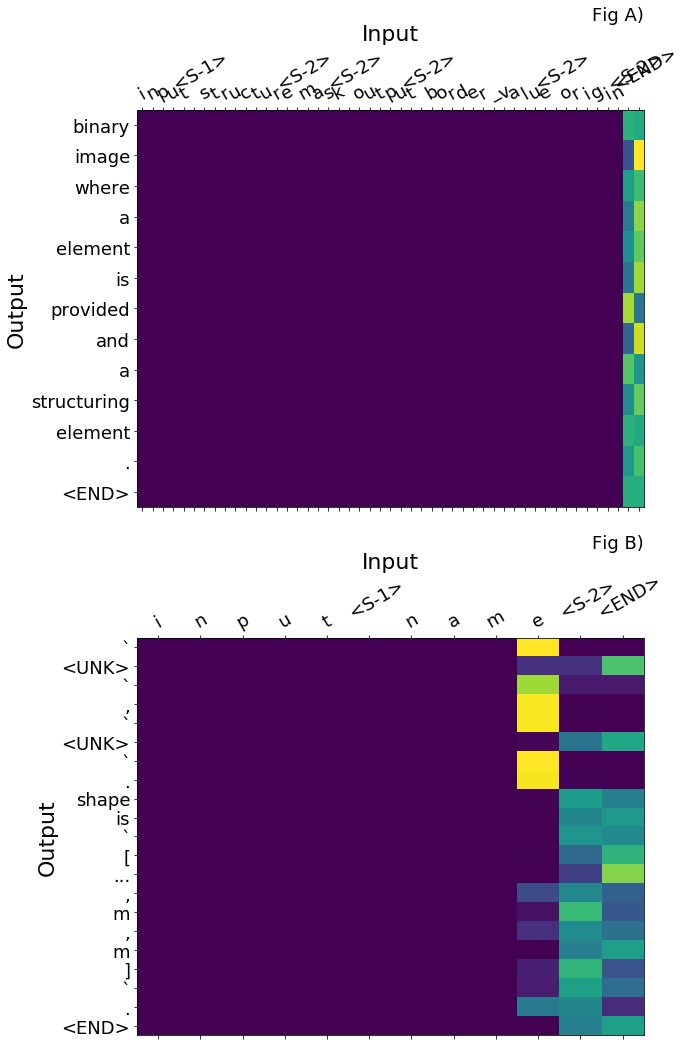
\includegraphics[width=0.5\linewidth]{images/otherargs_example.png}
    &
    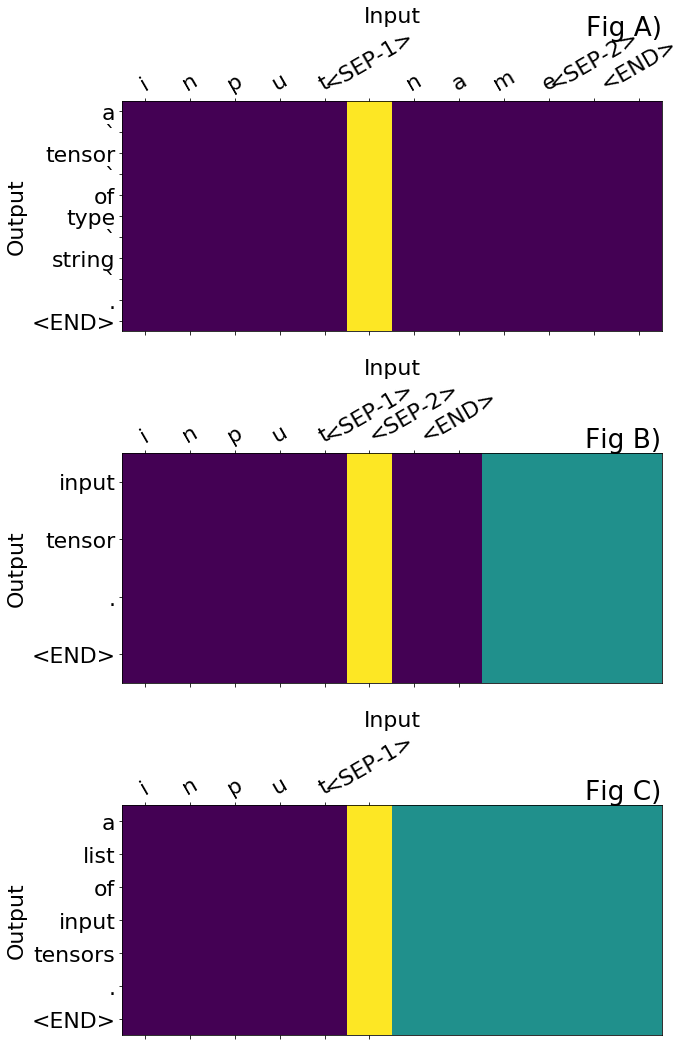
\includegraphics[width=0.5\linewidth]{images/different_translations_dupsXotherargs_3230minib.png} \\


    \hline

    \hline
\end{tabular}
\end{center}
\end{table}



\begin{table}
\begin{center}
\begin{tabular}{ l  }

\textbf{Nonsense}\\

\textbf{I}: \mintinline[]{python}{i n p u t <SEP-1> s t r u c t u r e <SEP-2> m a s k <SEP-2> o u t p}...\\
...\mintinline[]{python}{u t <SEP-2> b o r d e r _ v a l u e <SEP-2> o r i g i n <SEP-2> <END>}\\
\textbf{D}: binary image to be propagated inside ` mask ` .\\
\textbf{P}: binary image where a element is provided and a structuring element . $<$END$>$\\
\\\hline\\


\textbf{Overfitting}\\

\textbf{I}: \mintinline[]{python}{e n c o d i n g _ t y p e <SEP-1> s e l f <SEP-2> d o c u m e}...\\
...\mintinline[]{python}{n t <SEP-2> r e t r y <SEP-2> t i m e o u t <SEP-2> <END>}\\
\textbf{D}: the encoding type used by the api to calculate offsets .\\
\textbf{P}: the encoding type used by the api to calculate sentence offsets . \\
\\\hline\\




\textbf{Underdetermination}\\

\textbf{I}: \mintinline[]{python}{i n p u t <SEP-1> n a m e <SEP-2> <END>}\\
\textbf{D}: a ` tensor ` of type ` complex64 ` . a complex64 tensor .\\
\textbf{P}: ` $<$UNK$>$ ` , ` $<$UNK$>$ ` . shape is ` [ ... , m , m ] ` . \\
\\\hline\\

\\

\end{tabular}

\caption{Three examples of typical errors in the character Seq-to-Seq model.  In this case, the first example shows good use of data in the sequence but is nonsensical. The second is an example of overfitting where the predicted sentence is found in the dataset. The final case, multiple sequences such as these are found in the dataset, each with a different discription. Without looking at code, or function name (in this case) it is impossible to disambiguate and the model fails to make sense }
\end{center}
\end{table}

\begin{table}
\begin{center}
\begin{tabular}{l}

\hline
\textbf{Validation Example}\\

\textbf{I}: \mintinline[]{python}{i n p u t <SEP-1> s t r u c t u r e <SEP-2> m a s k <SEP-2> o u t p}...\\
...\mintinline[]{python}{u t <SEP-2> b o r d e r _ v a l u e <SEP-2> o r i g i n <SEP-2> <END>}\\
\textbf{D}: binary image to be propagated inside ` mask ` .\\
\textbf{P}: binary image where a element is provided and a structuring element . $<$END$>$\\
\\\hline\\

\textbf{Training Examples} starting \mintinline[]{yaml}{i n p u t <SEP-1> s t r u c t u r e}\\
\textbf{I}: \mintinline[]{yaml}{i n p u t <SEP-1> s t r u c t u r e 1 <SEP-2> s t r u c t u r}...\\
...\mintinline[]{yaml}{e 2 <SEP-2> o u t p u t <SEP-2> o r i g i n 1 <SEP-2> o r i g i n 2 <SEP-2> <END>}\\
\textbf{D}: binary image where a pattern is to be detected .\\
\\
\textbf{I}: \mintinline[]{yaml}{i n p u t <SEP-1> s t r u c t u r e <SEP-2> i t e r a t i o n s <SEP-2> o u t }...\\
...\mintinline[]{yaml}{p u t <SEP-2> o r i g i n <SEP-2> m a s k <SEP-2> b o r d e r _ v a l u e }\\
...\mintinline[]{yaml}{<SEP-2> b r u t e _ f o r c e <SEP-2> <END>}\\
\textbf{D}: binary array\_like to be closed . non-zero ( true ) elements form the subset to be closed .\\
\\
\textbf{I}: \mintinline[]{yaml}{i n p u t <SEP-1> s t r u c t u r e <SEP-2> o u t p u t <SEP-2> o r}...\\
...\mintinline[]{yaml}{i g i n <SEP-2> <END>}\\
\textbf{D}: n-dimensional binary array with holes to be filled\\
\\
\textbf{I}: \mintinline[]{yaml}{i n p u t <SEP-1> s t r u c t u r e <SEP-2> o u t p u t <SEP-2> <END>}\\
\textbf{D}: an array-like object to be labeled . any non-zero values in ` input ` are counted as features...\\
...and zero values are considered the background .\\
\\
\textbf{I}: \mintinline[]{yaml}{i n p u t <SEP-1> s t r u c t u r e <SEP-2> i t e r a t i o n s <SEP-2> m a s k }...\\
...\mintinline[]{yaml}{<SEP-2> o u t p u t <SEP-2> b o r d e r _ v a l u e <SEP-2> o r i g i n <SEP-2>}\\
...\mintinline[]{yaml}{b r u t e _ f o r c e <SEP-2> <END>}\\
\textbf{D}: binary image to be eroded . non-zero ( true ) elements form the subset to be eroded .\\
\\
\textbf{I}: \mintinline[]{yaml}{i n p u t <SEP-1> s t r u c t u r e <SEP-2> i t e r a t i o n s <SEP-2> m a s k}...\\
...\mintinline[]{yaml}{<SEP-2> o u t p u t <SEP-2> b o r d e r _ v a l u e <SEP-2> o r i g i n <SEP-2>}\\
...\mintinline[]{yaml}{b r u t e _ f o r c e <SEP-2> <END>}\\
\textbf{D}: binary array\_like to be dilated . non-zero ( true ) elements form the subset to be dilated .\\
\\



\end{tabular}

\caption{A validation example and the a selection of training points. Despite being a long sequence, }
\end{center}
\end{table}

\begin{enumerate}
    \item The rnn final state acts as a good contextual vector for generation, we get good performance improvements on decoding
    \item However, the attention is being pathological. It's such a good trategy, that it stays there, and stops looking elsewhere, the weight decays to zero
    \item then when you get to genuinely hard points - where attention is useful, it cant learn and it panics (see bluring at end - can only explore nearest by states)/
    \item this pattern is noticeable in other locations, moving the lstm to more data (with duplicates), we learn that the lstm learns
\end{enumerate}


\begingroup
\begin{table}
\begin{center}
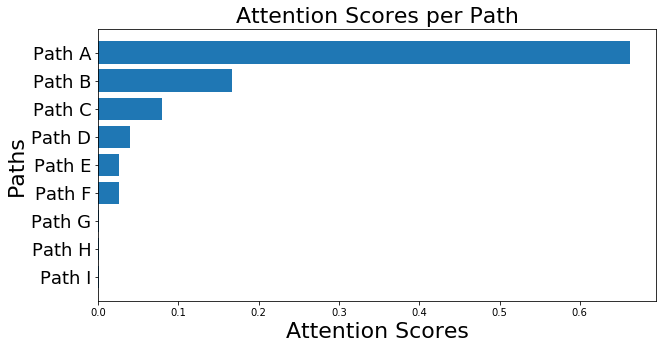
\includegraphics[width=0.8\linewidth]{ImagesCodeRelated/attention_xkcd.png}
    \fontsize{10pt}{12pt}\selectfont
        % how to set font size here to 10 px ?  
\begin{tabular}{c l}
    & \textbf{Paths} \\
    \\
    \textbf{Path A} & Name $\leftarrow$ comprehension $\leftarrow$ ListComp $\leftarrow$ Assign $\rightarrow$ Name : \mintinline[]{yaml}{palette} \\
    \textbf{Path B} & Name $\leftarrow$ comprehension $\leftarrow$ ListComp $\leftarrow$ Assign $\leftarrow$ FunctionDef[...] \\
        & [...]$\rightarrow$ Assign $\rightarrow$ ListComp $\rightarrow$ comprehension : \mintinline[]{yaml}{<UNK>} \\
    \textbf{Path C} & $<$UNK$>$ : \mintinline[]{yaml}{color_palette} \\
    \textbf{Path D} & Name $\leftarrow$ comprehension $\rightarrow$ Name : \mintinline[]{yaml}{name} \\
    \textbf{Path E} & $<$UNK$>$ : \mintinline[]{yaml}{palette} \\
    \textbf{Path F} & $<$UNK$>$ : \mintinline[]{yaml}{palette} \\
    \textbf{Path G} & $<$UNK$>$ : \mintinline[]{yaml}{len} \\
    \textbf{Path H} & $<$UNK$>$ : \mintinline[]{yaml}{name} \\
    \textbf{Path I} & $<$UNK$>$ : \mintinline[]{yaml}{<UNK>} \\
\end{tabular}
\end{center}

\caption{Example Attention Scores}
\end{table}
\endgroup

\begin{listing}[h!] 
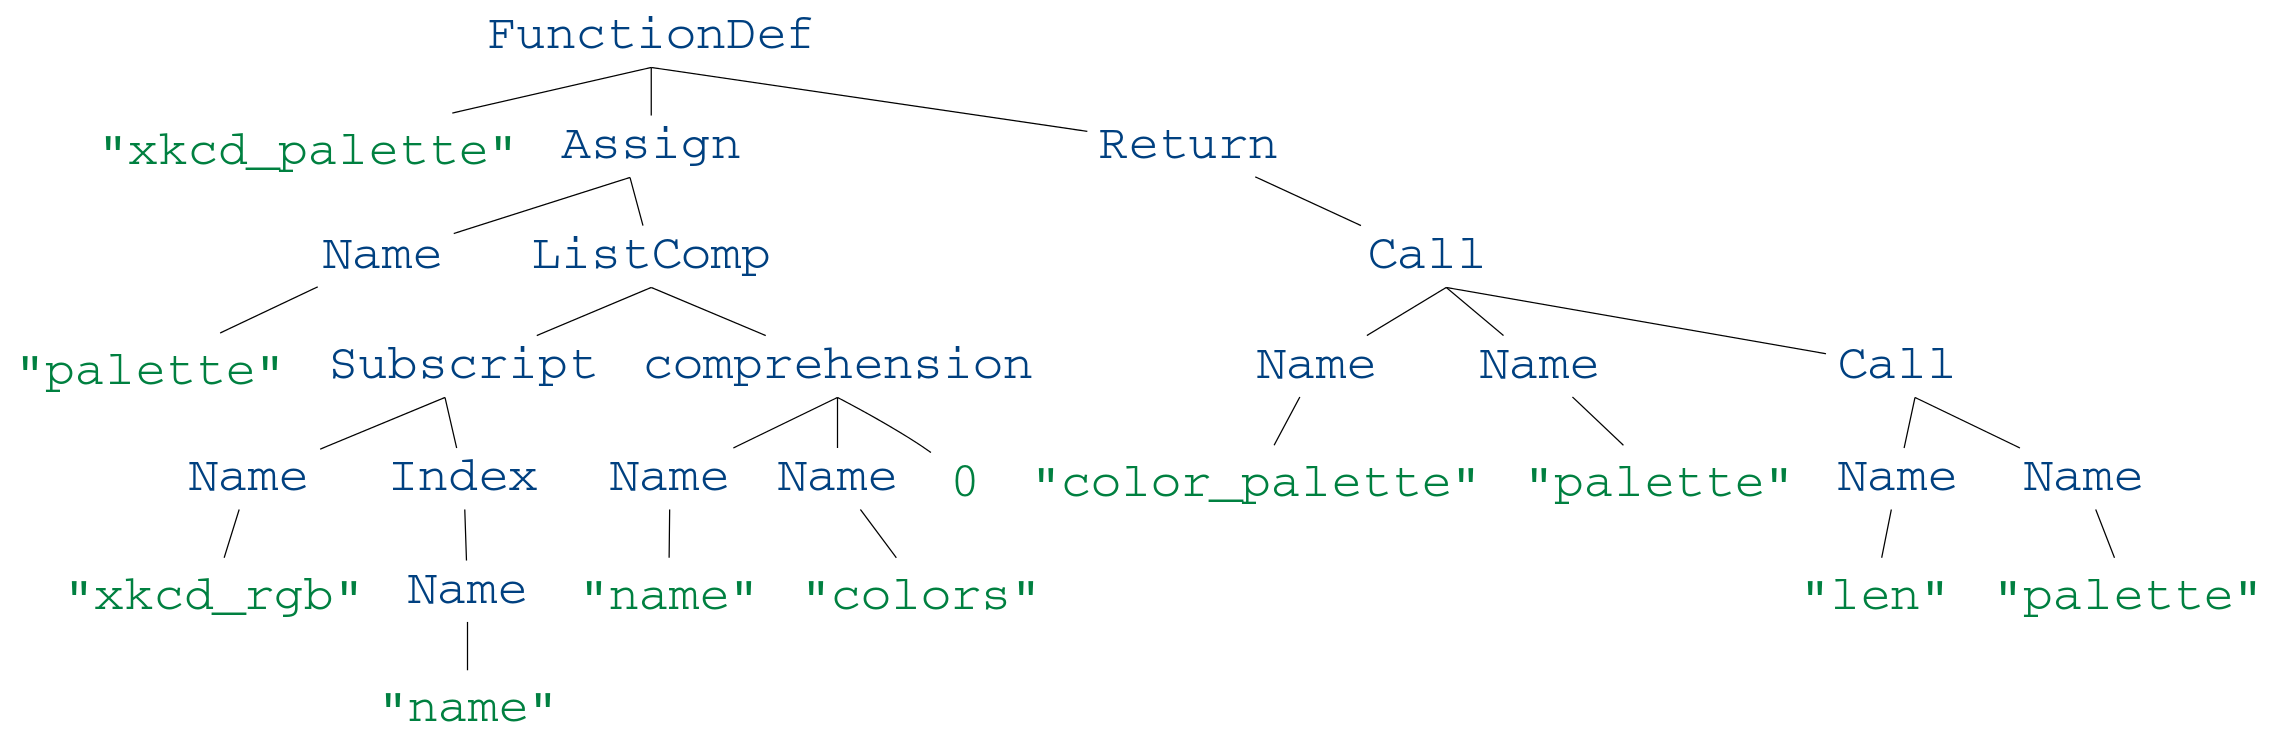
\includegraphics[width=0.8\linewidth]{ImagesCodeRelated/xkcd_palette_strip.png}
\begin{minted}[]{python}
def xkcd_palette(colors):
    palette = [xkcd_rgb[name] for name in colors]
    return color_palette(palette, len(palette))

\end{minted}
\begin{tabular}{l}
\textbf{I}: \mintinline[]{python}{colors}\\
\textbf{D}: list of keys in the `` seaborn.xkcd\_rgb `` dictionary .\\
\textbf{P}: a list of data to read . if none , all other the first will be returned .\\
\end{tabular}

\caption{Code \& List}
\end{listing}

\begin{figure}
\begin{center}
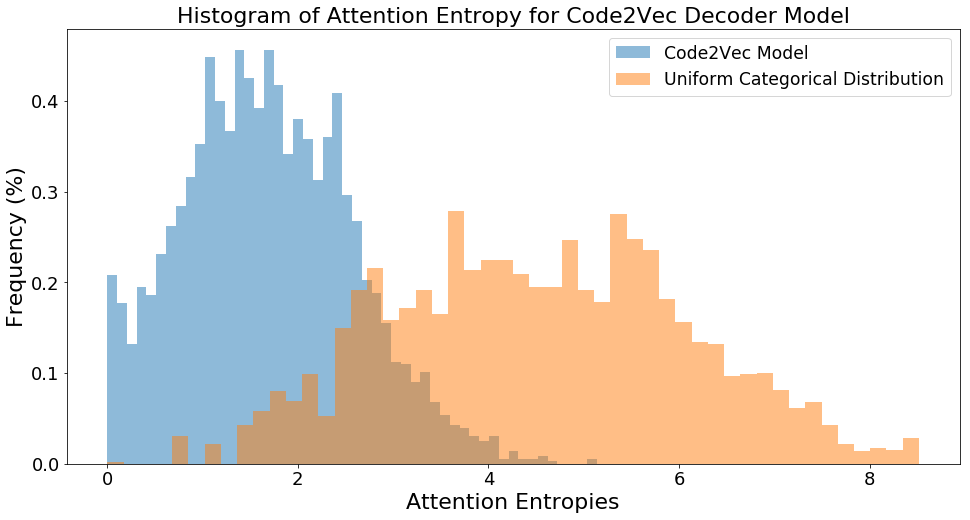
\includegraphics[width=.8\linewidth]{ImagesCodeRelated/code2vec_entropies.png}
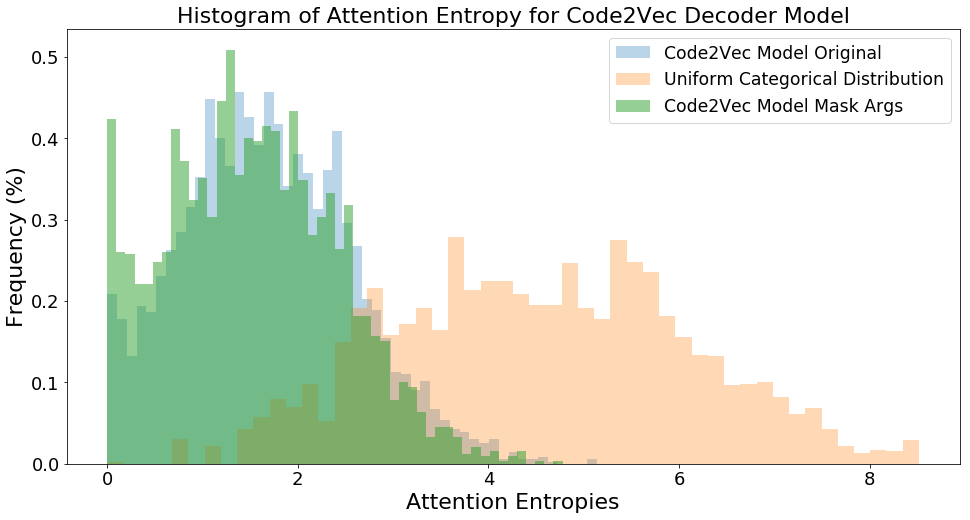
\includegraphics[width=0.6\linewidth]{ImagesCodeRelated/entropies_mask_args.png} 
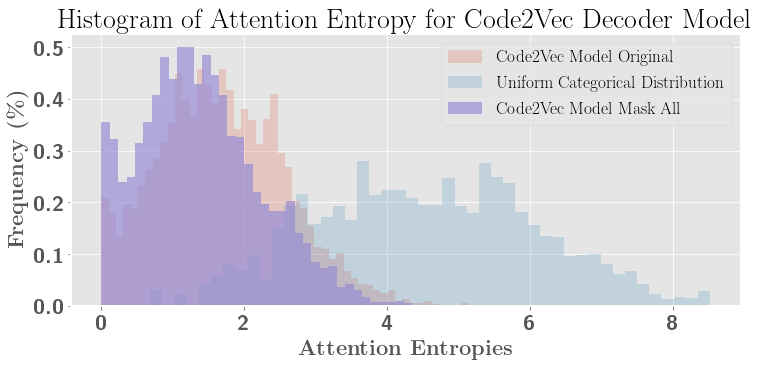
\includegraphics[width=0.6\linewidth]{ImagesCodeRelated/entropies_mask_all.png}
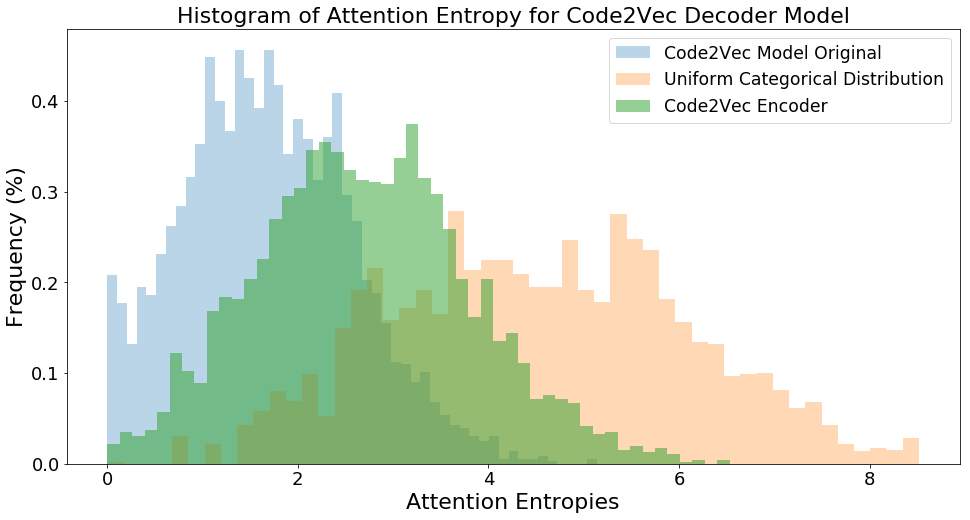
\includegraphics[width=.8\linewidth]{ImagesCodeRelated/save_c2e_encoder.png}
\end{center}
\end{figure}

% 
\chapter{Another Appendix About Things}
\label{appendixlabel2}
(things)

\chapter{Colophon}
\label{appendixlabel3}
\textit{This is a description of the tools you used to make your thesis. It helps people make future documents, reminds you, and looks good.}

\textit{(example)} This document was set in the Times Roman typeface using \LaTeX\ and Bib\TeX , composed with a text editor. 
 % description of document, e.g. type faces, TeX used, TeXmaker, packages and things used for figures. Like a computational details section.
% e.g. http://tex.stackexchange.com/questions/63468/what-is-best-way-to-mention-that-a-document-has-been-typeset-with-tex#63503

% Side note:
%http://tex.stackexchange.com/questions/1319/showcase-of-beautiful-typography-done-in-tex-friends 
  
% This line manually adds the Bibliography to the table of contents.
% The fact that \include is the last thing before this ensures that it
% is on a clear page, and adding it like this means that it doesn't
% get a chapter or appendix number.
\addcontentsline{toc}{chapter}{Bibliography}

% Actually generates your bibliography.
\bibliography{betterbib}


% \appendix


% \begin{thebibliography}{HHM99}


% \bibitem[Pri70]{PriorNOP70}  %%only an example
% A.~Prior.
% \newblock The notion of the present.
% \newblock {\em Studium Generale}, 23:  245--248, 1970.


% \bibitem[Rey97]{Rey:D}
% M.~Reynolds.
% \newblock A decidable temporal logic of parallelism.
% \newblock {\em Notre Dame Journal of Formal Logic}, 38(3):  419--436,
%   1997.
% \end{thebibliography}
% \chapter{Other appendices, e.g. code listing}

\end{document}